%%%%%%%%%%%%%%%%%%%%%%%%%%%%%%%%%%%%%%%%%%%%%%%%%%%%%%%%%%%%%%%
\section{Photon Detection System Design}
\label{sec:fdsp-pd-design}
%\metainfo{(Length: \dword{tdr}=50 pages, TP=20 pages)}
%\metainfo{\color{blue} Content: Warner, WG Conveners}

% Everything in this section is about the 10kt module now
%\subsubsection{ARAPUCA Configuration in DUNE \SI{10}{kt} }
%\label{sssec:arapuca-dune}

%\fixme{Update with x-arapuca as baseline configuration.}

The principal task of the \dword{spmod} \dword{pds} is to measure the \dword{vuv} scintillation light produced by ionizing tracks in the TPC within the geometrical constraints of the \dword{apa} structure. 
The modular arrangement of the \dword{spmod} TPC calls for a configuration across the width of the cryostat starting with an \dword{apa} plane against one cryostat wall, and following with \dwords{apa} and \dwords{cpa} arranges as follows:  APA-CPA-APA-CPA-APA. This means that the central \dword{apa} will collect charge and see scintillation light from \lar volumes on both sides, whereas those by the wall collect from only one side. 

%A commercially available compact solution for photon measurement is the \dword{sipm}, however, the response of the devices, which typically peaks in the visible range (>\SI{400}{nm}) is not well-matched to incident \SI{127}{nm} scintillation photons, so a wavelength shifter or some sort must be employed.  In addition, even though production cost and key performance parameters have improved significantly in recent years, the cost of the readout electronics (channel count) and the \dword{sipm}s needed to meet the physics requirements of the \dword{pds} would be prohibitive. 

The light collector design must optimize the costs of various components of the system while meeting the performance requirements.  It will use \dwords{sipm}, which provide a commercially available compact solution for photon measurement.  However, the response of these devices, which typically peaks in the visible range (>\SI{400}{nm}), is not well-matched to incident \SI{127}{nm} scintillation photons, so a wavelength shifter or some sort is required.  In addition, even though production cost and key performance parameters have improved significantly in recent years, covering the light detector surfaces with enough \dwords{sipm} to meet the physics requirements of the \dword{pds} would be cost-prohibitive. 

% In practice, this consists of collecting \dword{vuv} photons produced throughout a volume of thousands of cubic-meters (viewing the entire \SI{10}{kt} \lar fiducial mass), converting the photons to longer wavelengths and guiding them onto \dwords{sipm} that are typically less than \SI{1}{cm$^2$} in area. 
%For reference, an array of \num{48} \dwords{sipm} demonstrated a detection efficiency of \SI{13}{\%}, corresponding to an effective area of \SI{2.2}{cm$^2$}. This array, tested in the \fnal \dword{tallbo} \lar facility, consisted of twelve \num{4}$\times$\num{4} units of \SI{3}{mm}$\times$\SI{3}{mm} sensL C-series coated with \SI{100}{$\mu$g/cm$^2$} of \dword{tpb}. 

%A challenge for the \dword{pds} is that a full set of requirements is not yet fully defined for one of the priority physics topics, \dword{snb} neutrinos. So the designs strive to demonstrate that at minimum the requirements for the accelerator neutrino program, atmospheric neutrinos and nucleon decay will be met, while maintaining the flexibility to adjust to the greater demands for the SBN physics.


The \dword{pds} baseline design %presented in this section 
implements a light trapping concept called ARAPUCA that reduces the number of required \dwords{sipm}. This and two other light collector options were investigated in detail over several years, the others %two 
based on %the concept of 
wavelength-shifter coated light guides. 
The baseline ARAPUCA-based design,  meets or exceeds the DUNE requirements presented in Section~\ref{sec:fdsp-pd-intro}. In addition, the design has the flexibility to accommodate greater demands, such as might be desired for SBN physics, without major changes to the design and which could be adopted quite late in the final design stages.
The ARAPUCA concept uses dichroic filter windows to form an effective light trap that increases the efficiency for light collection onto the \dwords{sipm}. %silicon photomultiplier photosensors. 
%A design using this has been adopted for the baseline design. 
 The DUNE Single-Phase Photon Detector Design Report~\citedocdb{11644} provides many additional details on the design too specialized for the scope of this TDR.  
 
While the ARAPUCA modules deployed in \dword{pdsp} collect light from only one direction, an advanced design called X-ARAPUCA can be deployed as either single-face or dual-face readout by using either an opaque reflector plate (single) or a second dichroic filter window (dual) on the second face. 
Figure~\ref{fig:3dtpc-pd} shows how a light-collector module is incorporated into an \dword{apa}. An identical modular mounting scheme was used for each of the options investigated. One module spans the width of an \dword{apa}.

%\fixme{It would be good to have a figure here - Dave can you make one like fig. 1.2 that has x-arapucas?}
\fixme{Dave W:  I will make a new version of this figure showing X-ARAPUCAs in time for the second draft.}

%This section summarizes all aspects of the design and implementation of \dword{pds} in the \spmod. %10kt far detector single phase detector system.  
%Many additional details too specialized for the scope of this TDR are to be found in the DUNE Single-Phase Photon Detector Design Report, which (is in the process of being developed and) can be found in \citedocdb{11644}.
%\fixme{docDB reference needed--  Bob, not sure how to make a reference to this..}

%In the following we summarize the design and development status for each light collector option\footnote{For the \dword{tdr} there will be a baseline design and at most one alternative.}.

%At the time of the \dword{tp} there are three light collector options under consideration; Figure~\ref{fig:3dtpc-pd} shows how they are incorporated into the TPC anode plane assembly by an identical modular mounting scheme. In the following we summarize the design and development status for each light collector option\footnote{For the \dword{tdr} there will be a baseline design and at most one alternative.}.

%%%%%%%%%%%%%%%%%%%%%%%%%%%%%%%%%%%
\subsection{Light Collector}
\label{ssec:fdsp-pd-pc-arapuca}

The %\dword{pds} light collector uses the 
ARAPUCA concept %described in Section~\ref{sssec:photoncollectors}, which 
takes advantage of a new approach to \lar scintillation photon detection where the effective photon detection area is increased by trapping photons inside a box (cell) with highly reflective internal surfaces until reflections guide them to active photosensors of relatively small area. % \dword{sipm}~\cite{arapuca_jinst}. 

Photon trapping is achieved through a novel use of wavelength-shifting and the technology of the dichroic shortpass optical filter. These commercially available filters are created by using multilayer thin films that %have the property of being 
are highly transparent 
to photons with a wavelength below a tunable cutoff, %while being 
with transmission typically greater than 95\%, yet almost perfectly reflective to photons with a wavelength above the cutoff.  Such a filter coated with either one or two different wavelength-shifters, depending on the detailed implementation, forms the entrance window to a flat cell whose %other 
internal surfaces are covered by highly reflective acrylic foils
%(3M-Vikuiti ESR \footnote{3M Vikuiti\texttrademark\ ~foils. https://en.wikipedia.org/wiki/Vikuiti.}, for example), 
except for a small fraction %of the surface that is 
occupied by \dwords{sipm}.

%To act as a photon trap, the wavelength-shifter deposited on the outer face of the dichroic filter must have its emission wavelength less than the cut-off wavelength of the filter, below which transmission is typically greater than 95\%. 
For the collector to act as a photon trap, the emission wavelength of the wavelength-shifter deposited on the outer face of the dichroic filter must be less than the cutoff wavelength of the filter. 
%, below which transmission is typically greater than 95\%. 
The transmitted photons pass through the filter where they encounter a second wavelength shifter %either on the inner surface of the filter or coated on the reflecting inner surfaces of the box, 
with an emission spectrum greater than the cutoff wavelength, thus trapping them. The location of the second wavelength shifter is different in the single- and dual-face cells. \fixme{In a single-face cell, the filter is coated also on the inside surface with a wavelength shifter; in a dual-face cell check and come back}

Trapped photons reflect off the inner walls and the filter surface(s) (of reflectivity typically greater than \SI{98}{\%}) 
and have a high probability %to be incident 
of impinging on a \dword{sipm} before being lost to absorption. The concept is illustrated in Figure~\ref{fig:arapuca}. 
 A proof-of-principle validation of the ARAPUCA concept is described in Section~\ref{sec:proof-principle}.
%It is easy to show that, for small values of \dword{sipm} coverage of the internal surface, the amplification factor is equal to $A=1/(2(1-R))$, where R is the average value of the reflectivity of the internal surfaces; for an average reflectivity of 0.95 the amplification factor is equal to ten.

\begin{dunefigure}[Schematic representation of the ARAPUCA operating principle.]{fig:arapuca}
{Schematic representation of the ARAPUCA operating principle. This example assumes a filter cutoff of \SI{400}{nm}.}
%  %\includegraphics[height=5cm]{pds-arpkscheme}   
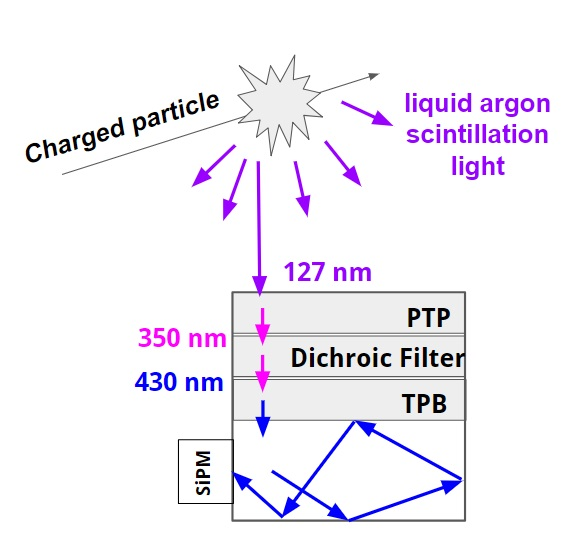
\includegraphics[height=5cm]{pds-arapuca-concept}   
\end{dunefigure}

%\subsubsection{X-ARAPUCA} 
%\label{sssec:x-arapuca}
The X-ARAPUCA, adopted for the baseline design, is an evolution of the ARAPUCA concept that further improves the collection efficiency, while retaining the same working principle, mechanical form factor and active photosensitive coverage. It adds a 
short acrylic wavelength-shifting light guide (Eljen EJ-296) inside the cell in which trapped photons are converted and transported to the readout via total internal reflection. 
X-ARAPUCA, Figure~\ref{fig:pds-x-arapuca-cell},  is thus effectively a hybrid solution between the ARAPUCA and the wavelength-shifting light guide concepts. 

A fraction of the photons are converted inside the light guide and guided to the readout. Other photons,  e.g,. those at small angle of incidence below the critical angle of the light guide, % slab, 
 after conversion at %the slab 
 its surface %will 
 remain trapped in the cell and are eventually collected by the \dwords{sipm}, as in a standard ARAPUCA cell.
 
This solution minimizes the number of reflections on the internal surfaces of the cell and thus the probability of photon loss. Simulations suggest that this modification will lead to a significant increase of the collection efficiency, to around 60\%, so the photon detection efficiency including the \dword{sipm} response in principle could approach 20\%. Results from prototype measurements are presented in Sections~\ref{sec:xarapuca-unicamp} and \ref{sec:iceberg-teststand}.

 \begin{dunefigure}[Simplified conceptual model depicting a single filter cell of an X-ARAPUCA design: assembled cell (left),  exploded view (right).]{fig:pds-x-arapuca-cell}
{Simplified conceptual model depicting a %single 
dual-face filter cell of an X-ARAPUCA design: assembled cell (left),  exploded view (right). The yellow plates represent the dicrhoic filters (coated on their outside surfaces with wavelength shifter), the blue plate represents the light guide, and the \dwords{sipm} are shown on the right side of the cell. The size and aspect ratio of the cells can be adjusted to match the spatial granularity required for a \dword{pd} module. The cell is shown laying on its side; it stands vertically when mounted in an \dword{apa}.} 
 % \vspace{-2.5cm}
 %two-sided x-arapuca 4/14/18 
  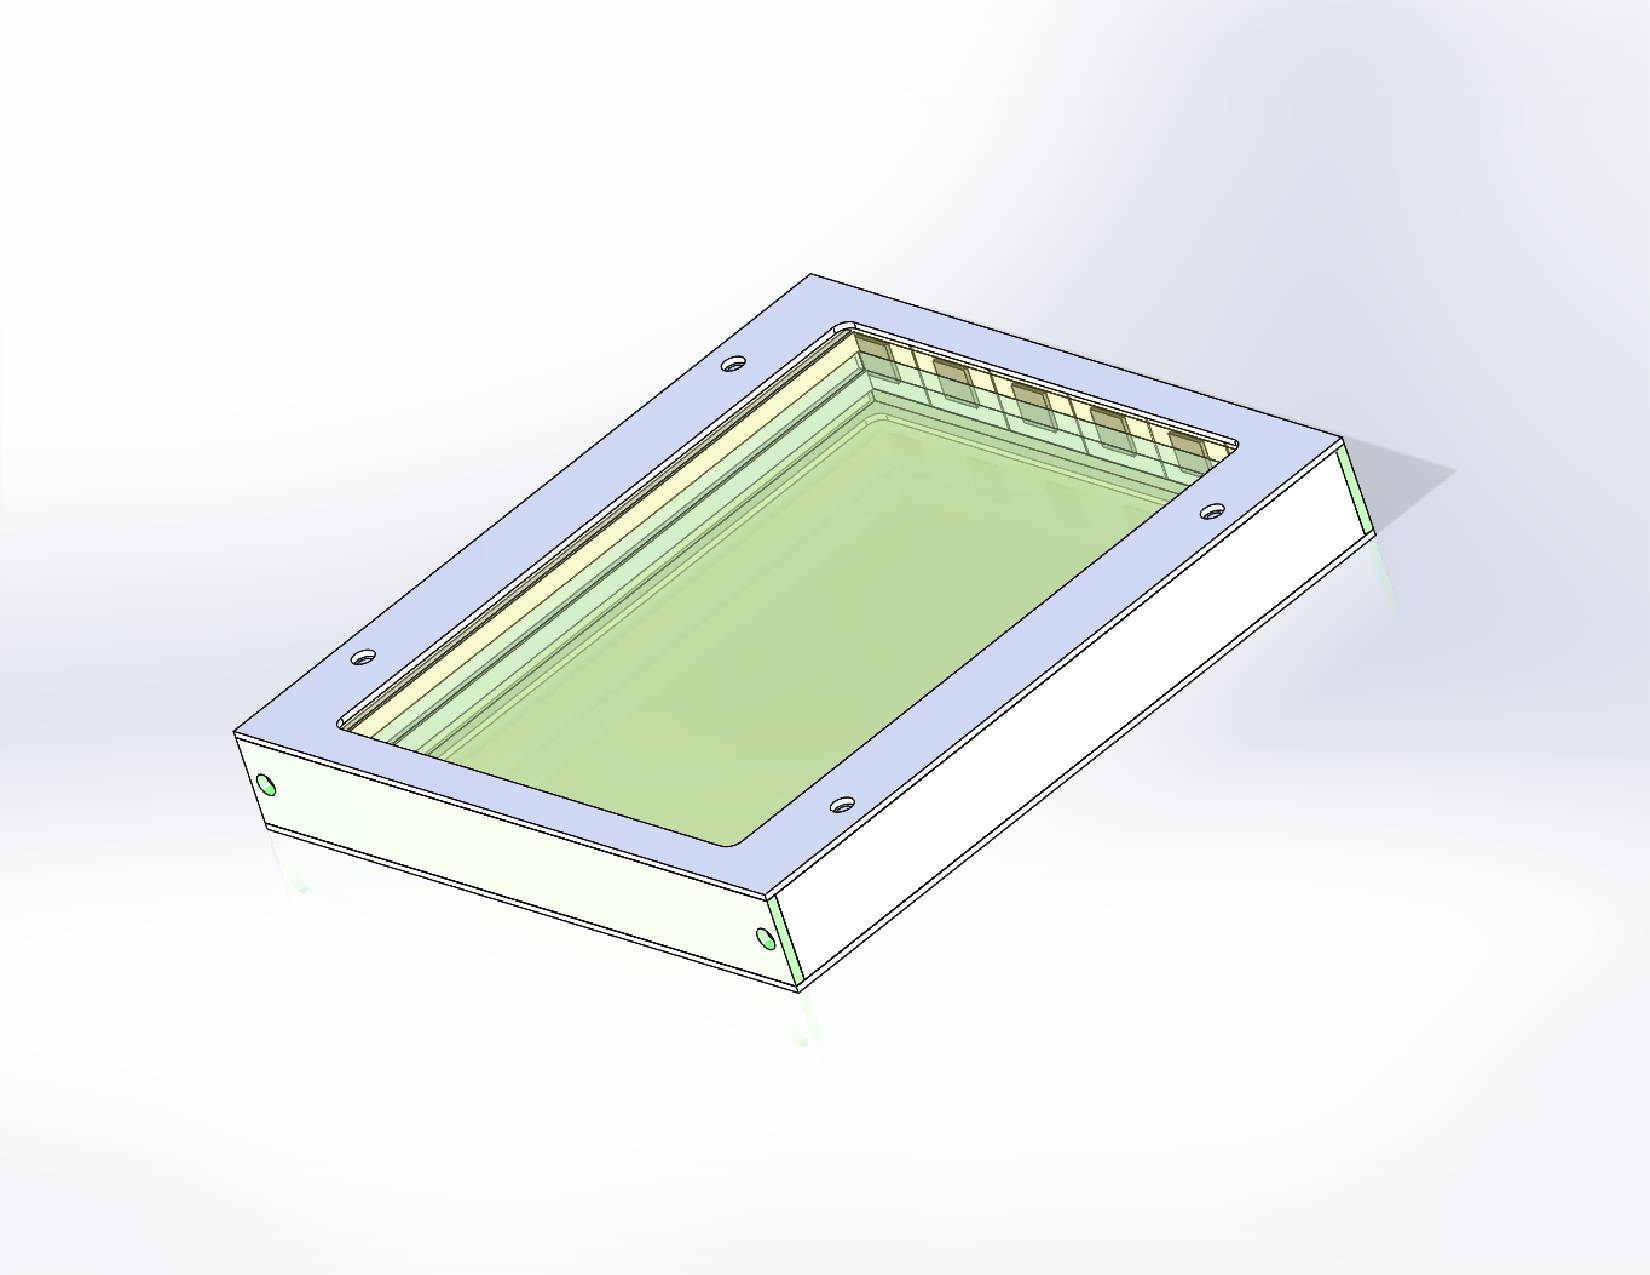
\includegraphics[height=.25\textheight]{pds-x-arapuca-cell}
  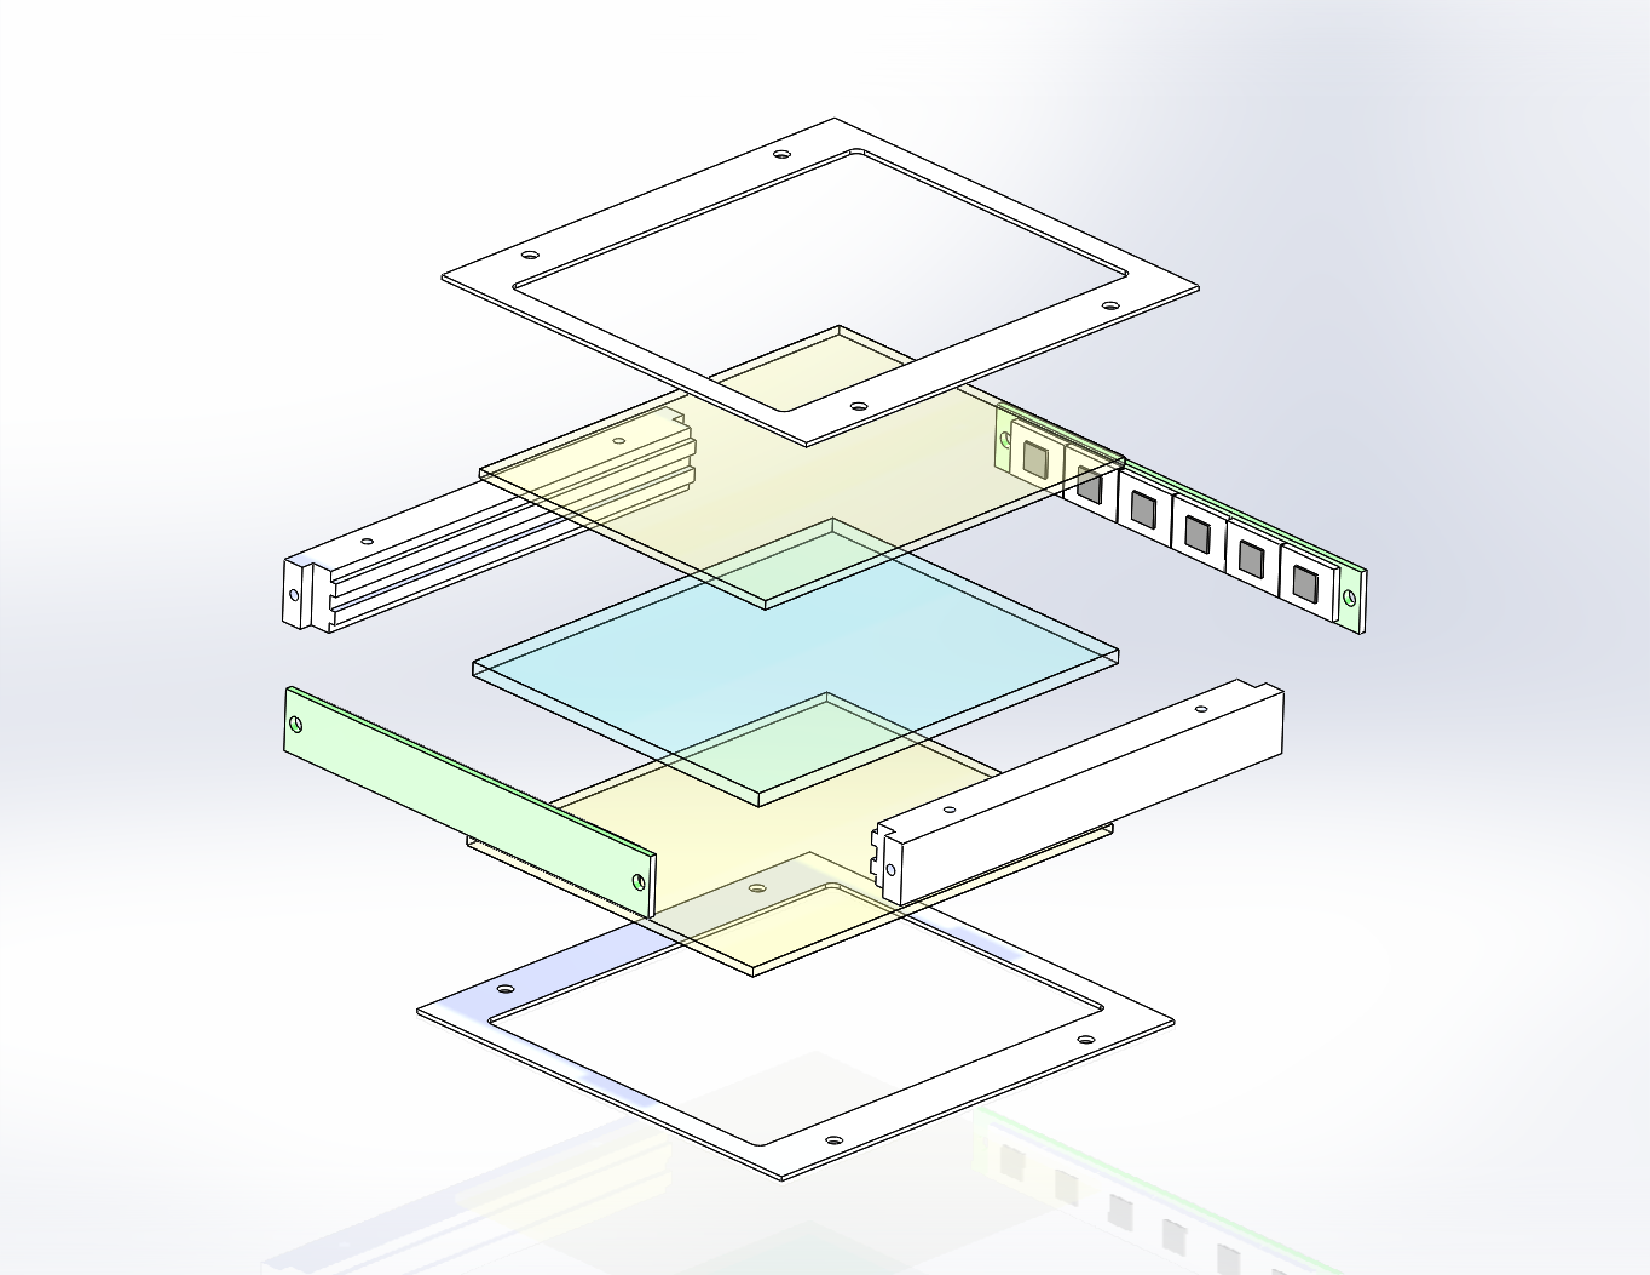
\includegraphics[height=.25\textheight]{pds-x-arapuca-exploded-view}
\end{dunefigure}

%\fixme{modifying descriptive text below}
%In the X-ARAPUCA design, Figure~\ref{fig:pds-x-arapuca-cell}, the inner shifter coating/lining over the reflective walls of the box is replaced by a thin wavelength-shifting light guide slab inside the box, of the same dimensions of the acceptance filter window and parallel to it. The \dword{sipm} arrays are installed vertically on the sides of the box, parallel to the light guide thin ends. 
%In the X-ARAPUCA design, Figure~\ref{fig:pds-x-arapuca-cell}, a single acrylic wavelength shifting light guide (Eljen EJ-296) 
The light guide inside the cell is positioned behind an array of six dichroic filters and parallel to them. 
 \fixme{Anne proposes to remove: This thin wavelength-shifting slab replaces the inner shifter coating over the reflective walls in the \dword{pdsp} S-ARAPUCA design. }
This design is easily configurable to %be sensitive to 
detect light from just one side, as required for the side \dwords{apa}, or from both sides for the central \dwords{apa}. 

For dual-sided X-ARAPUCA modules, dichroic filters are placed on both sides of the %WLS bar. 
cell facing the \lar volumes.  In the case of the single-sided device, the back side of the cell  %dichroic filter is replaced by 
has a layer of highly-reflective Vikuiti\texttrademark\ to act as %the rear
a  reflector.  In both cases, the \dword{sipm} arrays are installed vertically on the sides of the cell, parallel to and up against the light guide thin ends, but with part of the active detection area free to collect the fraction of photons reflected off the cell walls. \fixme{check -Anne added this}

\fixme{take it up from here next week.}

The basic mechanical design of the X-ARAPUCA-based \dword{pd} modules for the first \dword{spmod} is similar to that of the two prototypes produced for \dword{pdsp}. Modifications to the prototype design include:  mechanical changes to allow for single-sided or double-sided readout; increase in light collection area made possible by larger slots in the \dword{apa}; and modifications to the cabling and connector plan required to move the \dword{pd} cables out of the APA side tubes, while reducing the cable requirements to one cat-6 cable per \dword{pd} module.

\fixme{can we remove this sentence? Here we describe the design, fabrication and assembly envisaged based on that experience and these evolved design considerations. (anne)}

Each X-ARAPUCA module is shaped as a bar with external dimensions of \SI{209.2}{cm}$ \times$ \SI{11.8}{cm} $\times$ \SI{2.3}{cm}, which allows for it to be inserted between the wire planes through 10 slots in the \dword{apa}. 

%\fixme{figure of full PD module (with outside dimensions) here}

\begin{dunefigure}[A full X-ARAPUCA module overview]
{fig:pds-x-arapuca-full-module}
{A full X-ARAPUCA module overview. A module, the width of an \dword{apa}, includes four supercells, each including six X-ARAPUCA cells. }
 %two-sided x-arapuca 4/14/18
   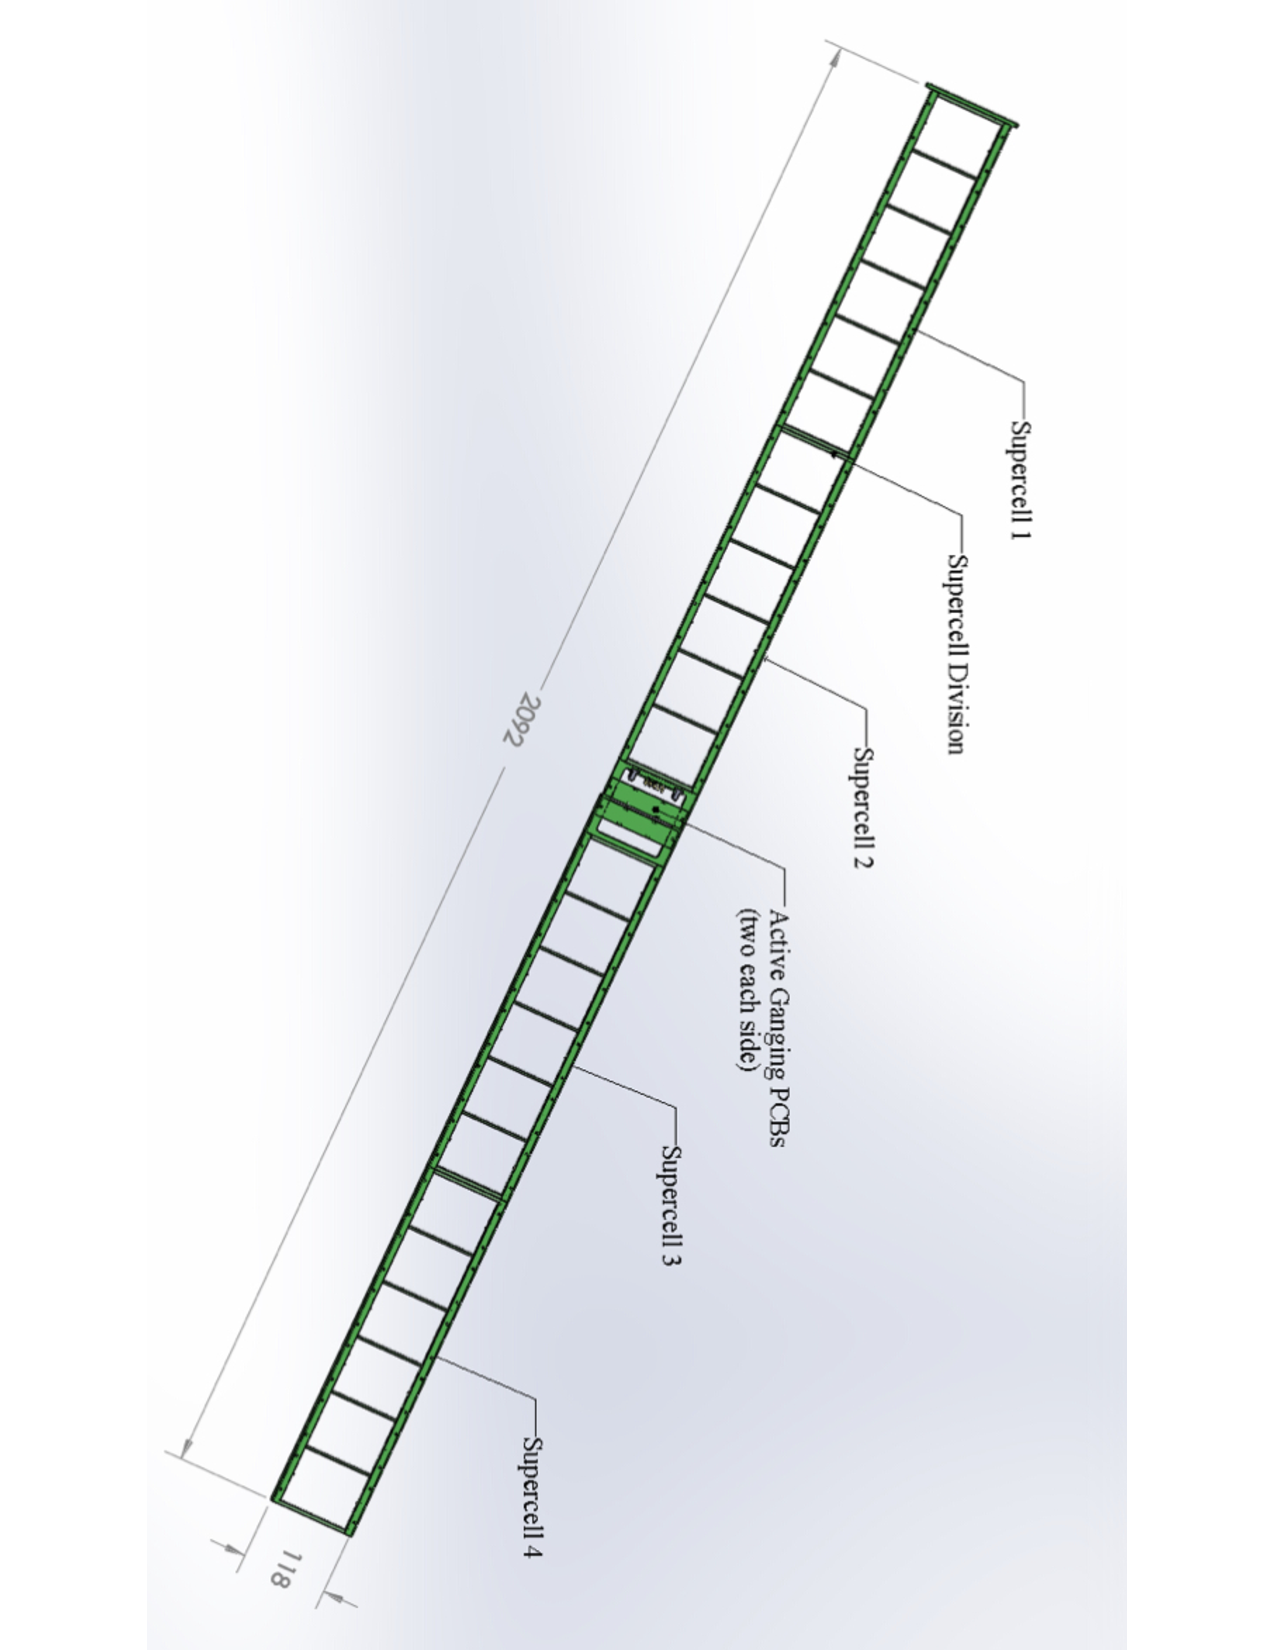
\includegraphics[angle=90,width=14cm]{pds-design-full-module-dimensioned}
  %\vspace{-2.5cm} 
\end{dunefigure}

The module contains four X-ARAPUCA supercells, each with six dichroic filter based optical windows (for the single-sided readout) or 12 windows(double-sided readout) with an area of \SI{7.8}{cm} $\times$ \SI{9.3}{cm}.  The internal dimensions of  a supercell are approximately \SI{48.8}{cm} $\times$ \SI{10.0}{cm} $\times$ \SI{0.8}{cm}. A WLS plate (Eljen EJ-286) of dimensions \SI{48.7}{cm} $\times$ \SI{93.0}{cm}$\times$ \SI{0.35}{cm} is centered in the supercell midway between the dichroic windows.  
 
%\fixme{insert exploded view of PD supercell, and dimensioned cross-section, here}

\begin{dunefigure}[Exploded X-ARAPUCA supercell.]{fig:pds-x-arapuca-exploded-Detail}
{Detailed exploded view of X-ARAPUCA supercell. Note that components are designed to be cut from FR-4 G-10 sheets to simplify fabrication.}
 % \vspace{-2.5cm}
 %two-sided x-arapuca 4/14/18
   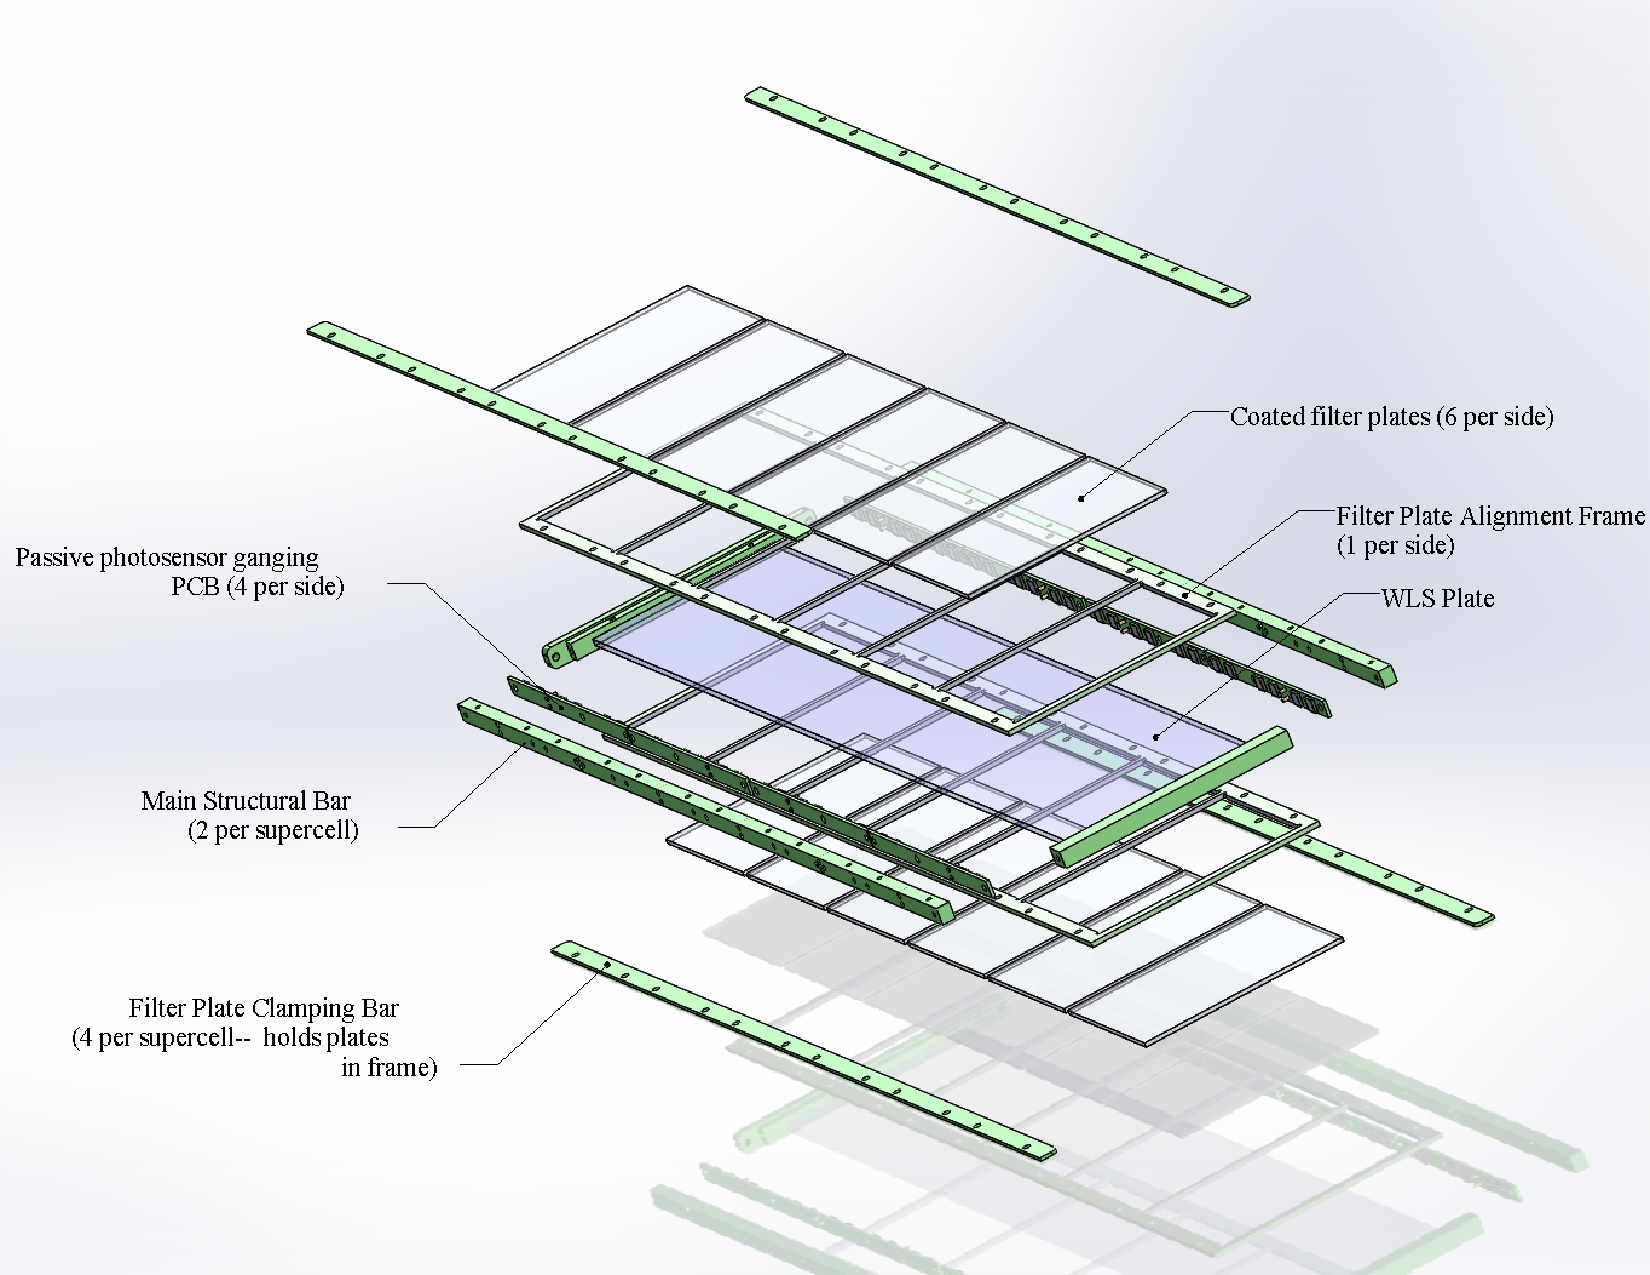
\includegraphics[height=.4\textheight]{pds-exploded-supercell-assembly-r2}
 % 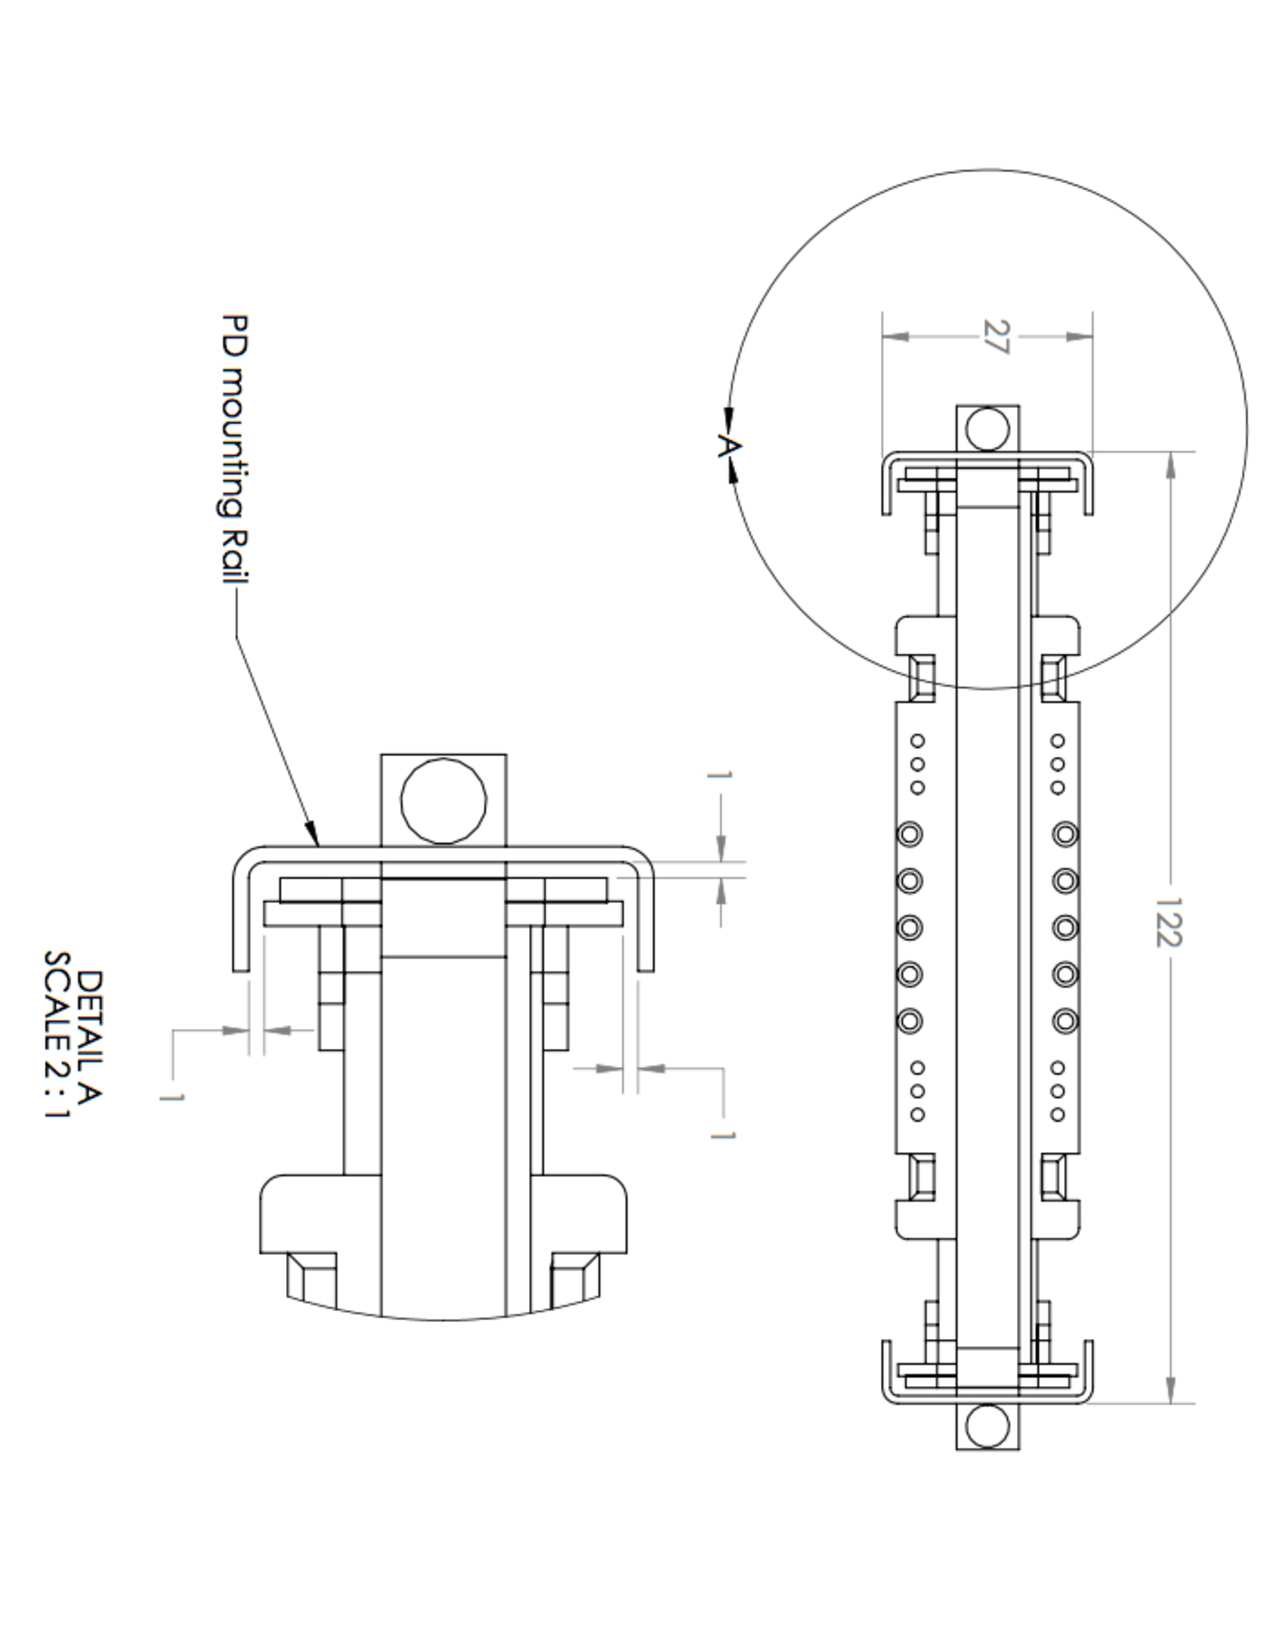
\includegraphics[height=.25\textheight]{pds_design_dimensioned_cross_section}
\end{dunefigure}

In order to reduce production costs and simplify fabrication, most of the PD components are designed to be water-jet cut from sheets of FR-4 G-10 material, with minimal post-cutting machining required (mostly the tapping of pre-cut holes).  The current design contains many small fasteners; we will investigate replacing some of the fasteners with epoxy lamination of cut sheets where appropriate and cost effective, as the design process matures.

The \dwords{sipm} are mounted to PCBs positioned on the long sides of the supercell.  The \dwords{sipm} are passively ganged in groups of six to photosensor mounting boards. Before mounting into the ARAPUCA module they are tested at room and LN2 temperatures. It is anticipated that the production of the boards for  \dwords{spmod} this will be done outside the USA and the design will be optimized by Latin American institutions. Eight \dword{sipm} mounting boards are used per supercell (for a total of 48 \dwords{sipm}).  The ganged signal outputs from these boards are connected to traces in signal routing boards at the edge of the module. These signal routing boards also act as mechanical elements in the design, mechanically joining the supercells and providing for rigidity.  These PCBs are 4-layer boards, approximately \SI{104.6}{cm} $\times$ \SI{2.3}{cm} $\times$ \SI{0.15}{cm}.

 \begin{dunefigure}[X-ARAPUCA SiPM mounting and signal routing boards.]
 {fig:mounting-board-routing-board}
{Model of photosensor mounting board (left) and signal routing PCB (right) for X-ARAPUCA module.  Six Hamamatsu \dwords{mppc} are passively ganged and the ganged signals transmitted along the routing board to the active ganging circuits in the center of the module}
 % \vspace{-2.5cm}
  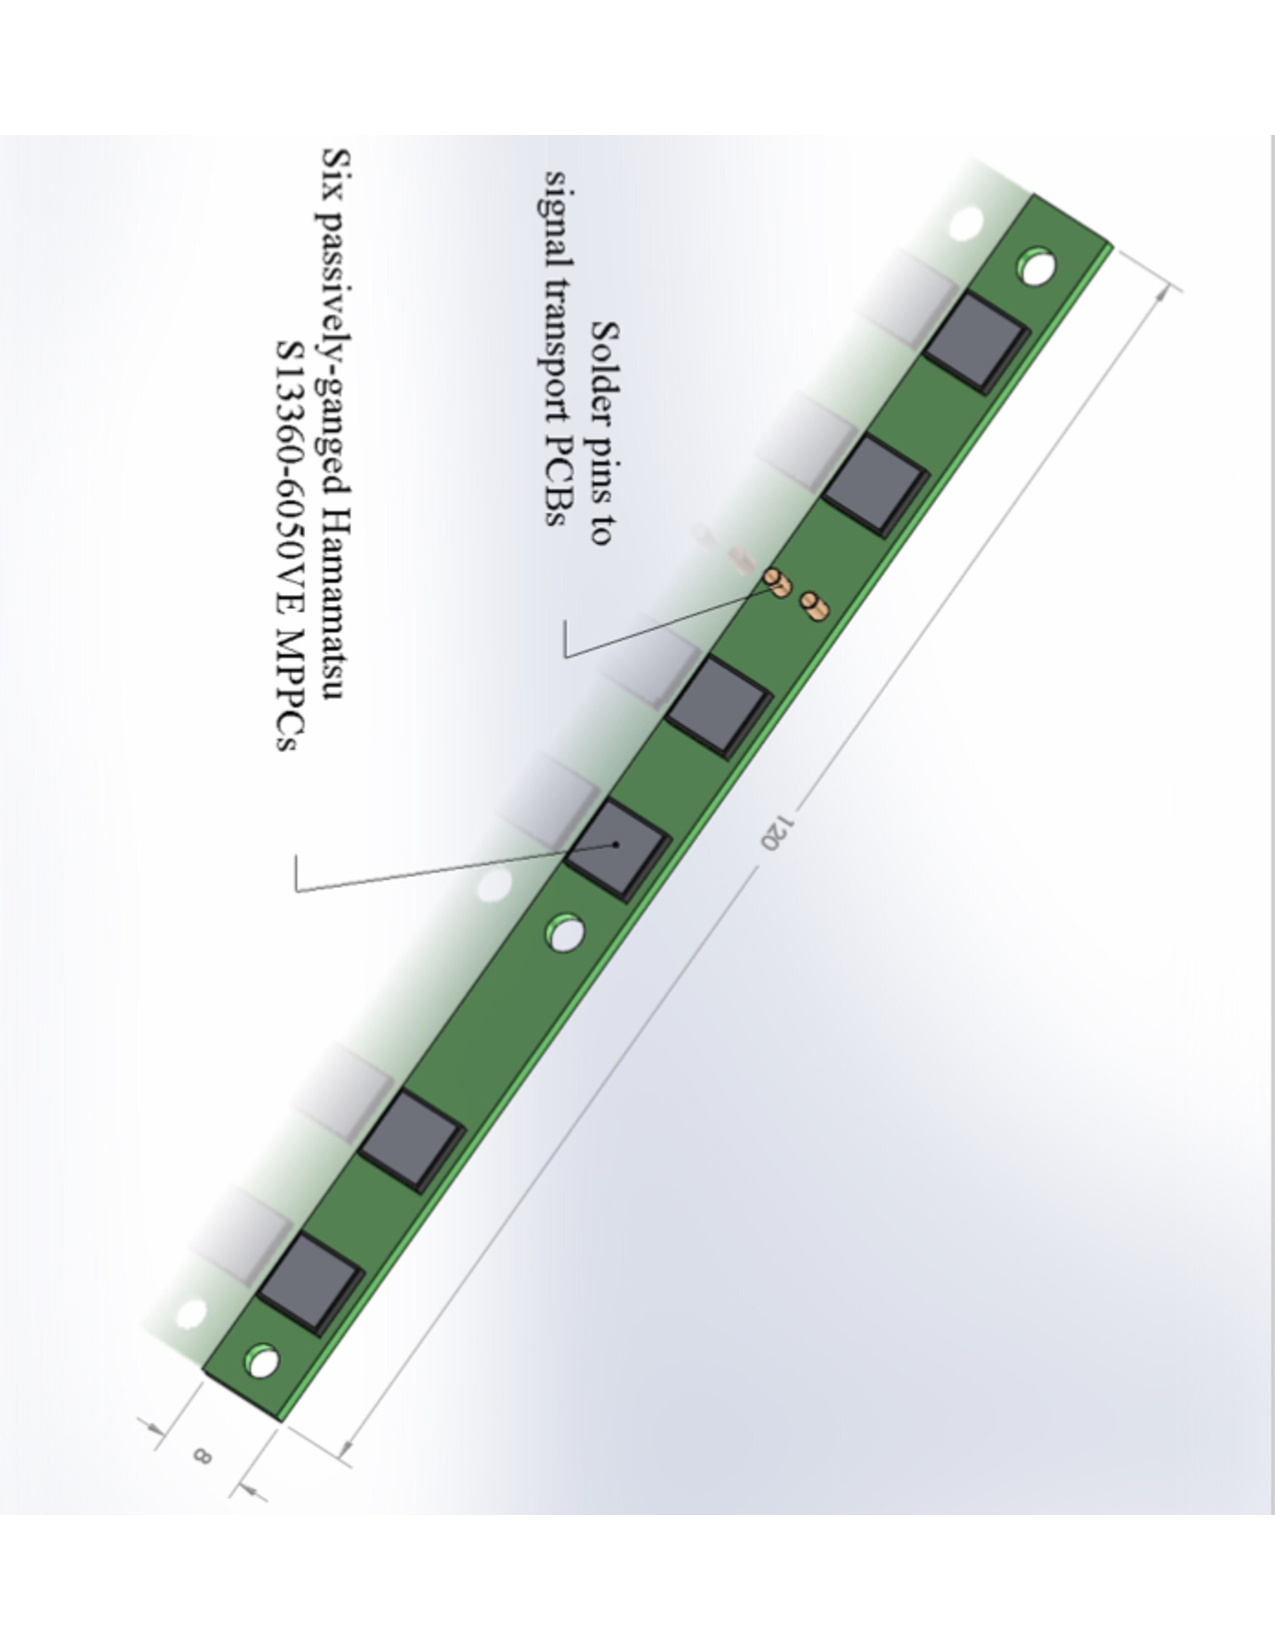
\includegraphics[angle=90,height=6cm]{pds-photosensor-mounting-board-r2}
  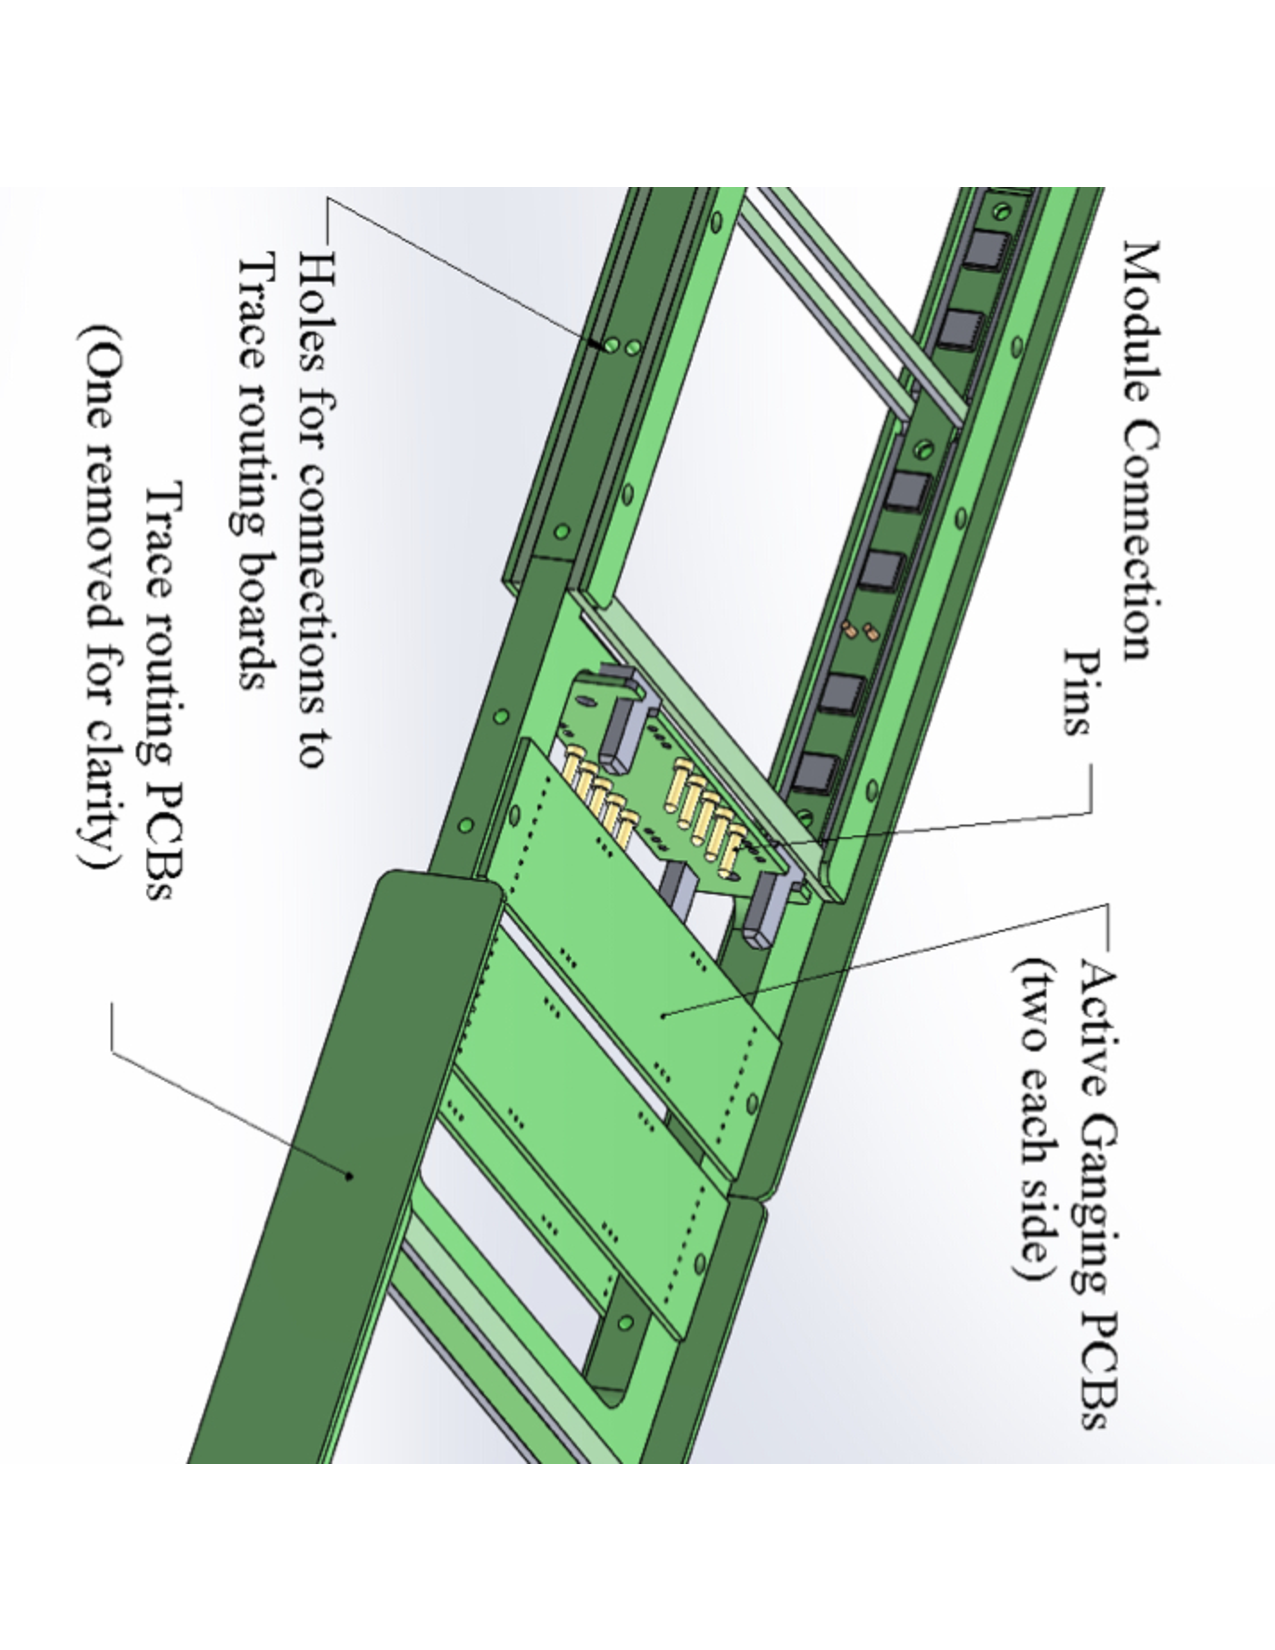
\includegraphics[angle=90,height=6cm]{pds-trace-routing-pcb}
\end{dunefigure}
The passively ganged signals are then routed through these boards to an active-ganging PCB at the center of the module, where all eight passively ganged signals from a single supercell are actively ganged into one output channel. This summed output from a single supercell is then connected to a single twisted pair in the cat-6 readout cable for the module.  The active ganging PCBs (one per supercell, four per module) are positioned in the module so that they are located inside the central APA mechanical support tube when fully installed.

%\fixme {add pictures of module center showing active ganging PCBs outside APA, and buried in central tube}

%\fixme{turned off figure for now--  it was killing my preview}

%\begin{dunefigure}[\dword{pdsp} ARAPUCA modules during assembly.]{fig:arap-prod01}
%{\dword{pdsp} ARAPUCA modules during assembly prior to installation of the dichroic filters; \dwords{sipm} and TPB coated reflector are visible.}
%  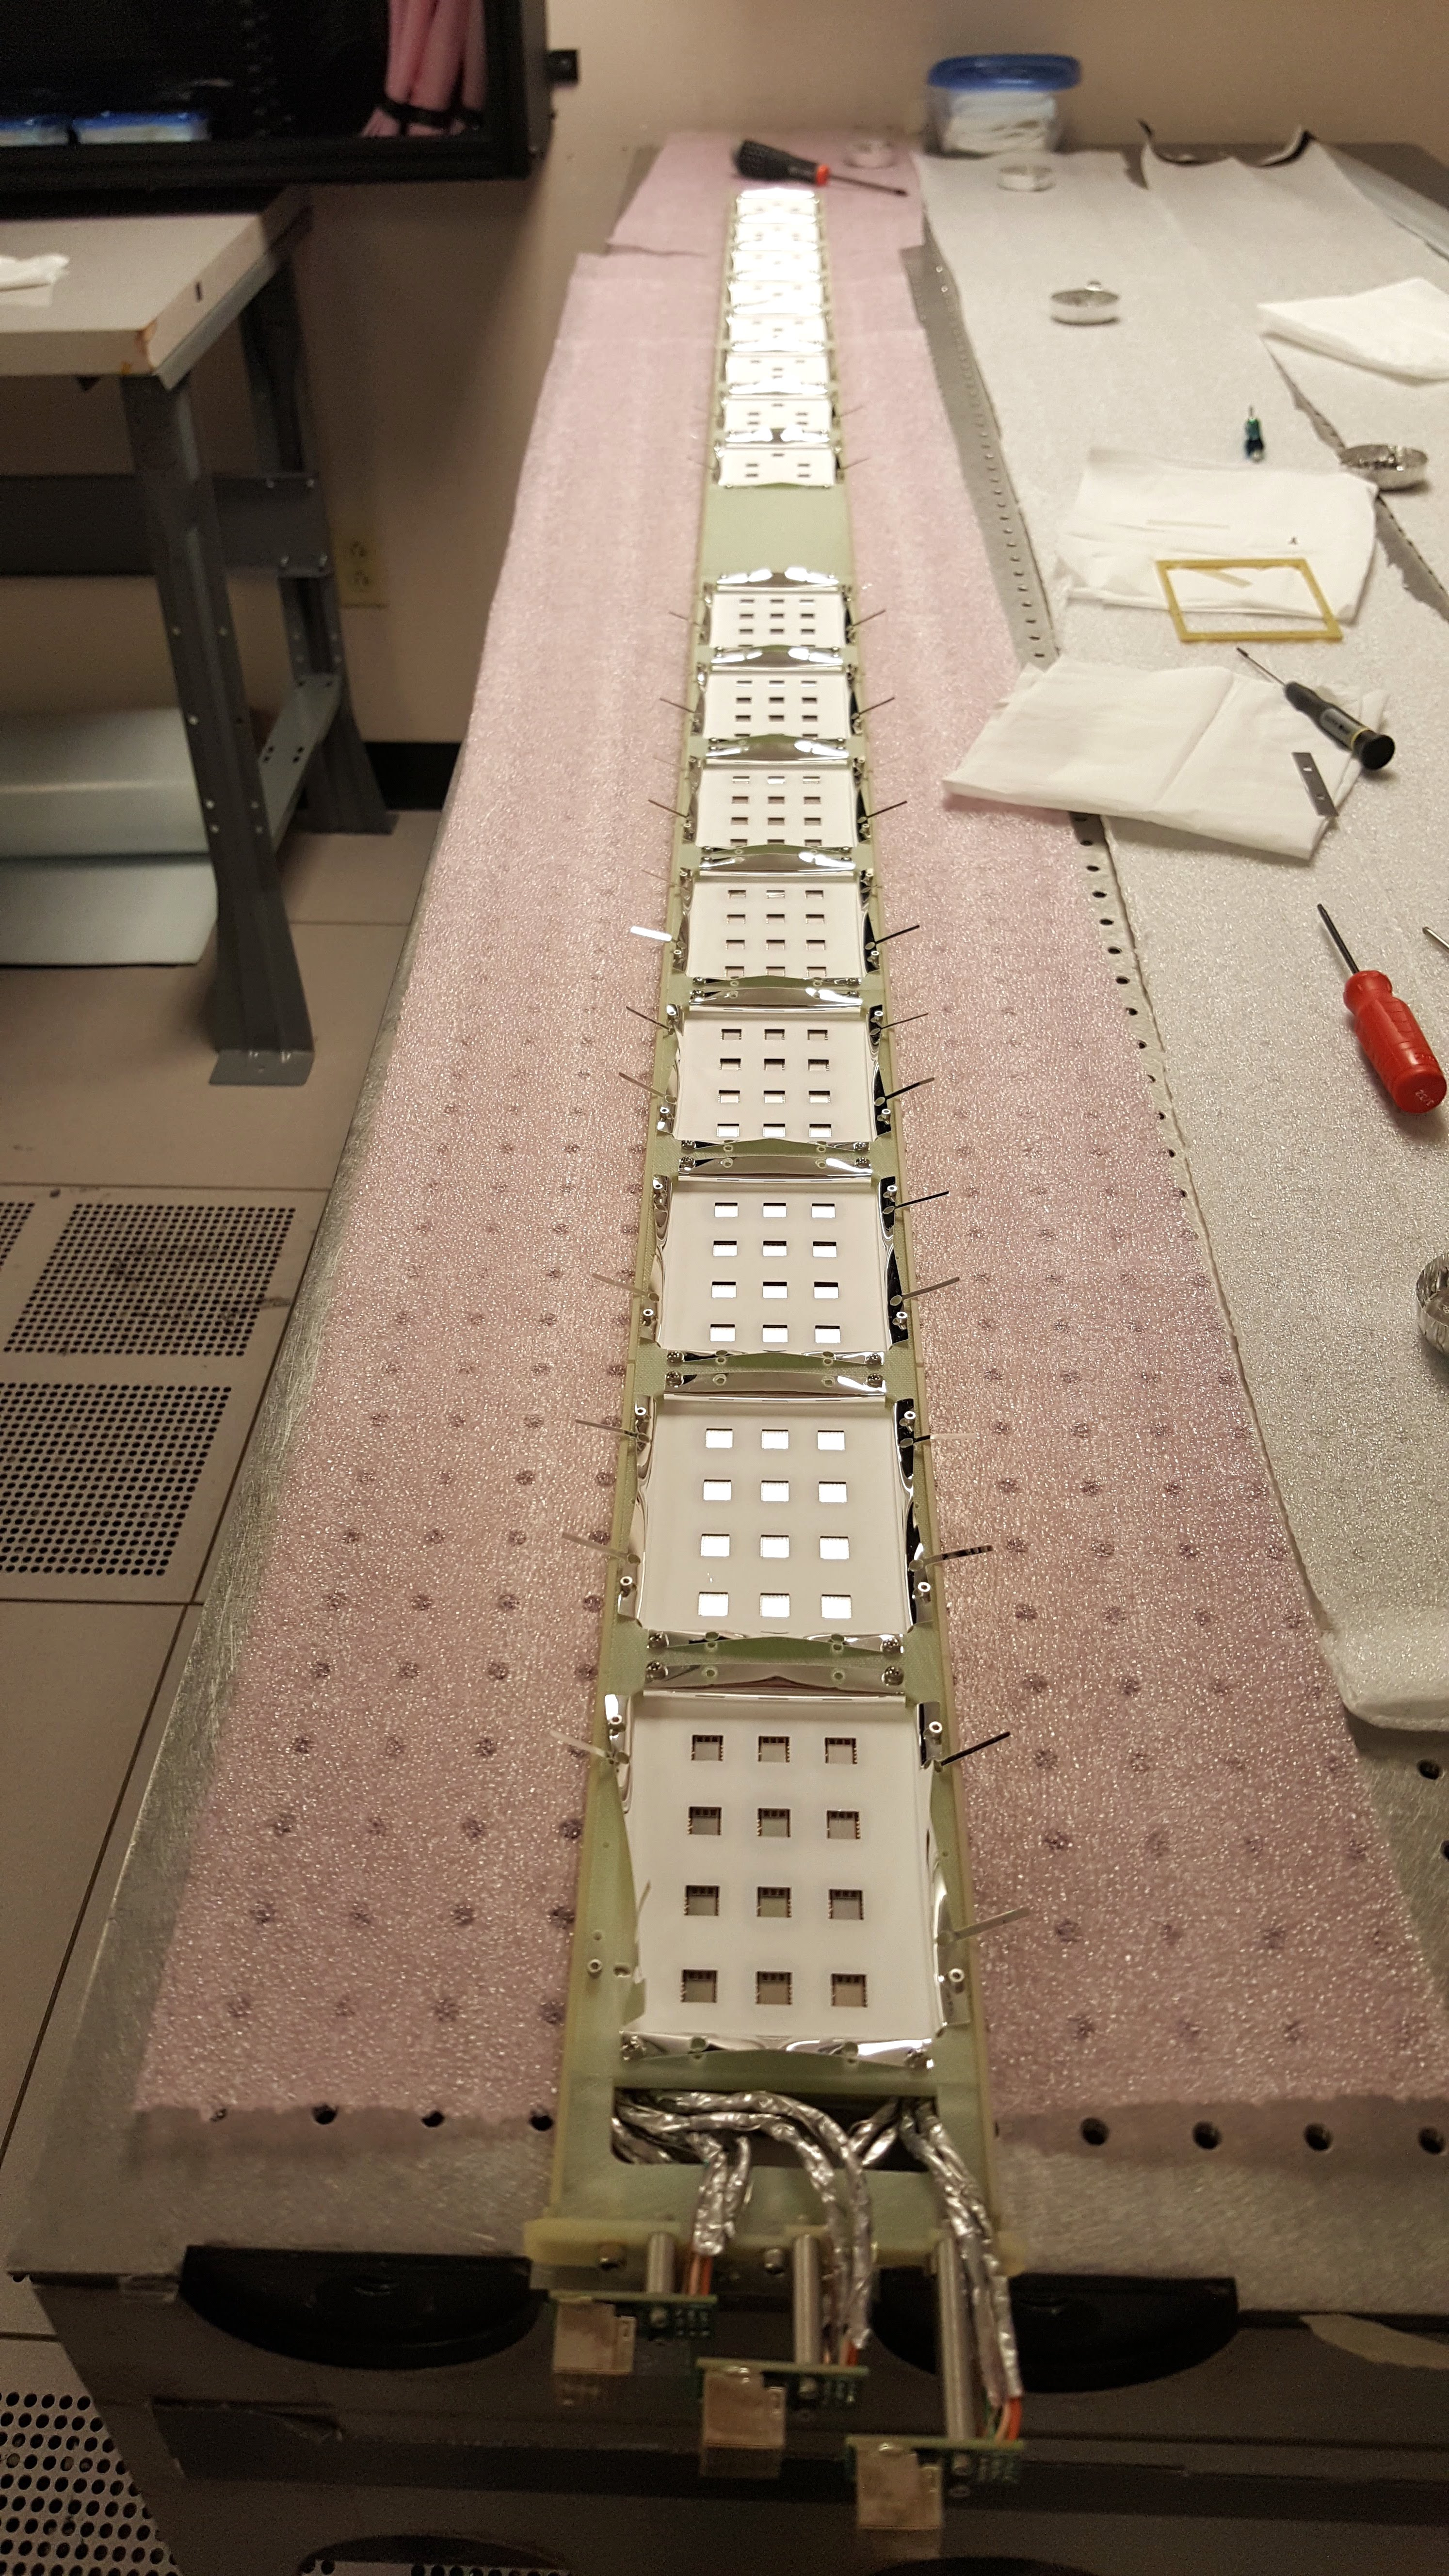
\includegraphics[height=8cm]{pds-arapuca-protodune02-apr18}
%\end{dunefigure}

The  internal surface of the sides the cell are lined with an adhesive-backed dielectric mirror foil\footnote{3M Vikuitiademar\texttrademark\  ESR - http://multimedia.3m.com/mws/media/193294O/vikuiti-tm-esr-application-guidelines.pdf} laser cut with openings at the locations of the \dwords{sipm}.  In the case of the single-sided readout the dichroic filter windows on the non-active side of the cell are replaced by a blank FR-4 G-10 sheet, lined in the cell interior with a Vikuiti\texttrademark\ reflector foil. %these are visible in Figure~\ref{fig:arap-prod01}, which shows an ARAPUCA during assembly prior to installation of the optical windows.

%The backplane \dword{sipm} boards for the \dword{pdsp} modules were designed at CSU and produced by an external USA vendor\footnote{Advanced Circuits Inc.; www.4pcb.com.}; the \dwords{sipm} were soldered on the boards using a reflow oven at CSU. Before mounting into the ARAPUCA module they were tested at room and LN2 temperatures. It is anticipated that the production of the boards for  \dwords{spmod} will be done outside the USA. %move to Brazil.
 %and the design will be optimized by Latin American institutions in collaboration with CSU.
%\fixme{want to specify Brazil?}

The optical window(s) of each supercell are dichroic filters with cut-off at \SI{400}{nm}. While the filters used for the \dword{pdsp} prototypes have been acquired from Omega Optical Inc.\footnote{http://www.omegafilters.com/}, other vendors are being considered for the DUNE production\footnote{ASHAI -Japan, Andover-USA, Edmunds Optics-USA}.
% rjw 12/2/18 the following moved to Prod and Assembly
%Prior to coating, the filters are cleaned according to the procedures given by the manufacturer using isopropyl alcohol. Since the most likely vector for scratching/damaging the coating is dragging contaminated wipes across the surface, new clean lint free wipes are used for each  cleaning pass on the surface. Clean filters are then baked at 100$^\circ$C for \SI{12}{hours}.    
   
The filters are coated on the external side facing the \lar active volume with pTP.  The coatings for the \dword{pdsp} modules have been made at the Thin Film facility at Fermilab using a vacuum evaporator. Each coated filter was dipped in LN2 to check the stability of the evaporated coating at cryogenic temperature. 
%For \dword{pdsp} \dword{pd} production the evaporation process will be performed at Unicamp in Brazil, where a large vacuum evaporator with an internal diameter of one meter is now available. The  conversion efficiency of the film deposited on the filters or on the Vikuiti\texttrademark\ foils will be measured with a dedicated set-up that will use the \SI{127}{nm} light produced by a VUV monochromator.
%\fixme{Bob:  I moved this to the assembly section  Dave: will this be done on every foil? Is this a design issue or QA/QC?}

%%%%%%%%%%%%%%%%%%%%%%%%%%%%%%%%%%%%%%%%%%%%%%%%%%%%%%%%%%%%%%%%%%%%%%%%%%%%
% rjw Moved the section on prototype measurements to the Validation section
%%%%%%%%%%%%%%%%%%%%%%%%%%%%%%%%%%%%%%%%%%%%%%%%%%%%%%%%%%%%%%%%%%%%%%%%%%%%


%==========================================================================================

%\fixme{Full light guides options sections removed - replace with summary, results and rationale for arapuca as baseline unless already addressed previously.}
%rjw 10/7/18 remove light-guide sections
%
%\subsection{Photon Collector: Dip-Coated Light Guides}
%\label{ssec:fdsp-pd-pc-bar1}
%\metainfo{\color{red} \bf Content needed: (4 pages) Toups}

%==========================================================================================


%%%%SILICON PHOTOSENSORS %%%%%%%%%%%%%%%%%%%%%%%%%%%%%%%%%%%%%%%%%%%%%%%%%%%

\subsection{Silicon Photosensors}
\label{sec:fdsp-pd-ps}
%\metainfo{\color{blue} Content update: Zutshi}

The \dword{spmod} \dword{pds} uses a multi-step approach to scintillation light detection with final stage of conversion into electrical charge performed by silicon photomultipliers (\dwords{sipm}). Robust photon detection efficiency, low operating voltages, small size and ruggedness make their use attractive in the \single design where the photon detectors must  %be accommodated
fit  inside the \dword{apa} frames. 

% rjw 12/1/18 Moved from the overview section
Based on extensive testing and experience with the vendor, we have selected a \SI{6}{mm}$\times$\SI{6}{mm} \dwords{mppc} %\dword{mppc} (Multi-Pixel Photon Counters) 
produced by Hamamatsu\footnote{Hamamatsu\texttrademark{} Photonics K.K., \url{http://www.hamamatsu.com/}.} (Japan) as the current baseline \dword{sipm} device. %including a model specifically designed for cryogenic operation. 
We are also vigorously pursuing an alternative based on the design of a device developed for operation in \lar by the DarkSide experiment collaboration and Fondazione Bruno Kessler (FBK)\footnote{Fondazione Bruno Kessler\texttrademark{}, \url{https://www.fbk.eu}.} (Italy).

The baseline \dword{pds} design has 192 \num{6}$\times$\SI{6}{mm$^2$} \dwords{mppc} per \dword{pd} module with groups of 48 \dwords{mppc} electrically ganged into four electronics readout channels. This leads to a total of 288,000 \dwords{mppc} per \dword{spmod}. The ganging (signal-summing) scheme is described in the next section.


%As implemented in \dword{pdsp}, there are twelve \num{6}$\times$\SI{6}{mm$^2$} \dwords{sipm} per bar and \numrange{6}{12} per ARAPUCA box.
%With this configuration, a \nominalmodsize \dword{spmod} with \num{150} \dwords{apa}, each with \num{10} \dword{pd} modules, would contain \num{18000}-\num{36000} (single or double-ended readout) \dwords{sipm} for the light guide designs and 10-20 times more for the higher granularity ARAPUCA design. This corresponds to approximately \num{1}-\SI{13}{m$^2$} of active \dword{sipm} surface area.

%% rjw 12/1/18 moved the "salient guiding principles" section to Design Considerations

%\fixme{update table - \dword{mppc} and FBK - remove other entries. In the text describe SensL since it was used in protoDUNE and give reason it is no longer a candidate.}

%\fixme{ rjw 11/25/18 reduce table to just Hamamatsu and up to two FBK device -- values to be inserted}
\begin{dunetable}[Candidate photosensors characteristics.]
{p{0.18\textwidth}p{0.18\textwidth}p{0.18\textwidth}p{0.18\textwidth}}
{tab:photosensors}
{Candidate Photosensors Characteristics.}
	                      &Hamamatsu (Baseline)   & Hamamatsu-2    & FBK                 \\ \toprowrule
Series part \#            & S13360                &     S14160         & NUV-HD-LF         \\ \colhline
Vbr (typical)                 & 50 V to 52 V          &   36 V to 38 V & 31 V to 33 V                \\ \colhline
Vop (typical)                 & Vbr + 3 V             &   Vbr + 2.5    & Vbr + 3 V                \\ \colhline
Temp. dependence          & 54 mV/K               &       35 mV/K      & 25 mV/K            \\ \colhline
Gain                      & $1.7 \times 10^6$     &      $2.5 \times 10^6$ &       $0.75 \times 10^6$          \\ \colhline
Pixel size                & 50 $\mu$m             &       50 $\mu$m    & 25 $\mu$m            \\ \colhline
Size                      & 6 mm x 6 mm           &     6 mm x 6 mm    & 4 mm x 4 mm            \\ \colhline
Wavelength                & 320 to 900 nm         &     280 to 900 nm  & 280 to 700 nm            \\ \colhline
PDE peak wavelength       & 450 nm                &        450 nm      & 410 nm            \\ \colhline
PDE @ peak                & 40\%                  &        50\%        & 50\%            \\ \colhline
DCR @ 0.5PE               & < 50 $kHz/mm^2$      & < 100 $kHz/mm^2$   & < 25 $kHz/mm^2$                \\ \colhline
Crosstalk                 & <3\%				  &      <7\%          & <3\%             \\ \colhline
Afterpulsing              &                       &                &                 \\ \colhline
Terminal capacitance      & 35 $pF/mm^2$          &   55 $pF/mm^2$     &      50 $pF/mm^2$           \\ \colhline
Lab experience            & Mu2e and DUNE prototypes      &                &     Darkside  \\         
\end{dunetable}


%\fixme{comment that result from ganging appear in the validation section another section}

%%%%ELECTRONICS %%%%%%%%%%%%%%%%%%%%%%%%%%%%%%%%%%%%%%%%%%%%%%%%%%%

\subsection{Electronics}
\label{sec:fdsp-pd-pde}
%\metainfo{\color{red}\bf  Content: Djurcic/Franchi/Moreno/Spitz/Toups}

%\subsubsection{Introduction}
%\label{sec:fdsp-pd-elec-intro}

%\fixme {rjw: 11/23/18 Zelimir: Editing section and correcting some wording.}

\fixme{It would be helpful to have a simple figure that shows the signal path - from SiPM to ganging to frontend electronics to DAQ indicating cable path lengths and location with respect to the APAs and cryostat.}

The \dword{pd} design requires the readout system to collect and process electrical signals from \dword{sipm}s reading out the light collected by the ARAPUCAs, an interface with the trigger and timing systems supporting data reduction and classification, and the ability to transfer data to offline storage for physics analysis.

As specified in Table~\ref{tab:spec:time-resolution}, the readout system must enable the T$_0$ measurement of non-beam events; this capability will also enhance beam physics by recording interaction time of events within 
beam spill to help separate against potential cosmic background interactions. A highly capable readout system was developed for use with \dword{pdsp} and prototype development as described in Section~\ref{sec:ssp-protodune-electronics}. However, a more cost-effective wave form digitization system developed for the Mu2e experiment has been identified and selected as the baseline choice. 

%Charge integration appears to be a likely candidate at this point in our development, as it offers the potential for a simpler, commercially available charge integration circuit and perhaps a smaller, less-expensive cable plant to read it out.  

% 12/3/18 Per Josh S  - the mu2e system can do this so can use for  this purpose. No need to reference the studies.
%Physics simulation studies are currently underway to determine if pulse-shape discrimination will be required, which would provide the capability to record both prompt and delayed components of scintillation light (characteristic times of \SI{6}{ns} and \SI{1.3}{$\mu$s}), the latter consisting mostly of single photoelectrons and thus place stringent requirements on signal-to-noise performance. 
%\fixme{Does the Mu2e system have this capability?}

In this section we first describe the scheme used to electrically gang the signals from 48 \dwords{sipm} followed by a description of the baseline frontend electronics system.

%The photon detector collects a limited amount of light, so it is desired to collect the light from both excited states.  
%Since this requirement has not yet been established the option is kept open in the electronics design.

%All light collector options require some level of electrical ganging of the \dwords{sipm}, either passive direct connection of the \dword{sipm} outputs or active (cold signal summing and possibly amplification).  To that end we desire a system where the ganging is maximized to minimize the electronics channel count while maintaining adequate redundancy and granularity, as well as readout system performance.  This represents a significant interface between the electronics, photosensor and light collector designs, and will be a main focus of our development and optimization work up to the \dword{tdr}.

%Selection of the ganging option will include passive or active solutions, where the active 
%circuitry may require cold components such as an amplifier in the \lar volume. Design options with active cold components will need 
%to address issues of power dissipation and potential risks of single-point failures of multi-channel devices inside the cryostat.
%In the case of passive ganging, analog signals are transmitted outside of the cryostat for processing and digitalization. 
%Successful demonstrations of passive ganging at \lar temperatures have been made for groups of four and twelve 6x6 mm Micro-FC-60035C-SMT C series, and groups of 2, 4, 8, and 12  Hamamatsu \dwords{mppc} (S13360-6050PE) at  \num{25}$^\circ$C, - \num{70}$^\circ$C and \SI{77}{K}. 
%Active ganging has been demonstrated for an array of 12 sensL \num{4}$\times$\num{4} arrays of \SI{3}{mm}$\times$\SI{3}{mm} sensL C-series \dwords{sipm} (48 in all) and  72 \dwords{sipm} mounted in a hybrid combination of passive and active ganging using \SI{6}{mm}$\times$\SI{6}{mm} \dwords{mppc} with a low noise operational amplifier--this design combines 12 active branches into the op-amp, where each branch has six \dwords{mppc} in a parallel passive-ganging configuration.

\subsubsection{SiPM Signal Ganging}
\label{sec:pds-design-ganging}
%\fixme{Zelimir added this subsection}

Photon collector techniques require electrical ganging of the \dwords{sipm} in order to maximize the active area of the photosensors while keeping the channel count reasonably low. The summing (ganging) of electrical signals from \dword{sipm} arrays is implemented to minimize the electronics channel count while maintaining adequate redundancy and granularity, as well as readout system performance.  Technical factors that affect performance of the ganging system are the characteristic capacitance of the \dword{sipm} and the number of \dwords{sipm} connected together, which together dictate the \dword{s/n} and affect the system performance and design considerations.

We have demonstrated a feasible passive summing scheme with twelve Hamamatsu \dword{mppc} sensors now operational in \dword{pdsp}. For optimal performance in DUNE, we have shown that an ensemble of 48 Hamamatsu \SI{6}{mm}$\times$\SI{6}{mm} \dwords{mppc} can be summed into a single channel by a combination of passive and active ganging (see Section~\ref{sec:pds-valid-ganging}).  In this scheme, an amplifier is used to adjust the \dword{mppc} output signal level to the input of an \dword{adc}; the active summing is realized with an OpAmp THS4131. This combination of passive and active ganging with cold signal summing and amplification is the baseline for the \dword{pds}.

\fixme{Need a figure with the circuit showing the DUNE 6 passive x 8 active configuration}

In addition to the baseline scheme, a parallel effort is underway to investigate further optimization including development of detailed simulation and testing of prototype boards in South America. One scheme being investigated simulates the signals of 12 passively ganged \dwords{sipm} passed through a charge integrator or a charge amplifier transimpedance model into a summing stage. The simulation flow and the simulated response are shown in 
%Figure~\ref{fig:fig-pds-gang-jorge-1}(left) shows design scheme used in the simulation flow presented in 
Figure~\ref{fig:fig-pds-gang-jorge-1}. Figure~\ref{fig:fig-pds-gang-jorge-2} shows the circuit designed based on these studies to be used with the \dword{pd} in the ICEBERG test stand (Section~\ref{sec:iceberg-teststand}).

\begin{dunefigure}[Active summing board design simulation flow.]
 {fig:fig-pds-gang-jorge-1}
 {Active summing board design simulation flow (left) and simulated response of the circuit with 48 \dwords{sipm}(right).}
% {The active summing board design scheme (left) used in the simulation flow (right).}
%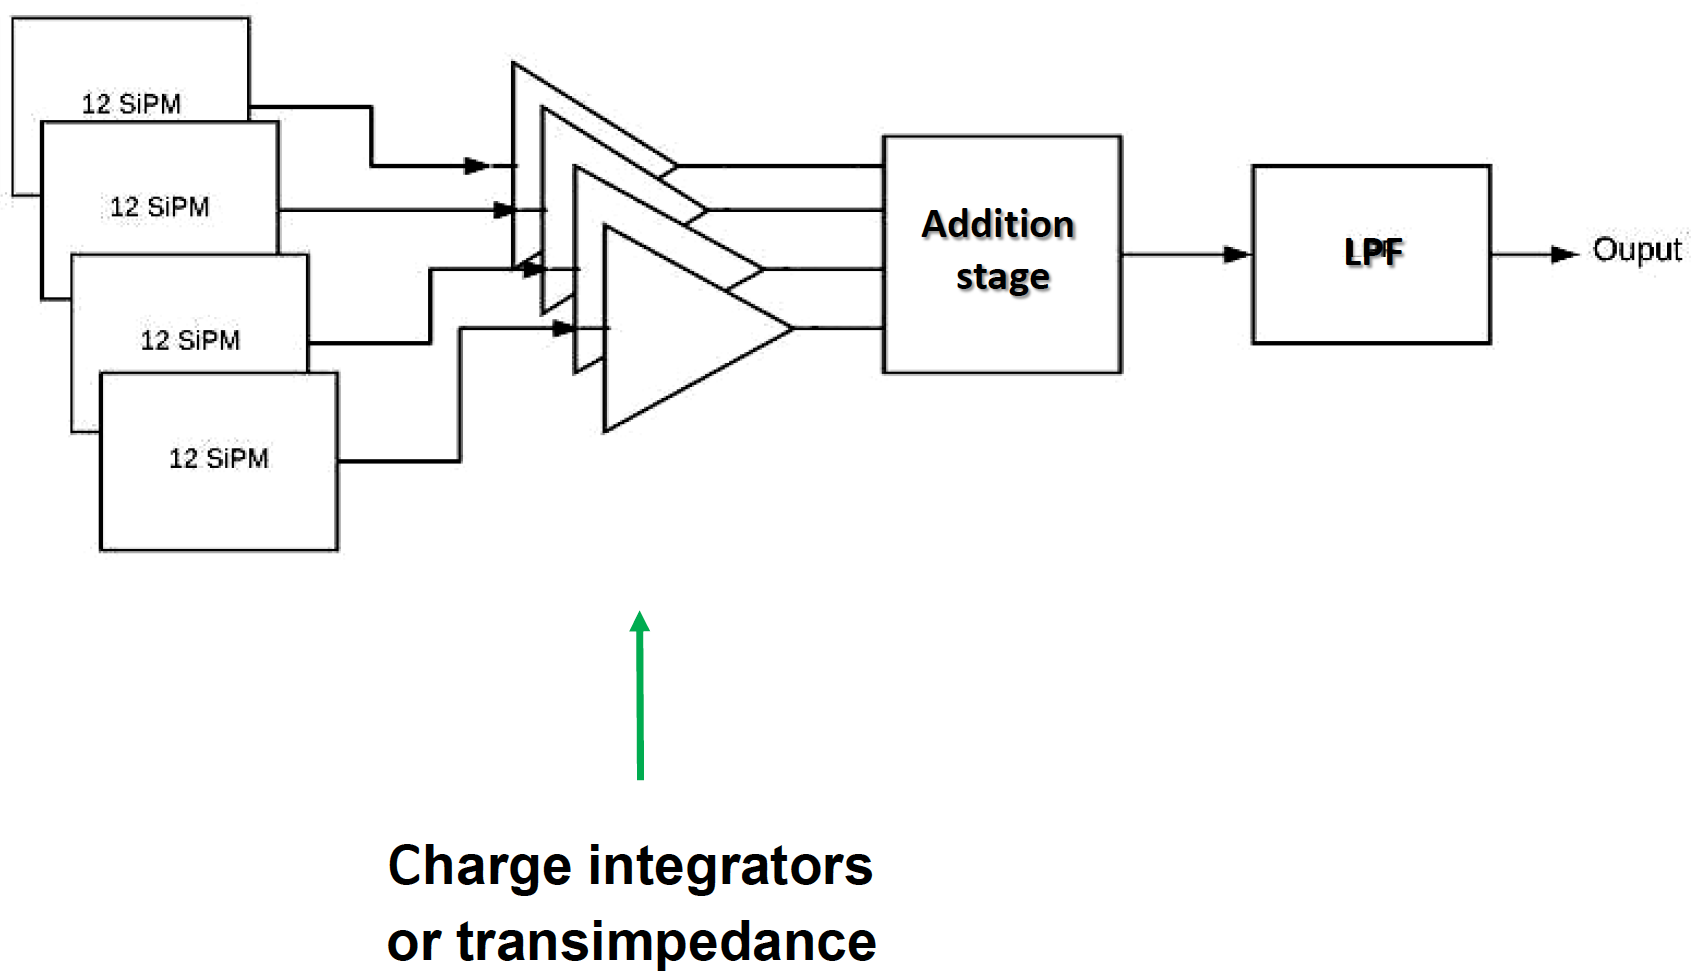
\includegraphics[angle=0,width=8.4cm,height=6cm]{graphics/pds-gang-jorge-1.png}
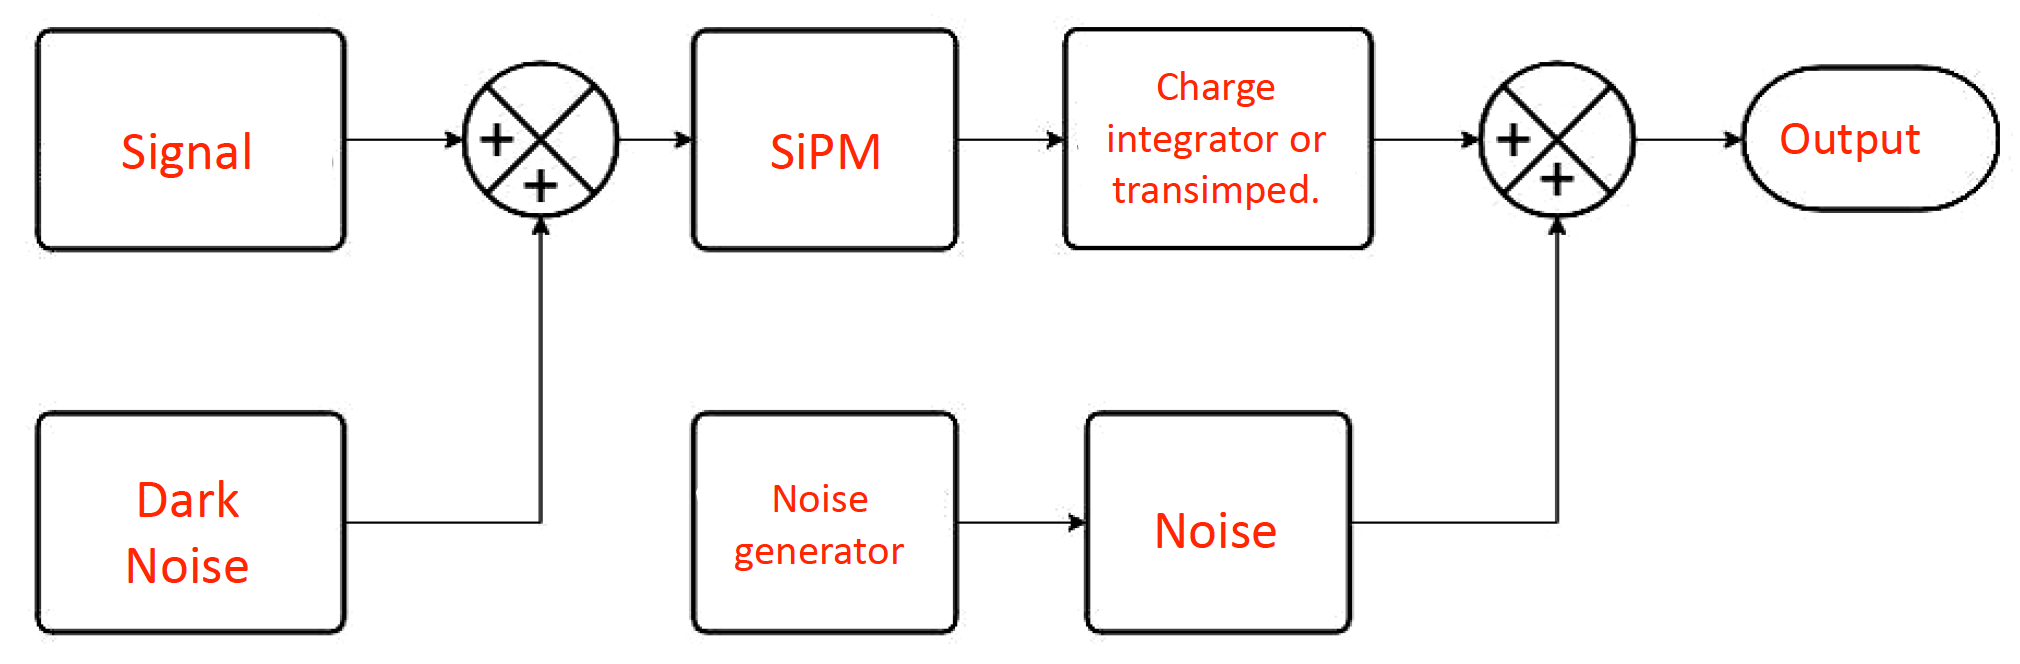
\includegraphics[angle=0,width=8.4cm,height=4cm]{graphics/pds-gang-jorge-2.png}
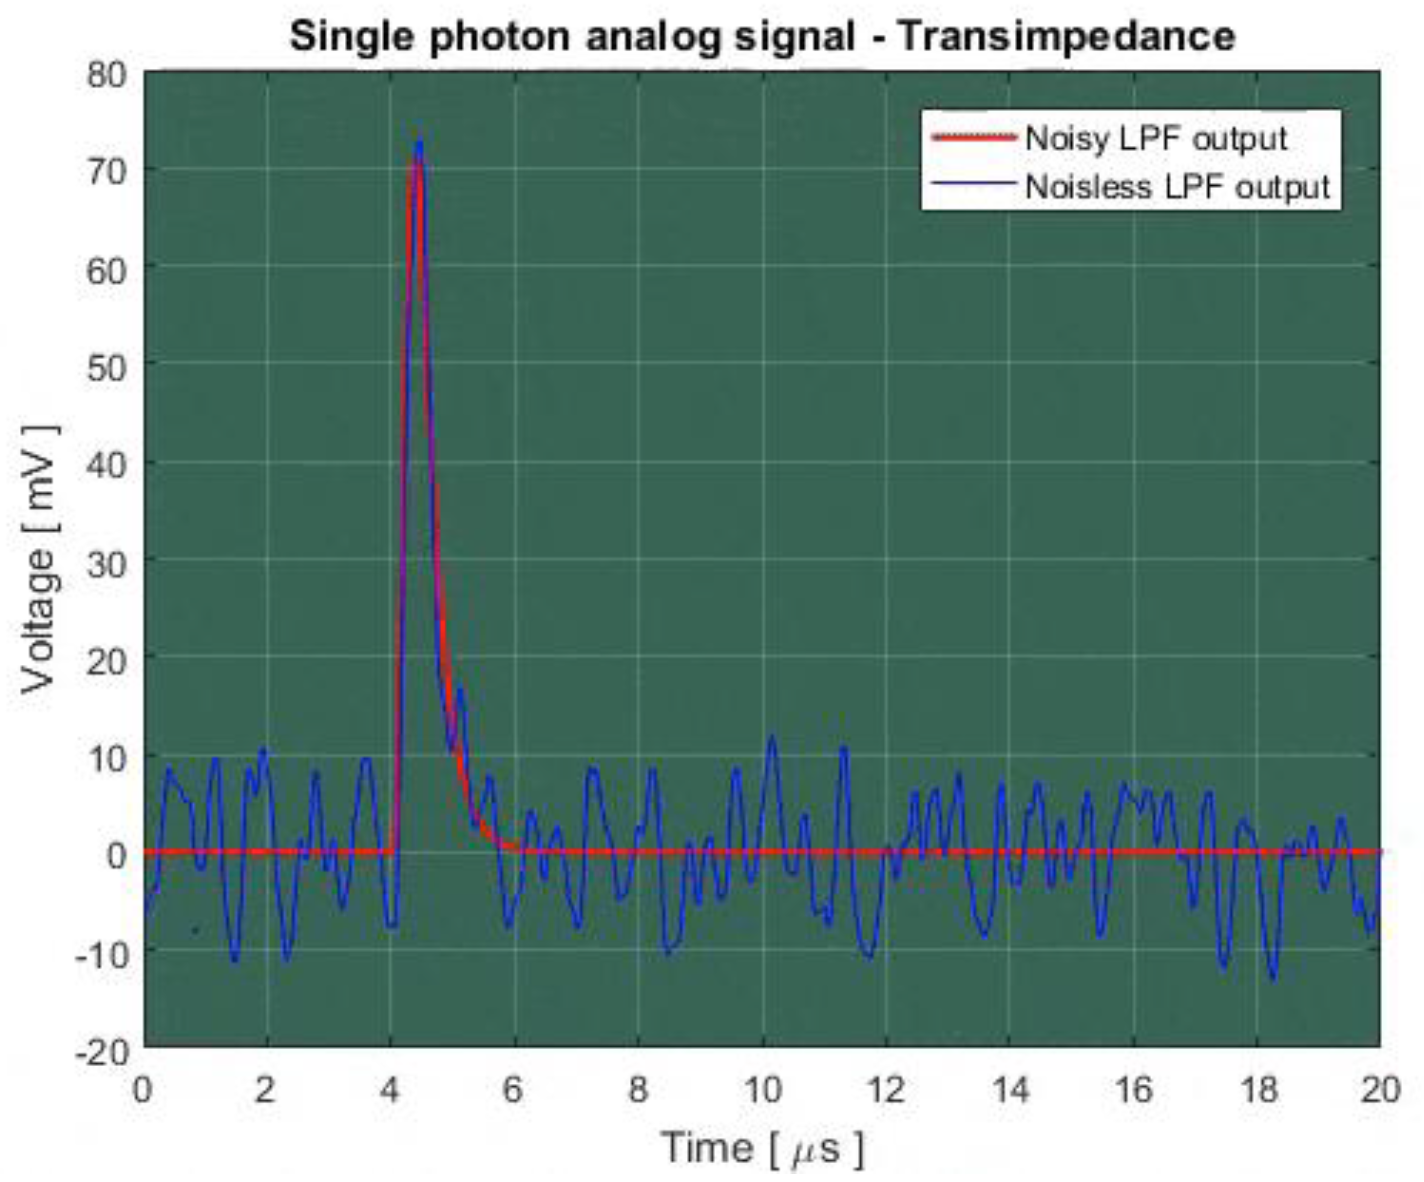
\includegraphics[height=4cm]{graphics/pds-gang-jorge-3.png}
\end{dunefigure}

\begin{dunefigure}[Active ganging circuit to be used in the ICEBERG test stand.]
 {fig:fig-pds-gang-jorge-2}
 {Active ganging circuit to be used in the ICEBERG test stand.}
%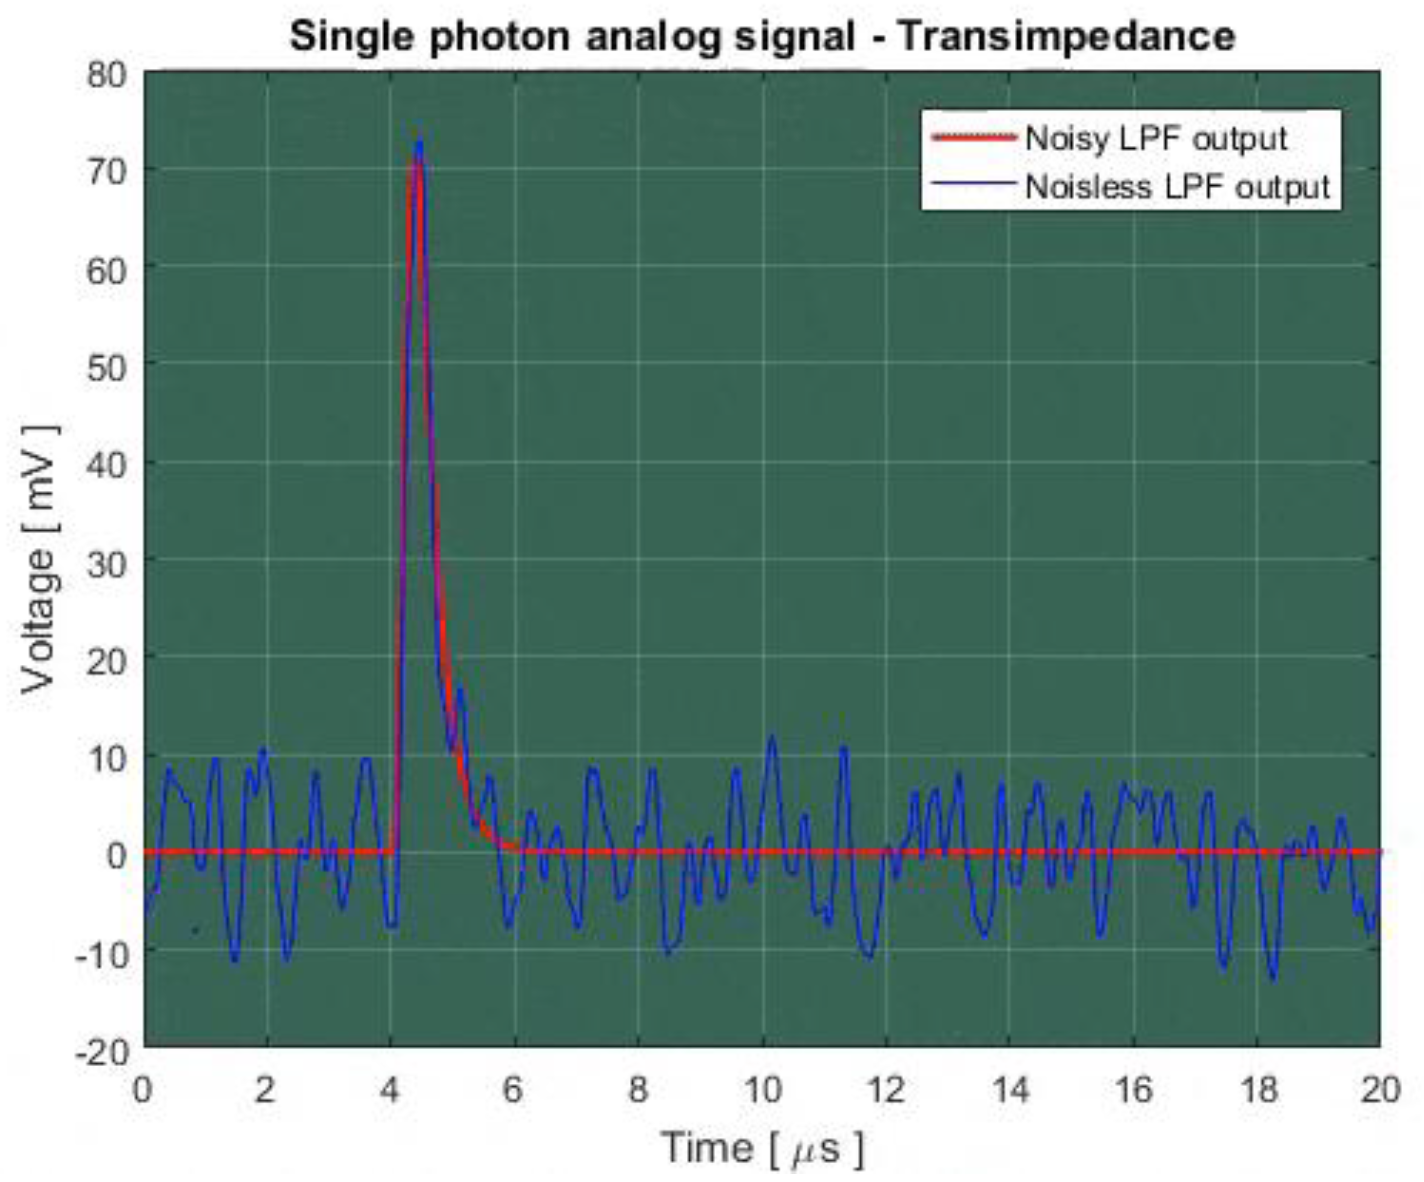
\includegraphics[angle=0,width=8.4cm,height=6cm]{graphics/pds-gang-jorge-3.png}
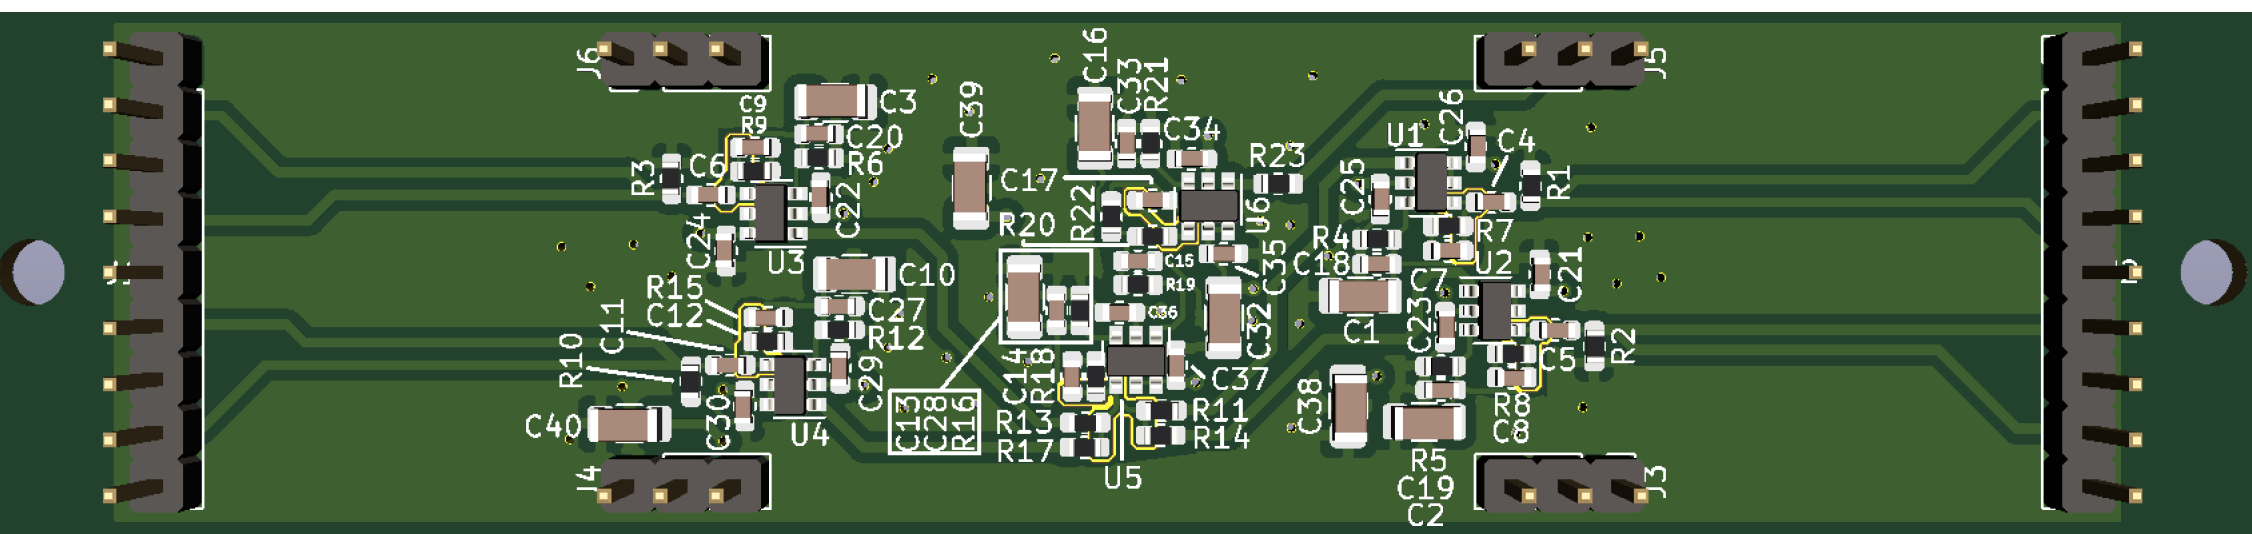
\includegraphics[angle=0,width=8.4cm,height=4cm]{graphics/pds-gang-jorge-4.png}
\end{dunefigure}

The development framework presented above presents a very powerful tool in the design of the electronics. It shows that is possible to gang 48 \dwords{sipm} and distinguish single photon signals with less than 1 $\mu$s width.
%.For single photons there is no significant difference between both models in duration of the pulse and S/N ratio. Preliminary simulations indicates that for 10 photons we don’t see any difference either.
The \dword{s/n} ratio obtained is about \SI{8}{dB}, with all noise effects, including thermal and dark noise contributions.

%\fixme{add more in validation section?}
%5.The optimal sampling rate obtained is >≈ 20 MSPS.
%6.The design of the board for the ICEBERG test stand is ready and in process of fabrication. It includes both designs in the same board, that can be easily exchanged.

%This solution is now used as the baseline summing option for DUNE Far Detector.
%next steps?:This board will also measure the photoelectron collection efficiency when the \dwords{sipm} are coated with \dword{tpb} as a reference for ARAPUCA measurements with a similar ganging level (the summing  board is the same size as the \dword{pdsp} ARAPUCA backplane to facilitate the comparisons). 

%Charge processing requires a charge preamplifier ideally located within the cold environment, so the design must take into consideration the failure risks and the power dissipated into the environment.

%\fixme{rjw 11/23/2018: Here should be a description of the Gustavo's and Paraguay groups ganging scheme options (results are in the validation section) - can we identify the FNAL scheme as baseline for the purpose of the TDR draft? Perhaps in the section add the circuit design and drawing of the ganging circuit board that could go in a 10kt production module.}
%\fixme{Zelimir added ganging from Gustavo, and from Jorge base on Jorge's 30\% review slides.}

%Typically, arrival time and total charge are the key parameters to be obtained from a detector. Extraction of these parameters 
%is possible using analog or digital systems. Charge preamplifiers will be connected to the output of the detector to integrate current producing a charge proportional output. 

% => this to next steps: In both systems, performance parameters related  to sampling rate, number of bits, power requirements, signal to noise ratio, and interface requirements should be evaluated to arrive to selected solution.  
%Pulse shapes can be fully analyzed to improve detection of a new physics but it will have an important impact on the digitalization frequency.

%********************************************************************************************%
%12/2/18 Dave/Gustavo/Jorge check?
%12/2/18 rjw The following was in the Prod and Assembly section but seemed more like a design issue.
% I have seen this discussed elsewhere so I will comment it out - Dave/Gustavo/Jorge should comment
%A basic level of active ganging locates summing circuitry on a separate PCB also mounted on the \dword{pd} module. A more complex scheme is being considered that would include cold amplifiers and ADCs. This solution would provide more flexibility in the level of photosensor ganging and also obviate the need for carrying analog signals of long cables. Production of the board would follow standards practices but the complexity introduces concerns with reliability and long-term stability issues related to cold electronics.  
%\fixme{Is this still being considered?}
%********************************************************************************************%



%%%%%%%%%%%%%%%%%%%%%%%%%%%%%%%%%%%%%%%%%%%%%%%%%%%%%%%%%%%%%%%%
\subsubsection{Front-end Electronics Baseline Design}
\label{sec:electronics}
%\fixme{11/28/18 I have pasted in Josh S. text/figures on Mu2e -- it needs integrating with the rest of the electronics section}

%%%%%%%%%%%%%%%%%%%%%%%%%%%
%rjw 12/1/18 following moved from the Considerations section since it is more Design choice.
Based on successful design, fabrication, operation and performance of \dfirst{ssp} readout in \dword{pdsp}, and with initial high-quality beam and cosmic ray day data collected by the \dword{pdsp} photon system, we are %have decided to 
further cost-optimizing the readout electronics.  To this end we have adopted a solution based on ultrasound ASIC chips rather than digitizers based on flash ADCs. Inspiration for %such a 
this cost-effective front-end comes from the system developed for the Mu2e experiment cosmic ray tagger readout system.
Both systems are currently used in the photon detector validation process summarized in Section~\ref{sec:fdsp-pd-validation}. The latter system 
\fixme{sounds like flash adc solution (the latter) is lower cost, but you're not using it. Is that right? (anne)}
performs a lower-cost waveform digitization based on the lower sampling rate commercial ASICs.
%and enables a thorough investigation of the photosensor signals, particularly as we investigate the impact of electrically ganging multiple \dwords{sipm}. 

%With the cost-effective front-end baseline based on ultrasound ASIC, the evolution of the readout electronics for the final system will be strongly influenced by the outcomes of \dword{mc} simulations that are in progress. Of particular interest is the extent to which pulse shape capabilities are important to maximizing sensitivity to low energy neutrino interactions from \dwords{snb}. 
%%%%%%%%%%%%%%%%%%%%%%%%

%\subsubsection*{Front-end board and controller}
\textit{\it Front-end Board and Controller}

The readout and digitization of the signals from the active summing board described in Section~\ref{sec:pds-design-ganging} will rely on a set of front-end board (FEB) readout electronics boards and controller boards, originally designed for the Mu2e experiment~\cite{bib:mu2e_tdr} %by the Electrical Engineering Department 
at Fermilab. As discussed in Section~\ref{sec:pds-valid-ganging}, preliminary results indicate that the active-summing board and Mu2e electronics FEB combination will perform well together and, in general, meet the readout requirements for the experiment. The 64~channel FEB design carried over from Mu2e can be seen in Figure~\ref{fig:feb}. The board has a number of notable features, discussed below. Most importantly, %however, 
the board is designed to utilize commercial, off-the-shelf parts only, and is therefore quite inexpensive compared to other designs. In particular, we will use low-noise, high-gain, and high-dynamic-range commercial ADCs used in ultrasonic transducers %are being used 
for the digitization.

The FEB is the centerpiece of the baseline readout electronics system. %envisioned. 
The current 64~channel\footnote{This text assumes 64 channels/FEB when presenting the FEB and controller. However, we envision 40~channels/FEB in the final design, corresponding to a single APA as described in the ``Next Steps" section.} FEB relies on commercial ultrasound chips (12~bit, 80~MS/s; AFE5807 by Texas Instruments),
fixme{footnote needed with TM}  with programmable anti-alias filters and gain stages, to read out the \dword{mppc} signals from the active ganging boards inside of the detector modules. The board currently takes HDMI inputs, with four channels per input.  Each of the eight ultrasound chips on an FEB handles eight channels (\SI{120}{mW} per channel) of data using a low-noise preamplifier, a programmable gain amplifier, and a programmable low-pass filter. The information is buffered with a total of \SI{1}{GB} DDR SDRAM, divided in four places, and a set of Spartan~6 FPGAs are used for parallelizing the serial \dword{adc} data, zero suppression, and timing. Each of the four FPGAs on a board, corresponding to 16 channels, handles two ADC chips with an available \SI{256}{MB} DDR SDRAM. 

After digitization, the data from each FEB, in the form of pulses (time-stamp and pulse height) is sent to a master controller via ethernet, which aggregates the signals from 24 FEBs, or $64 \times 24=1536$ channels. The 24 FEBs corresponding to a single controller will come in sets of 12, with each set of 12 FEBs referenced to a single chassis. A picture and schematic of the controller is seen in Figure~\ref{fig:controller}. A trigger decision can be produced and/or received (e.g., accelerator timing signal) by the controller and, depending on the decision, each event's digital information is sent to the controller and then to \dword{daq} computers for processing and storage. The controller-to-\dword{daq} connection will rely on a fiber connection, although an ethernet-based controller output option is available.

% \fixme{Since we cannot use this feature (next paragraph) is it worth mentioning? would it need to be removed by the redesigned FEB? Is that step scheduled?}

% In addition to its digitization and decision-making abilities, the current FEB has a number of other notable features. For example, each FEB contains an onboard Cockcroft-Walton (CW), which is available to generate bias voltage for the \dwords{mppc}. Notably, however, the CW is not currently considered an option for the summing board as it isn't stable enough to bias the differential amplifier. The CW is capable of providing $\approx$+75 V of bias. The board can also apply $\approx$-3~V to the \dword{mppc} anode, allowing the possibility of 78~V. In addition to the \dword{mppc} bias, the FEBs allow for an on-board current measurement (\SI{100}{pA} resolution) for producing IV curves of \dwords{mppc}. The FEBs can also be used in stand-alone mode, without a controller, via a telnet interface, which is useful for R\&D purposes and debugging. 
 
\textit{\it Bandwidth, readout rates, and zero suppression}

\dword{daq} system and data storage limitations impose constraints on the the data flow from the front-end electronics system. 
For example, if it was necessary to read out a 5.5~$\mu$s waveform (which represents the longest reasonable waveform 
%is 5.5 mus based on simulation? What happens with overlaping waveforms where longer readout is required, plus calibration etc?
in order to include late-light), the 80~MS/s, 12 bit ADC device would produce a 5.3~kbit waveform. For an envisioned dark count (DC) rate of 250~Hz/channel, this corresponds to a data transfer rate of 53~Mbps/APA (1~APA=40 channels) or 6.6~MB/s FEB-to-controller DC rate. This rate is approaching the crucial bottleneck in the electronics readout system that has a maximum 10~MB/s FEB-to-controller rate (per FEB). However, zero suppression techniques and multi-channel coincidence/threshold requirements at the FEB firmware level can be used to significantly mitigate this issue, noting that each on-FEB FPGA handles 16 channels. 

It will be necessary to fully understand the system requirements such as the suppression factor in terms of parameters like the readout window length and overall trigger rate to guide the final design. 
Firmware and zero suppression technique development is in progress and will be informed by the physics and calibration requirements of the detector. 
% \fixme{I didn't quite understand this next paragraph - could you rephrase?}
%In addition to its bandwidth and readout capabilities in consideration of DC rate as a concrete example,
In addition to its bandwidth and DC rate readout capabilities, the system is also capable of managing a highly-coincident event in which a large number (or all) channels fire at once. For example, a ``maximum (unrealistic)" all-detector event featuring 6000~channels firing at once (corresponding to 4~MB) could be handled by the controller's 24-board write speed of 150~MB/s. 

The baseline electronics readout system performance is consistent with the DAQ interface specification of 8~Gbps per connection as well, since each FEB signal corresponds to a maximum of 10 Mbps (240 Mbps total).  

\textit{\it Power, grounding, and rack schemes} 

The grounding, power, and data link schemes for the system are shown in Figure~\ref{fig:grounding_power}. The FEBs are powered via power-over-ethernet (600 mA, 48 V supply) from the controller. One Cat-6 cable from the controller to each FEB handles the signal and power simultaneously. The reference planes of the controller and FEB are isolated on both sides. The grounding scheme calls for each set of 12 FEBs referenced to a single chassis, with each chassis and corresponding controller on detector ground and the DAQ, connected to each controller via fiber, on building ground. 
 
The rack space and power consumption required by the system is based on a 6000 channel total assumption with 40 channels/FEB: this system requires 13 chassis (12 FEB/chassis) at 6u each and 7 controllers (controlling 24 FEB each) at 1u each. Assuming 42u per rack and with this requirement of $\approx$85u, just over 2~racks are needed. The power supply on a controller is 700~W, with each FEB taking 20~W. 
 

\begin{dunefigure}[64-channel \dword{pds} front-end board (80~MS/s, 12 bit)(left).]
 {fig:feb}
 {A picture of the 64-channel \dword{pds} front-end board (80~MS/s, 12 bit)(left); schematic of the front-end board (right).}
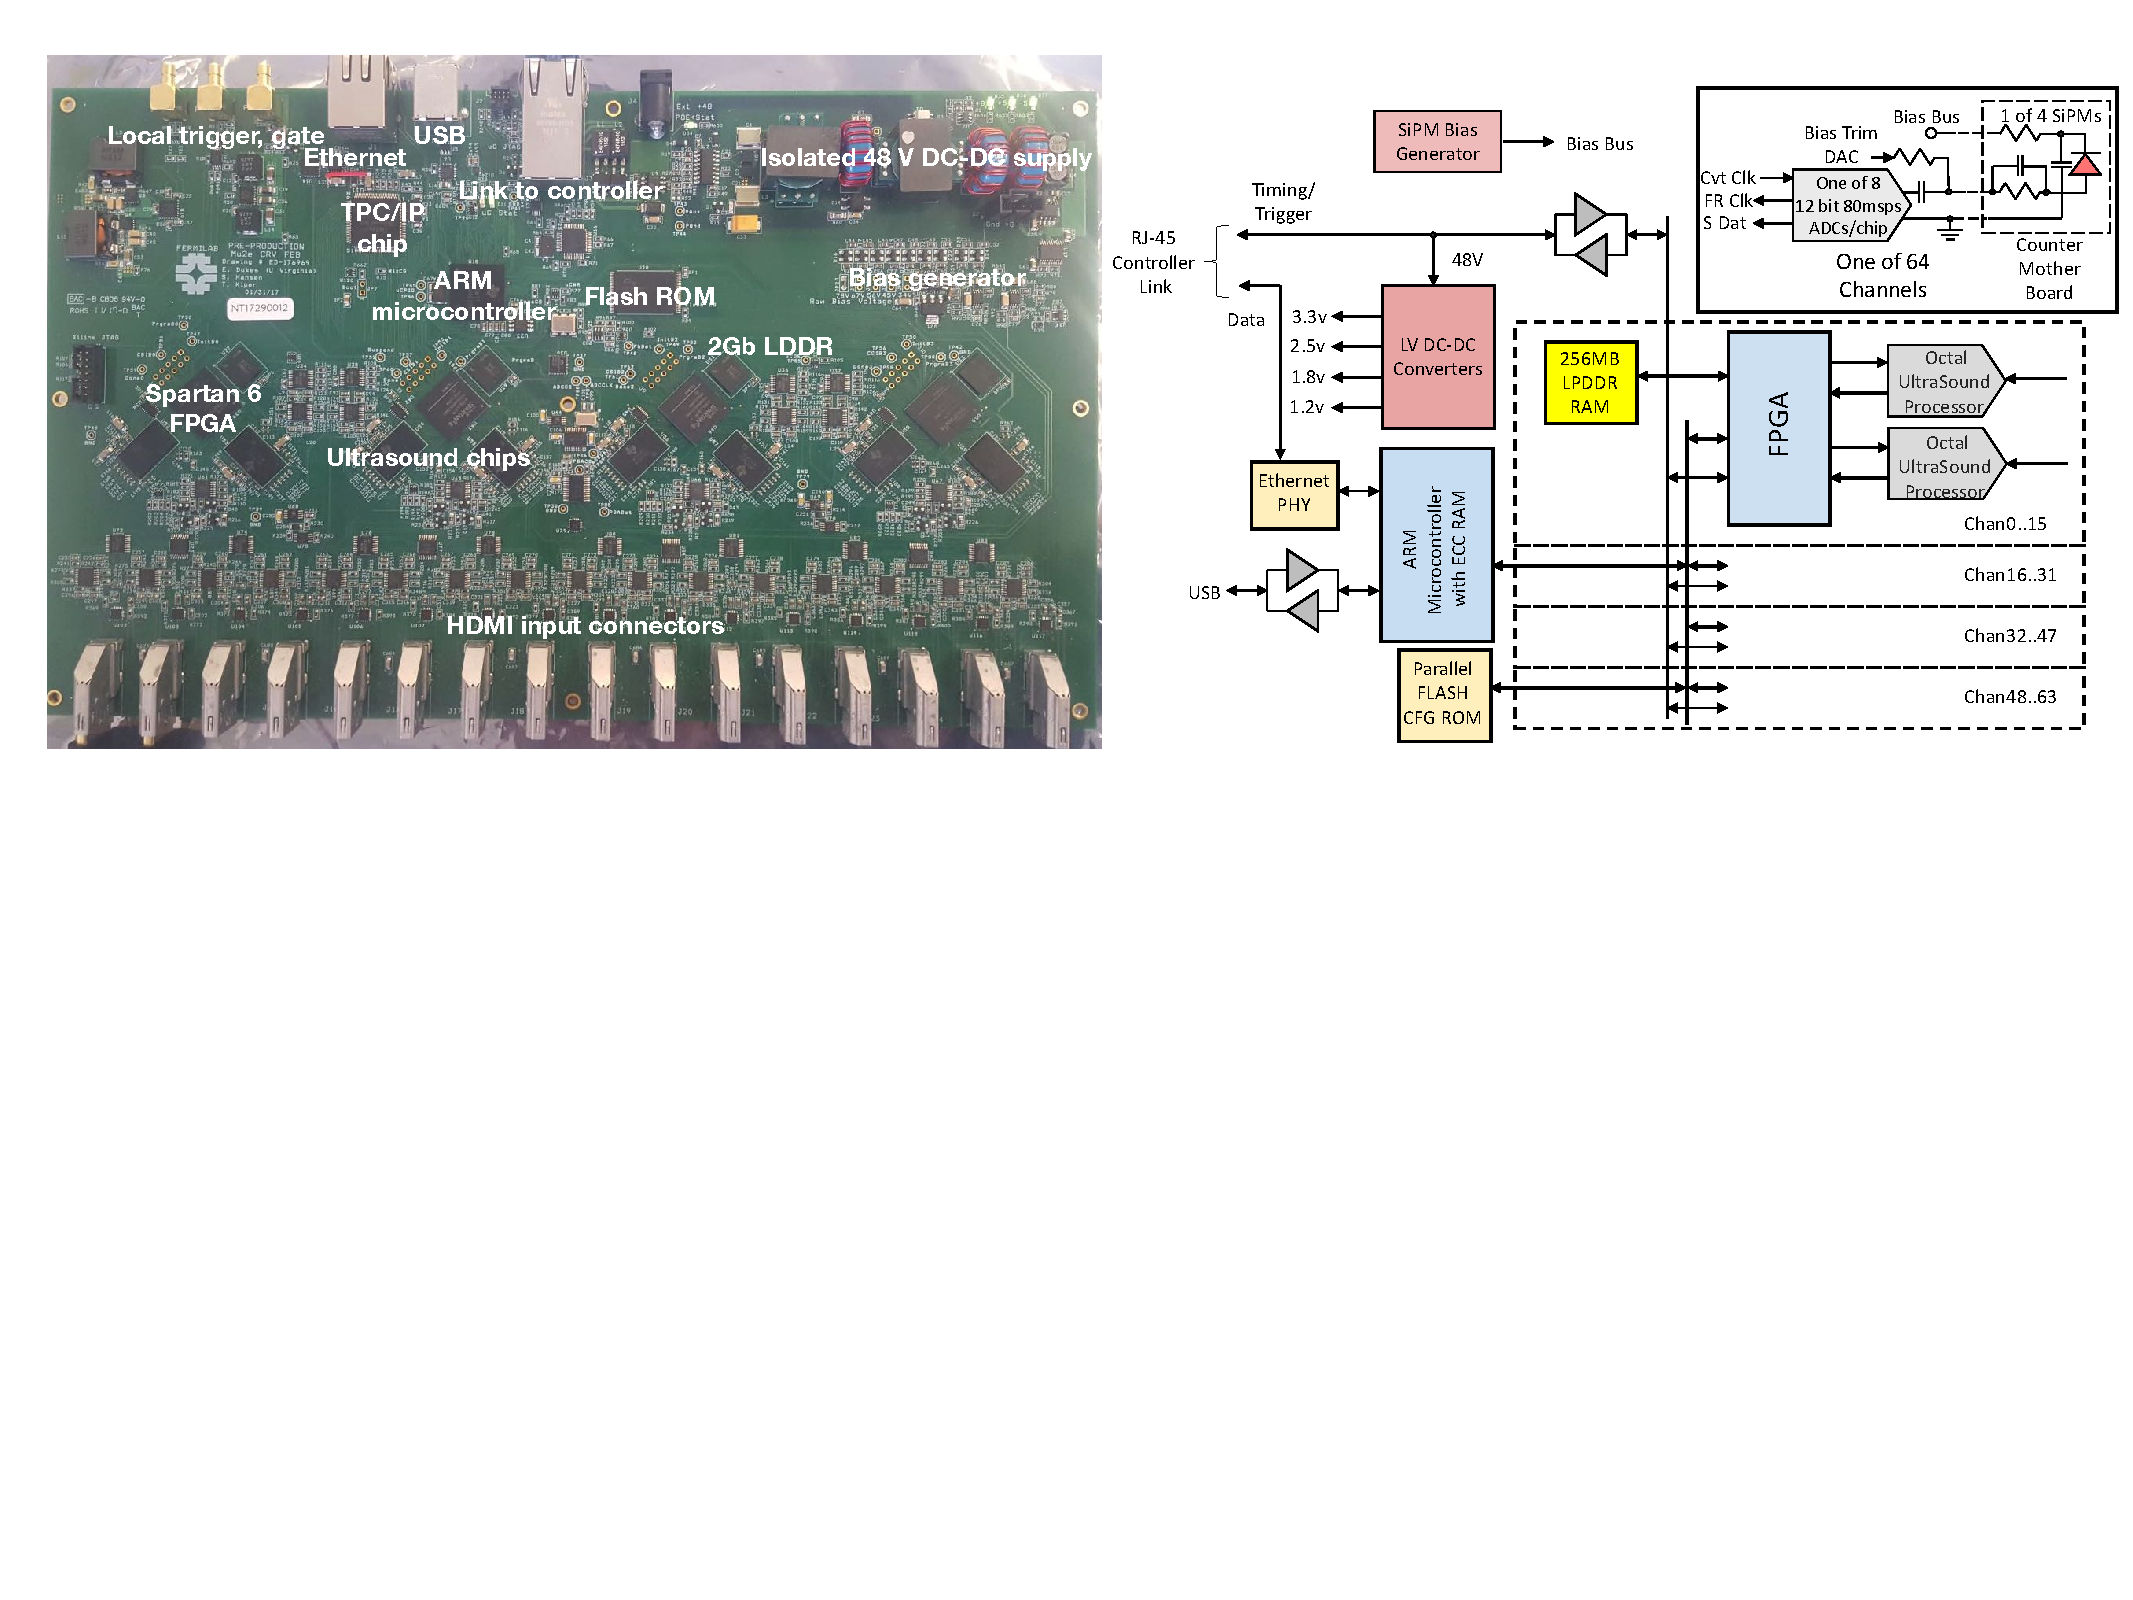
\includegraphics[height=4.8in]{graphics/pds-feb-tdr.pdf} 
\vspace{-6.3cm}
\end{dunefigure}

% \fixme{Need separate PDF for the board photo and schematic in this figure.}

%\begin{figure}
%\begin{centering}
%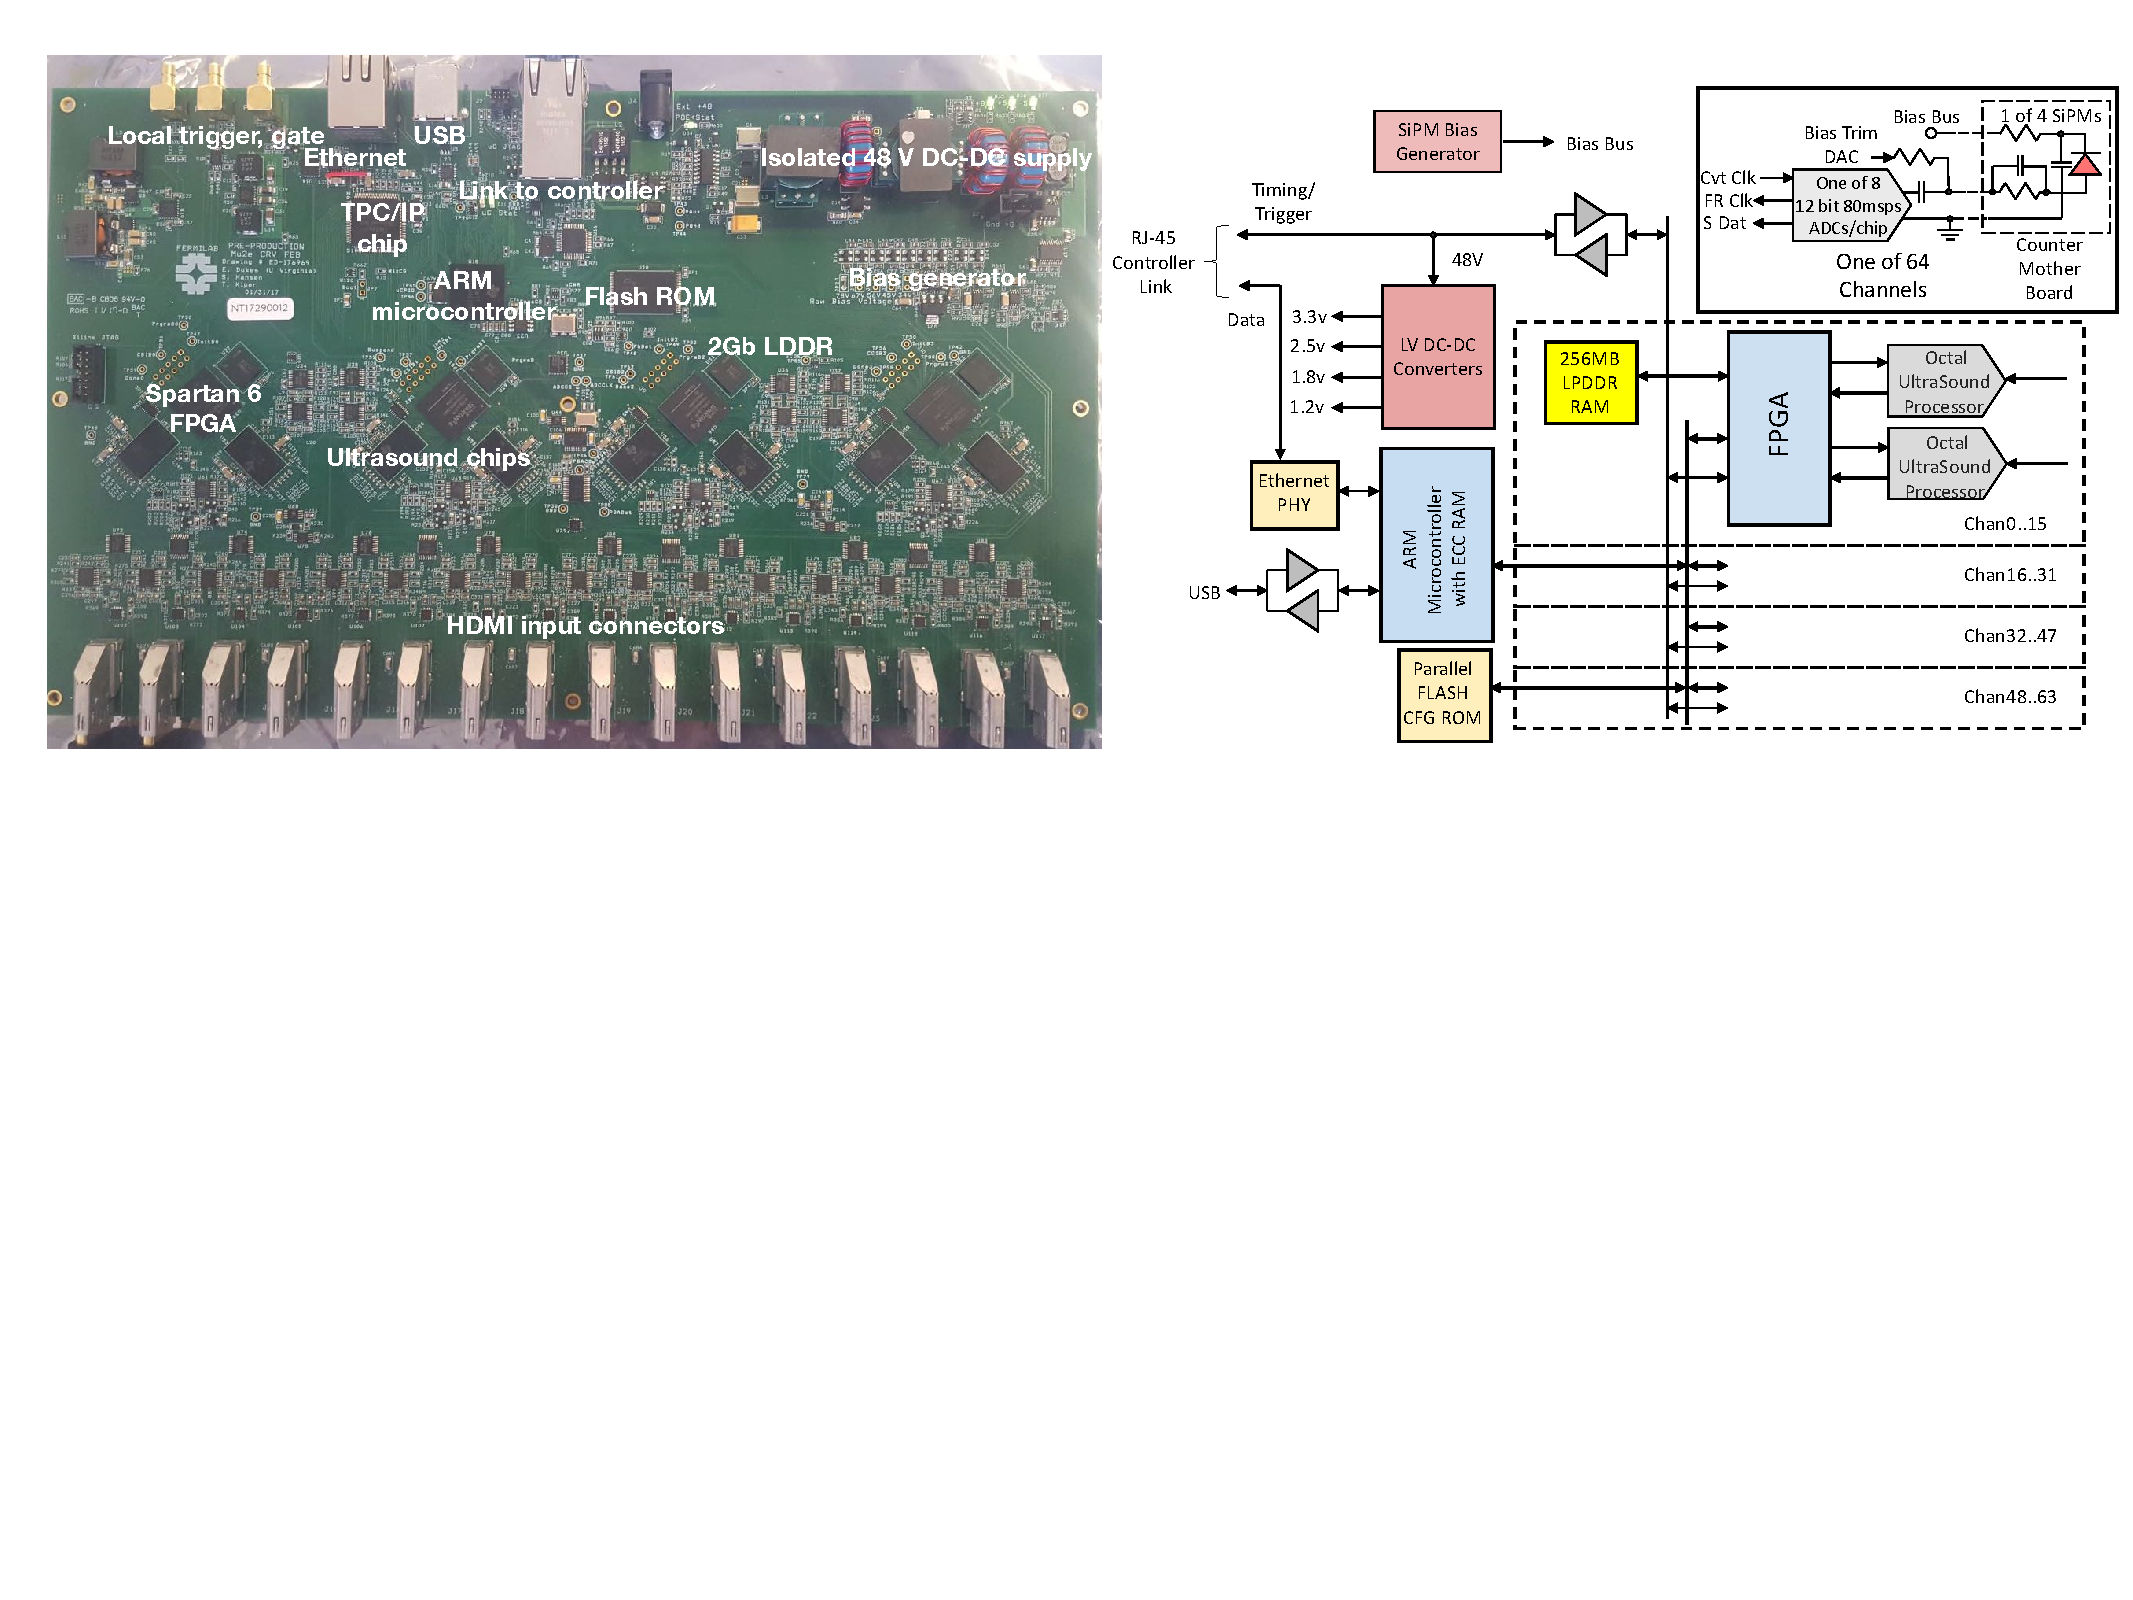
\includegraphics[height=4.8in]{graphics/pds-feb-tdr.pdf} 
%\vspace{-6.3cm}
%\caption{A picture of the 64-channel \dword{pds} front-end board (80~MS/s, 12 bit)(left); schematic of the front-end board (right).}
%\label{fig:feb}
%\end{centering}
%\end{figure}

\begin{dunefigure}[\dword{pds} front-end electronics controller module.]
 {fig:controller}
 {The front (left-bottom) and back views of the controller module (left-top), which is capable of accepting signals from 24 FEBs; schematic of the controller (right).}
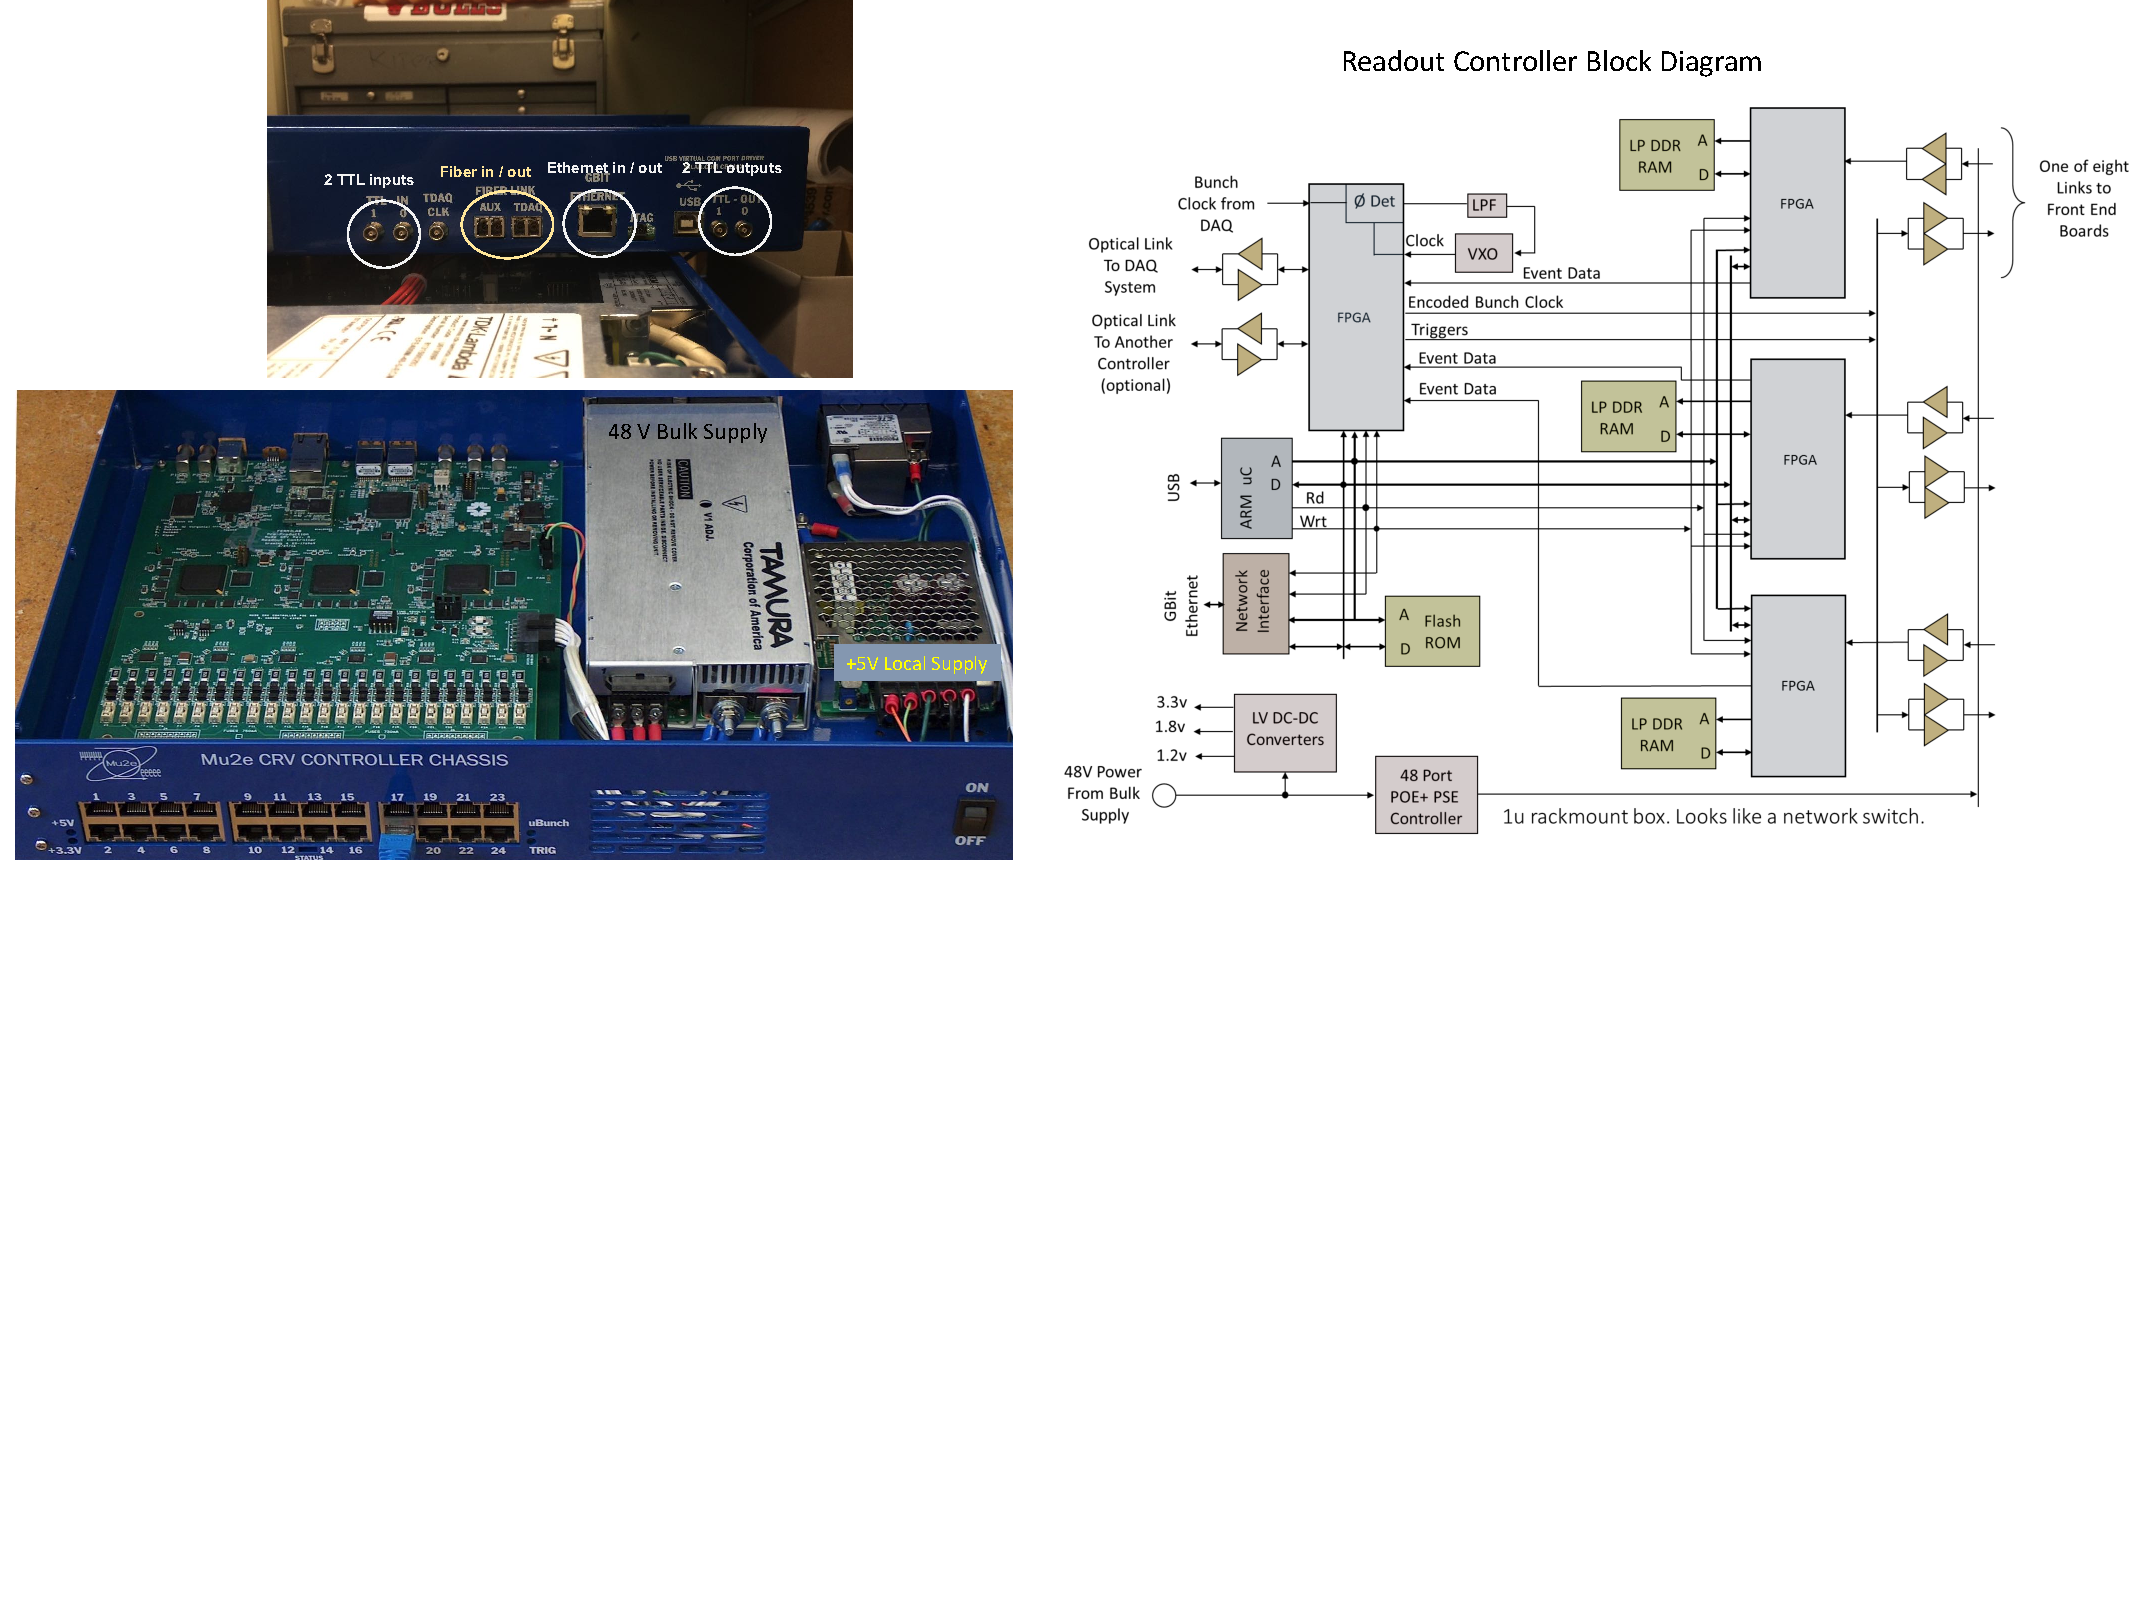
\includegraphics[height=4.8in]{graphics/pds-controller.pdf} 
\vspace{-5.5cm}
% \fixme{Need a version of this figure without the white text overlay.}
\end{dunefigure}

%\begin{figure}[h]
%\begin{centering}
%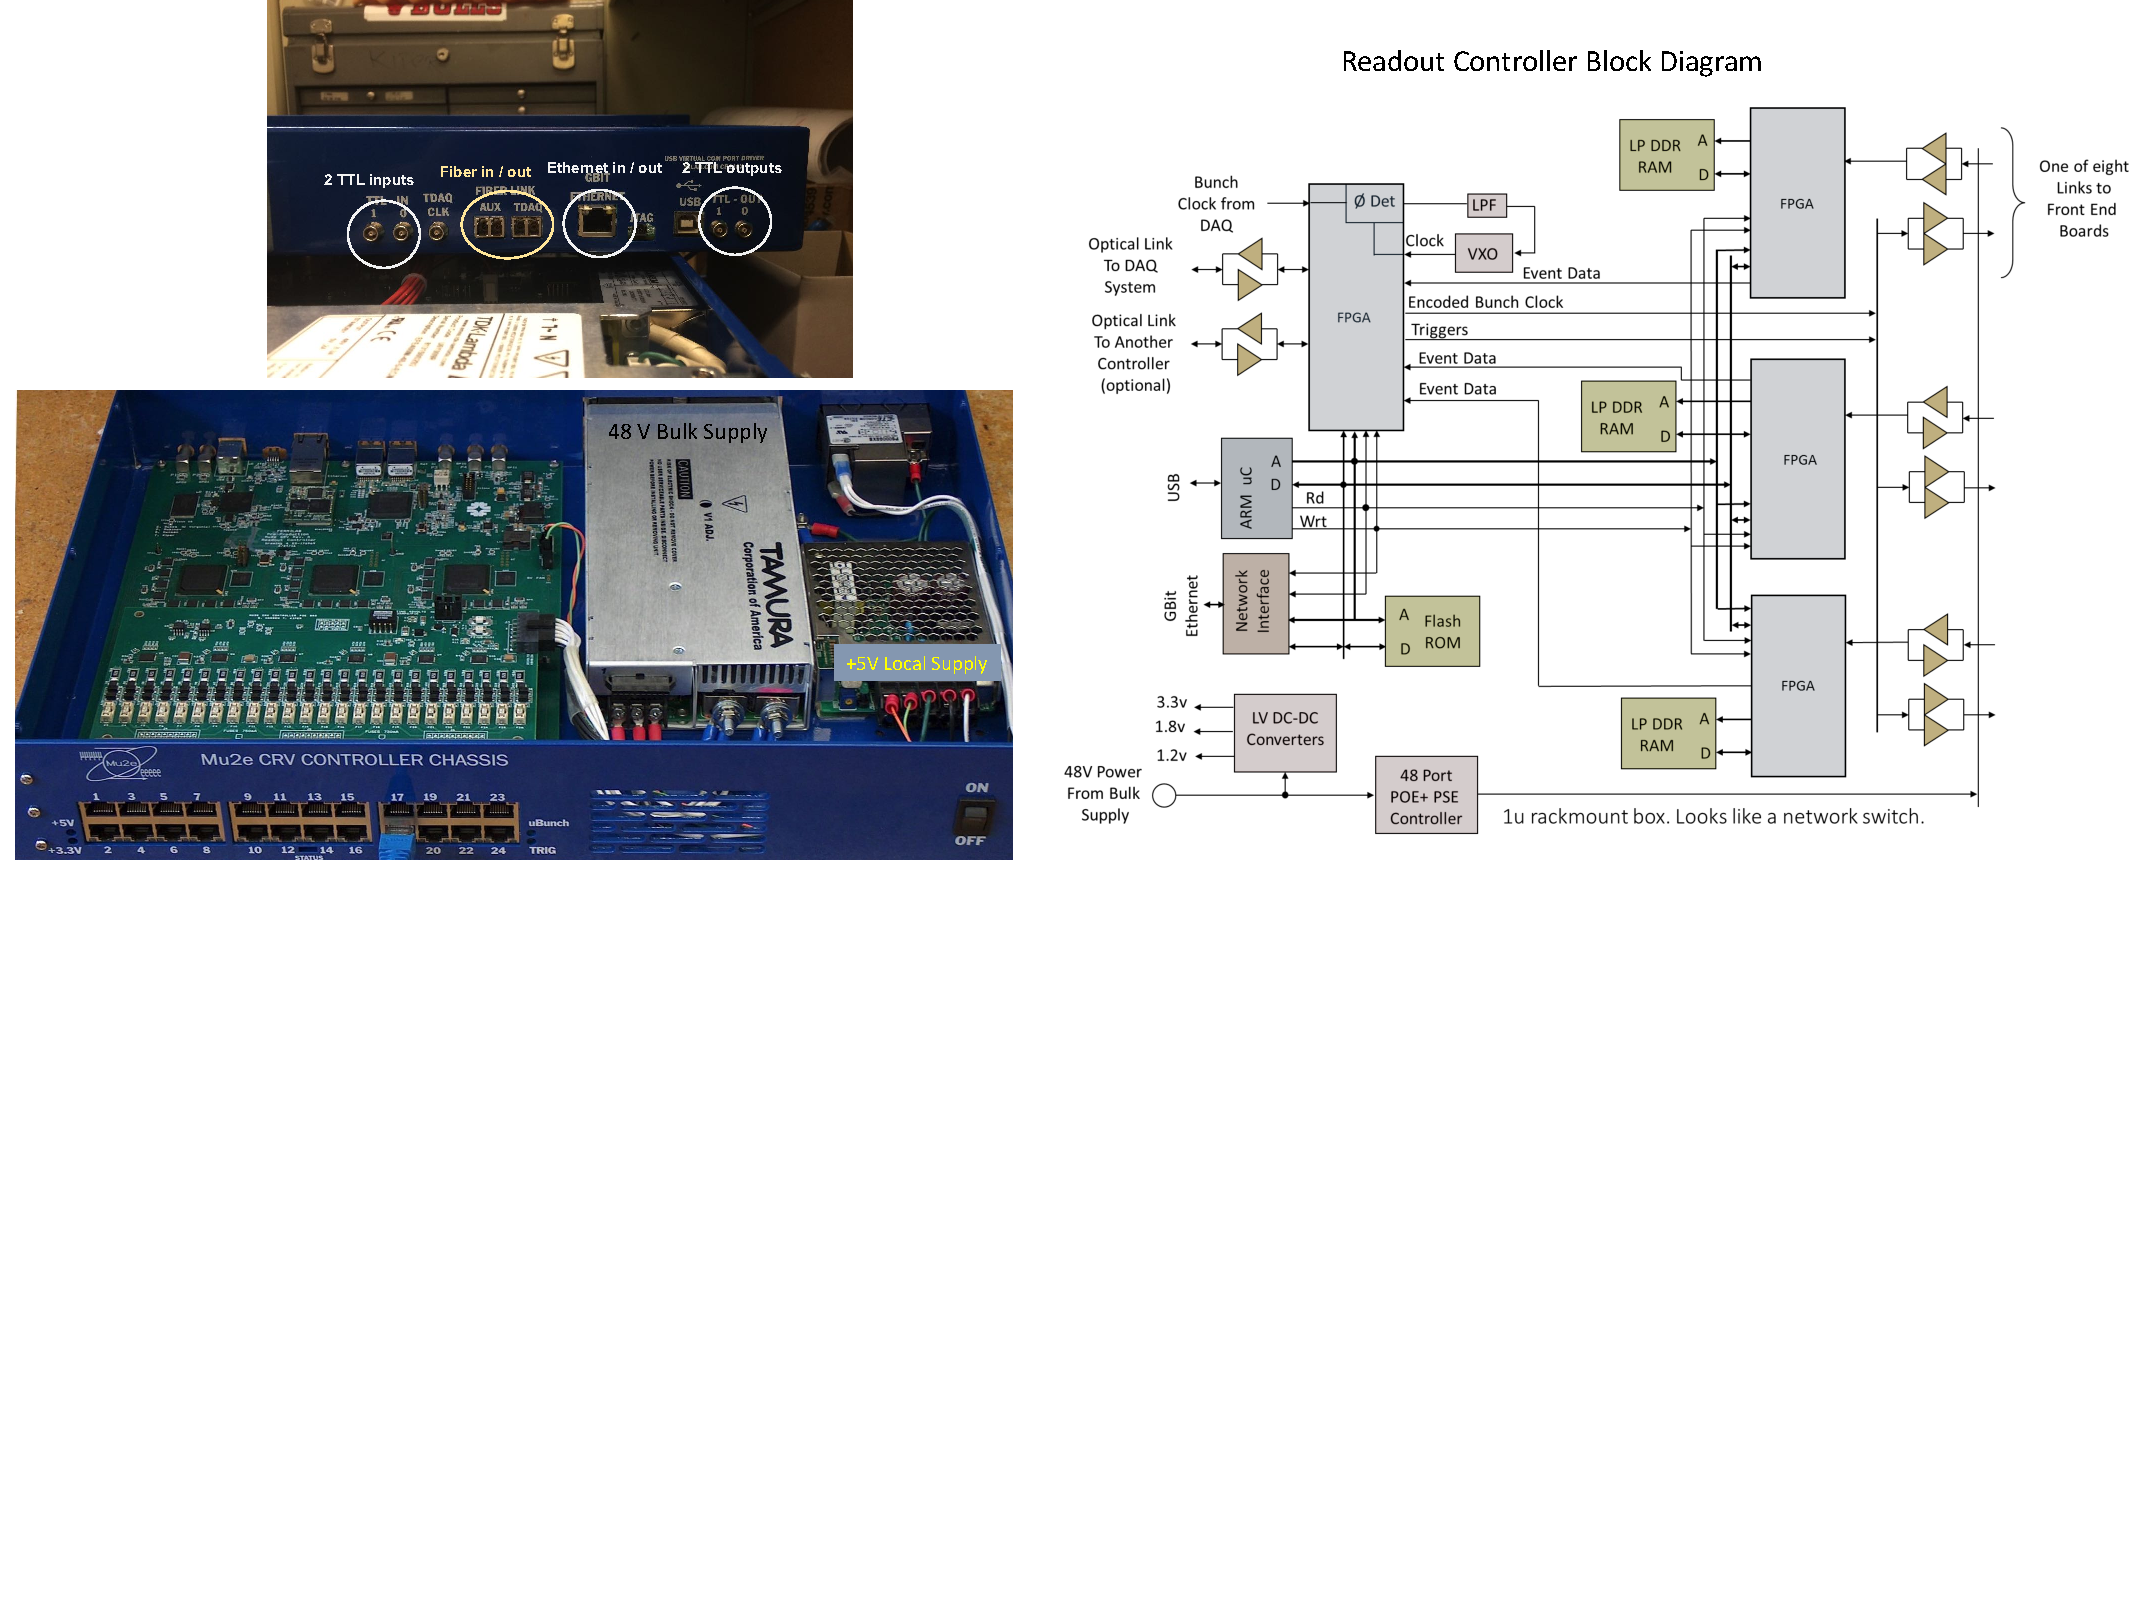
\includegraphics[height=4.8in]{graphics/pds-controller.pdf} 
%\vspace{-5.5cm}
%\caption{Left: The front and back views of the controller module, which is capable of accepting signals from 24 FEBs.  Right: A schematic of the controller.}
%\label{fig:controller}
%\end{centering}
%\end{figure}

\begin{dunefigure}[\dword{pds} front-end electronics grounding scheme.]
 {fig:grounding_power}
 {Grounding scheme with 1 chassis, containing 12 FEBs, a controller module, and a DAQ PAC, as an example (left); power and data link arrangement of the FEB and controller (right).}
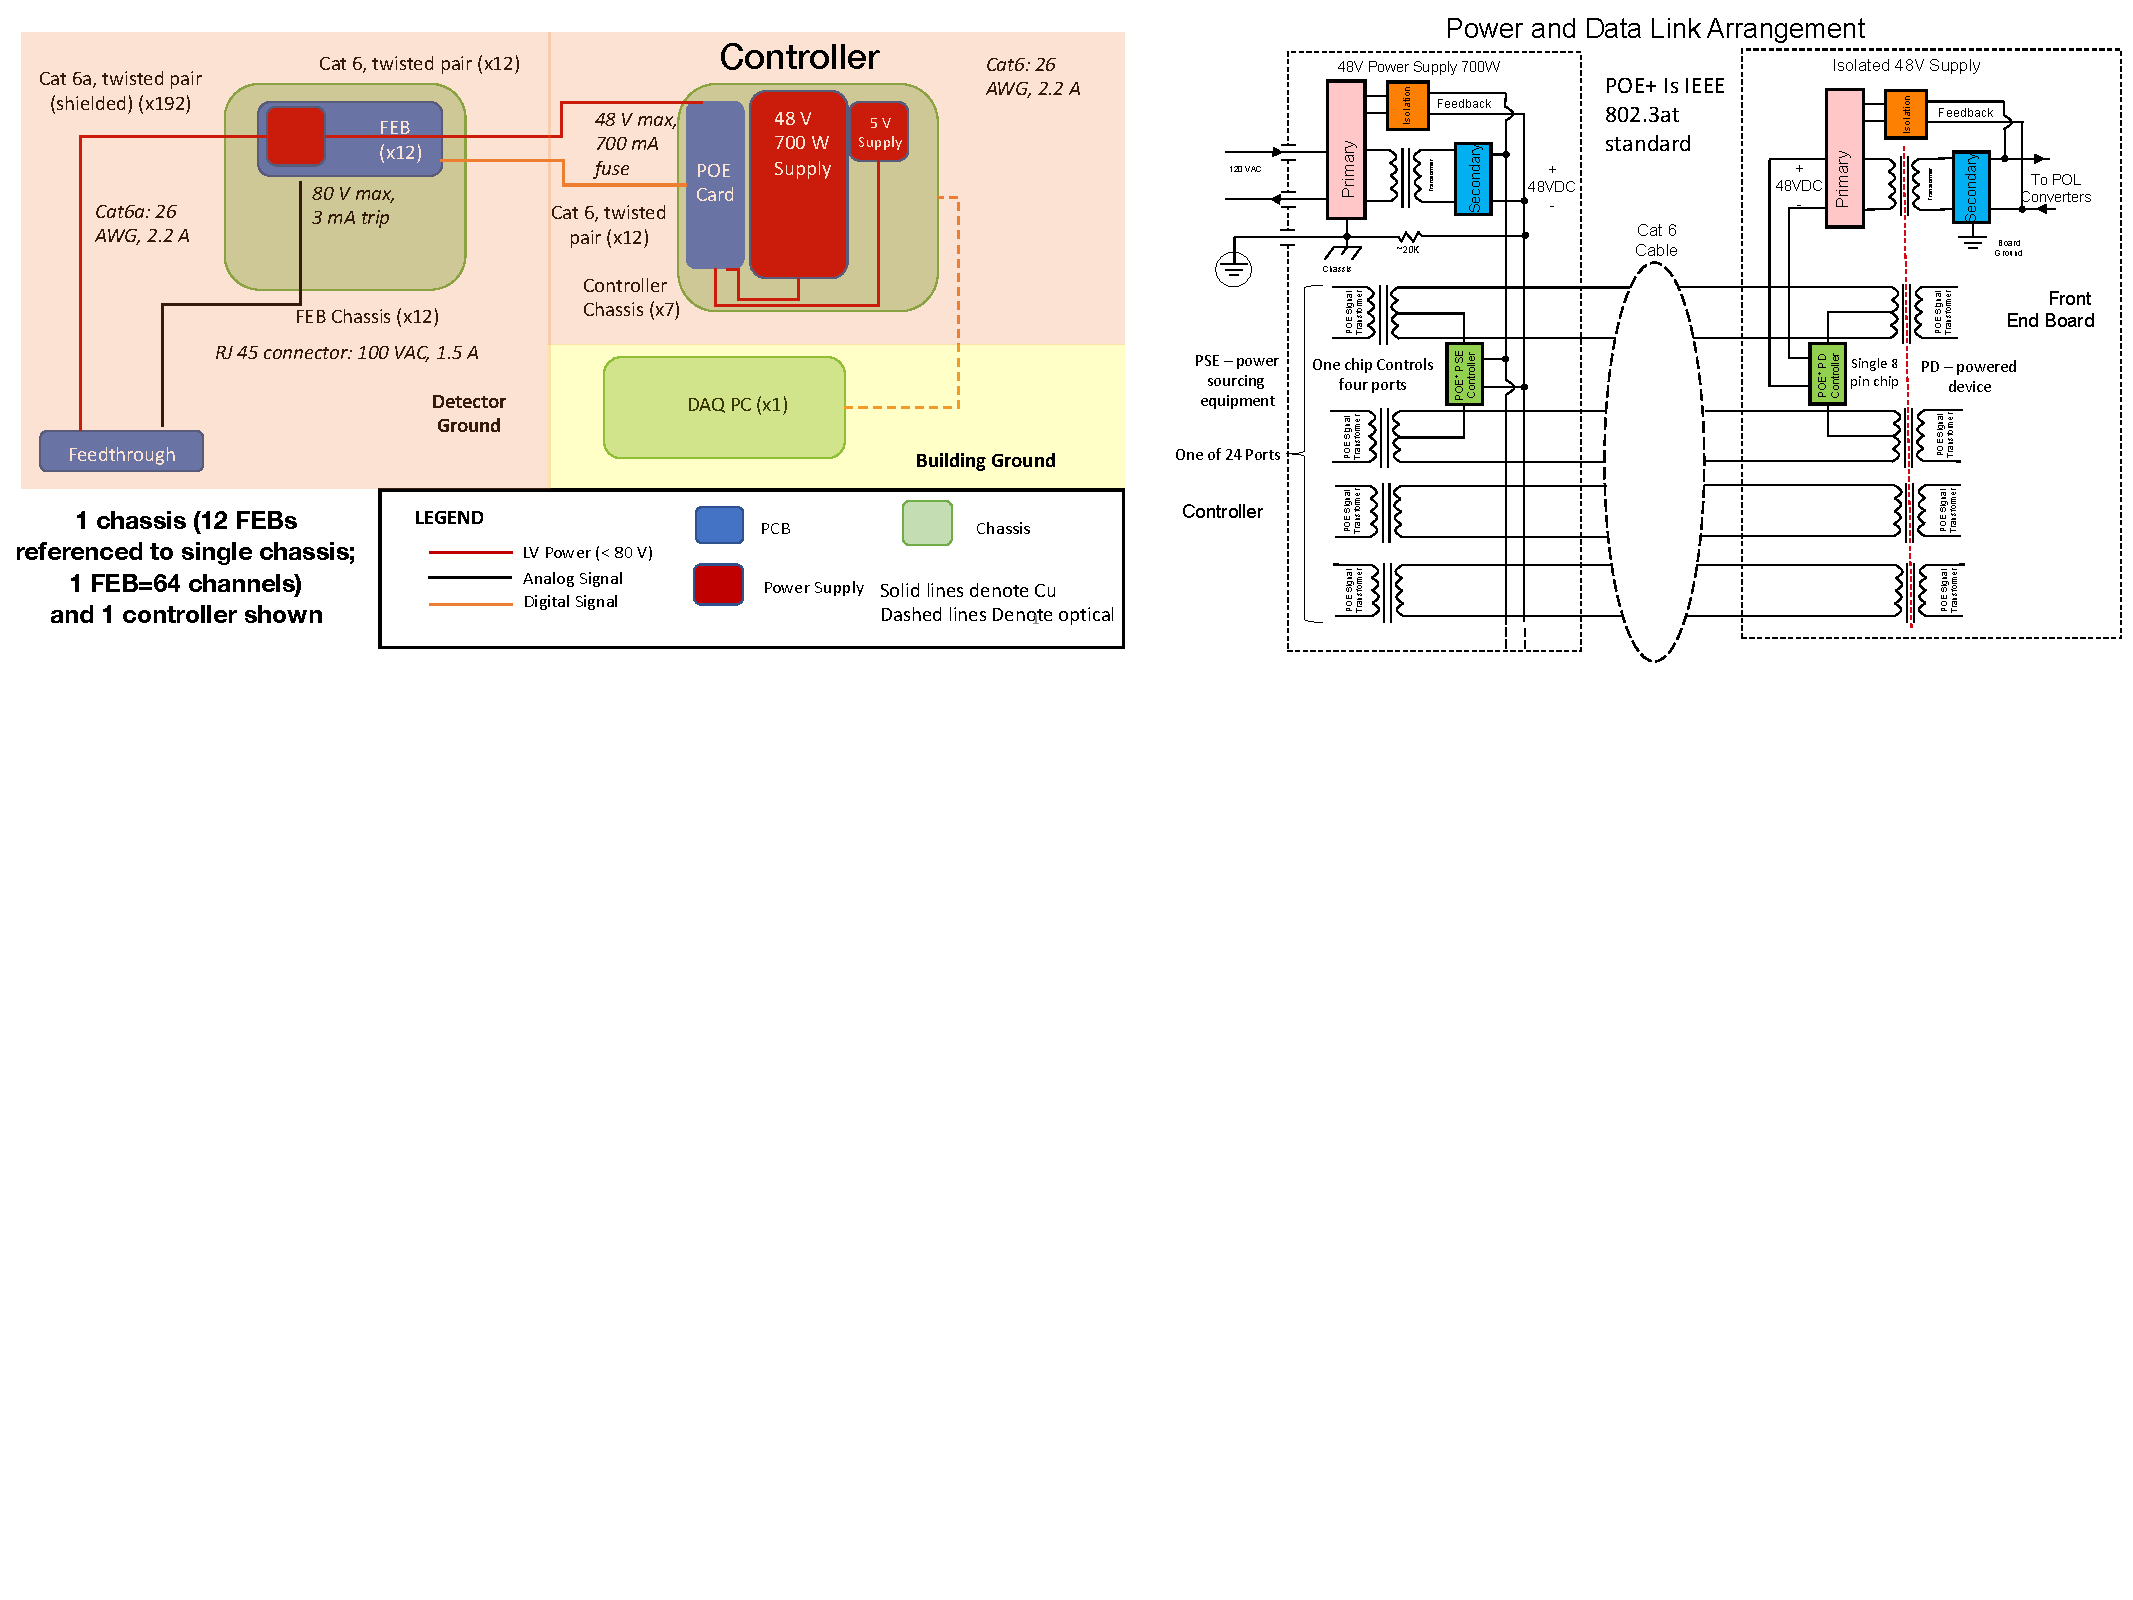
\includegraphics[height=4.8in]{graphics/pds-grounding-power.pdf} 
\vspace{-7.1cm}
\end{dunefigure}


%\begin{figure}[h]
%\begin{centering}
%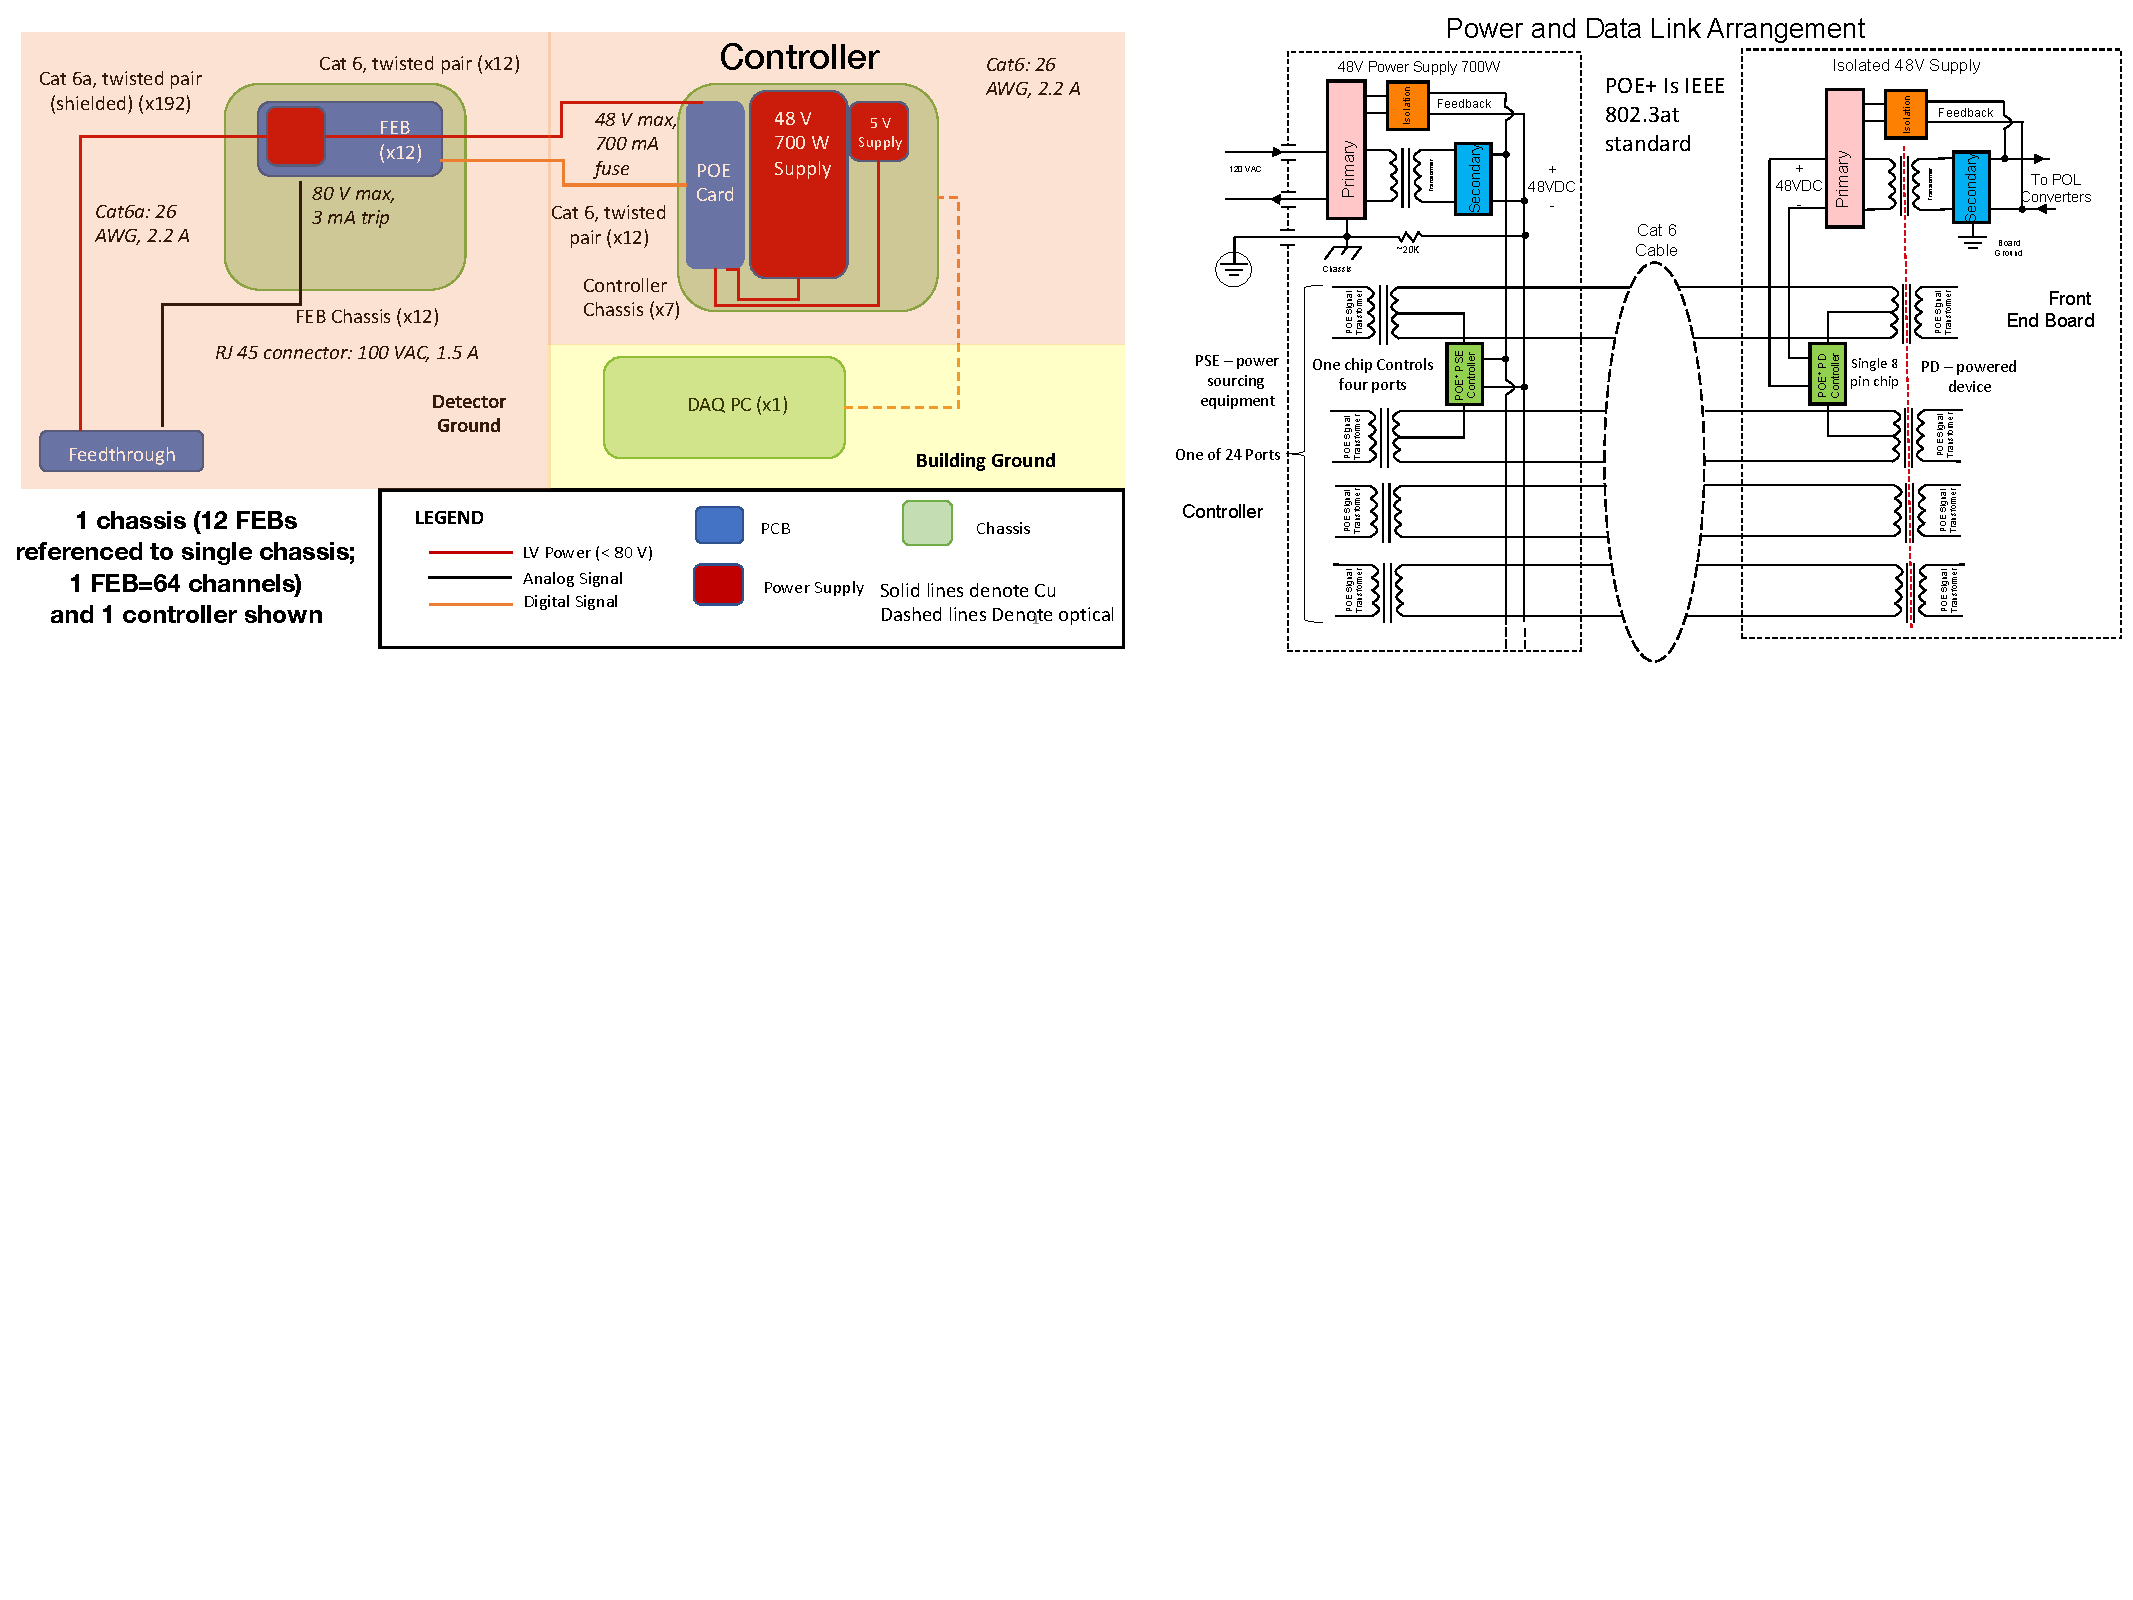
\includegraphics[height=4.8in]{graphics/pds-grounding-power.pdf} 
%\vspace{-7.1cm}
%\caption{(Left) The envisioned grounding scheme with 1 chassis, containing 12 FEBs, a controller module, and a DAQ PAC, as an example. The power and data link arrangement of the FEB and controller.}
%\label{fig:grounding_power}
%\end{centering}
%\end{figure}
%%%%%%%%%%%%%%%%%%%%%%%%%%%%%%%%%%%%%%%%%%%%%%%%%%%%%%%%%%%%%%%%%%%%%%%

\subsubsection{Electronics Next Steps}

%\fixme{Zelimir moved sections around 11/29/2018, and also made a pass through the text below.}
%\fixme{updated by Toups 11/28/2018}

%Toups start - 11/28/2018
Although the FEBs developed for the Mu2e cosmic ray veto and proposed here for use in DUNE have been demonstrated to read out an array of \dwords{mppc} with an adequate signal-to-noise ratio to provide sensitivity to single photons, there are a number of optimization and development tasks that are being pursued:  
\begin{enumerate}
\item The warm readout electronics presented here assume that only 48 out of the 64 channels on the Mu2e FEB are populated to better match the 40 ProtoDUNE channels per APA.  A prototype board will be produced to test this configuration and validate the associated cost model.  
\item The Mu2e warm readout electronics use last-generation (Xilinx Spartan-6) FPGAs and other components that have since been superceded by newer devices.  Design and prototyping work will be done to incorporate newer FPGAs (Xilinx Spartan-7 or Artix-7) into the electronics, which will improve their performance and maintainability over the lifetime of the DUNE experiment. The Artix-7 FPGAs have been implemented with \dword{ssp} readout system used in \dword{pdsp} and therefore the expertise with these system components has been established. 
\item Results from the ICEBERG test stand can determine whether there are sufficient logic resources in the FPGAs to meet a broad range of possible DAQ requirements expected from the warm readout electronics. To that end the low-cost front-end solution will be compared to existing 14-bit, 150 MS/s \dword{ssp} readout. At present, straightforward zero suppression schemes that can be implemented on the mu2e board with the current Spartan-6 FPGA will be tested with respect to potential DAQ data rate limitations.  However, increases in the number of logic cells can be accommodated by switching to more capable but still pinout-compatible devices within the same Xilinx FPGA family as discussed above.  
\item It may be desirable to increase the dynamic range of the ADCs used on the FEBs in order to achieve desired physics goals related to the energy resolution of beam neutrino events.  To this end, work should be done to investigate replacing the TI AFE5807 ultrasound chip with the TI AFE5808 ultrasound chip, which is pinout compatible but incorporates a 14-bit ADC.  Ultimately, a prototype board will need to be built incorporating all of the optimizations and improvements listed above.
\end{enumerate}
%Toups end - 11/28/2018
%Although the requirements for the electronics system are not all fully established, it not expected that the system requires novel high-risk techniques and can be developed and fabricated well within the schedule for the \dword{pds}.
In late CY18, \dword{pdsp} test beam and cosmic-ray muon data analysis will provide evaluation of the readout system implemented in \dword{pdsp} and the \dword{pd} Photon Sensor and Simulation groups will provide guidance on readout requirements discussed above. Additional data from ICEBERG and other test-stands will be collected to inform final requirements.

%As identified in Section~\ref{sec:fdsp-pd-ps}, the most important near term R\&D program will be to optimize the ganging scheme including choice of \dword{sipm} and cable types. 
%The first objective is to demonstrate that an ensemble of \numrange{48}{72} Hamamatsu \SI{6}{mm}$\times$\SI{6}{mm} \dwords{mppc} can be summed into a single channel by a combination of passive and active ganging. This board will also measure the photoelectron collection efficiency when the \dwords{sipm} are coated with \dword{tpb} as a reference for ARAPUCA measurements with a similar ganging level (the summing  board is the same size as the \dword{pdsp} ARAPUCA backplane to facilitate the comparisons).
%Charge processing requires a charge preamplifier ideally located within the cold environment, so the design must take into consideration the failure risks and the power dissipated into the environment.

%The timing resolution, minimum threshold and dynamic range requirements for the system are dictated by the physics requirements. These are well known for the higher energy physics (>\SI{200}{MeV}) but, as noted elsewhere in this document, are still evolving for lower energy. Currently,  a timing resolution of 1$\mu$s is called for and the sampling rate and number of sample bits is estimated based on this. For this task some digital process such as a sample interpolation may be proposed, enhancing the recorded raw sample time precision.
%The light sensitivity and the dynamic range requirement will determine the number of bits and the sample rate required by either waveform or charge collection methods. In both cases, the signal to noise ratio and the power consumption must be estimated.  
%With this data from \dword{pdsp} and the ganging studies, the choice between waveform readout and integrated charge readout will be made taking into account DAQ readout and trigger requirements and, in general, the physics requirements of the experiment. 
% rjw 12/3/18 Per email from Matt Toups - previous paragraph not needed
%\fixme{rjw Is this still an open question for the baseline?}


%%%%%%%%%%%%%%%%%%%%%%%%%%%%%%%%%%%%%%%%%%%%%%%%%
\subsection{Calibration and Monitoring}
\label{sec:fdsp-pd-CandM}
%\metainfo{\color{red}\bf  Content: Djurcic}

%\fixme{New section on the Calibration and Monitoring system design here - provided by dj 11/25/18 - thanks!} 
%\fixme{Note there is a section in the Production and Assembly needed too.}

%%%%%%%%%%%%%%%%%%%%%%%%%%%%%%%%%%%
% provided by dj 11/25/18
% Note: The section on protodune experience in the file is moved to the pds-validation section
%\subsection{Calibration and Monitoring}
%\label{sec:fdsp-pd-calib}

%\subsubsection{Introduction}

The photon detection system will incorporate a monitoring and calibration that will meet the physics requirements of the DUNE experiment. The pulsed UV-light system described in this section will be used to verify the photon detector gain, linearity, and timing resolution; and to monitor stability and the system response over time.  Figure~\ref{fig:pds_calmon_fig1} shows a cartoon of the placement of the system in the TPC. The system will also be an important detector commissioning tool: before closing the cryostat, 
in the cool-down phase, and when it is being filled with \lar.
%- to test the photon detectors, to generate test conditions for low-energy physics, and to 
%make use of it for quick reliable test of PDS when a change in configuration is made.
%	=> Don?t have to wait for cosmic muon coverage of entire detector
Other complementary calibration systems, such as radioactive sources, will be described in the TDR Calibration chapter (Chapter~7). 

\fixme{a figure showing the design elements?}

\begin{dunefigure}[\dword{pdsp} photon-detector calibration and monitoring system.]
 {fig:pds_calmon_fig1}
 {Schematic of the \dword{pdsp} photon-detector calibration and monitoring system.}
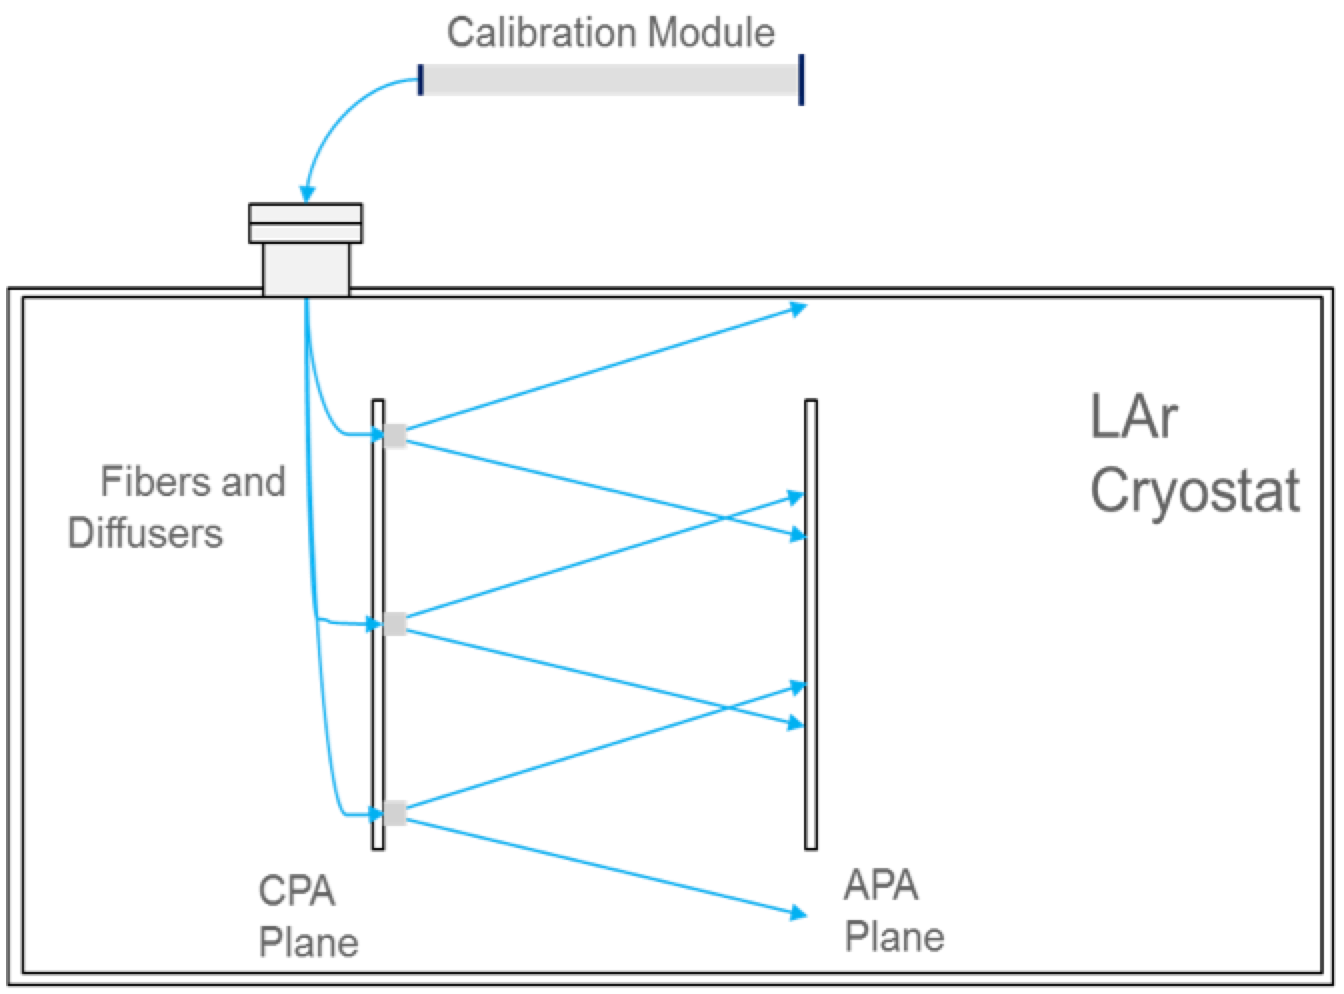
\includegraphics[angle=0,width=8.4cm,height=6cm]{graphics/pds-calmon-fig1-old.png}
\end{dunefigure}

The system hardware consists of both warm and cold components. Diffusers mounted on the cathode planes (\dwords{cpa}) provide light sources illuminating photon detectors embedded in the anode planes. These light diffusers uniformly illuminate the APA area containing the \dword{pds} light-collection modules. Cold components (diffusers and fibers) interface with High-Voltage systems design. 
Diffusers are installed at CPA, and therefore reside at the same CPA potential. 
Quartz fibers are insulators used to transport light from optical feedthroughs (at the cryostat top) through Field Cage ground plane, and through Field Cage strips to the CPA top frame. These fibers are then optically connected to diffusers located at CPA panels. 
HVS requirements place a requirement on the fiber electrical resistance to ensure the cathode is protected from shorting out due to fiber conductivity. 
Warm components include controlled pulsed-UV source (245-280 nm) and warm optics. These warm components will interface the CTF with Slow-Controls/DAQ subsystems. The optical feedthrough is a part of the cryostat interface.
%describe Cali Module. Describe what calibrations could be done

The system has no active components within PDS/APA. The active system component consists of a 1U rack mount
Light Calibration Module (LCM) sitting outside the cryostat. The LCM generates light pulses that propagate through a quartz fiber-optic cable to diffusers at the CPA to distribute the light uniformly across the photon detectors mounted within the APA.
The LCM utilizes the logic and timing control developed to meet DUNE DAQ requirements. It consists of an FPGA-based control logic unit coupled to an internal LED Pulser Module (LPM) and an additional bulk power supply. The LPM utilizes multiple digital outputs from the control board to control the LPM pulse
amplitude, pulse multiplicity, repetition rates, and pulse duration. The unit relies on dedicated Digital to Analog Converters (DACs) used to control the LPM pulse amplitude. Internal ADC channels are used to read out a reference photodiode used for pulse-by-pulse monitoring of the LED light output. 
The output of the monitoring diode is available for normalizing the response of the SiPMs in the detector to the monitoring pulse.

Hardware components will be designed and fabricated based on expertise gained with \dword{pdsp} prototype system described in Section~\ref{sec:fdsp-pd-validation-candm}.
%PDS Calibration/Monitoring system that is planned to have components installed with the HVS Cathode, and through Field Cage strips and File Cage ground plane. 
%Interface documents describe the necessary interfaces for both SP-PDS and HVS to complete the design, fabrication and installation of their subsystems.
%(need a schematics here)

\subsubsection{Next Steps}
\fixme{Much of this may belong in the System Interface section of this chapter.}

In the next steps there will be continued interface discussion with Cryostat/DSS group to identify feed-through ports/locations and to define fiber routes along DSS. The calibration TF and PDS group will share rack spaces. There won't be dedicated ports for all calibration devices e.g. laser and cameras will share ports. 
Therefore, multi-purpose ports are planned to be shared between various groups. CTF and SP-PDS will define ports for deployment. It is possible that SP-PDS might use Detector Support Structure (DSS) ports or TPC signal ports for routing fibers. CTF will be responsible for interlocks needed with other calibration devices 
like laser, radioactive sources etc. SP-PDS will not provide the interlock mechanism, but within interface between SP-PDS and CTF a system that will avoid turning  on other light sources when PDS is in operation will be defined.
It is also planned to continue work with HV/CPA groups to identify optimal materials and locations of photon diffusers at CPA, to define fiber routes and connector locations  at CPA, and to define diffuser/fiber installation procedures.

The following additional steps will be completed before fabrication and installation of the photon-detector calibration and monitoring systems proceeds: add feedthroughs to cryostat drawings, diffuser/fiber to CPA/HV drawings; diffuser material selection, prototyping, production and QA/QC testing; fiber selection, prototyping, production and QA/QC testing; identify, test and procure VUV light sources; productions and testing of calibration modules; define integration and installation of system components.



\subsection{Options to Enhance Light Yield Uniformity}
\label{sec:fdsp-pd-enh}
%\metainfo{\color{blue} Content: Cavanna/Whittington/Machado/Escobar}
%\fixme{add intro text}
 
Due to a combination of geometric effects and the impact of Rayleigh scattering, the baseline \dword{pds} design will result in non-uniformity of light collection along the drift direction. Light emitted from interactions close to the \dwords{apa} has an order of magnitude larger chance of being detected compared to interactions close to the \dword{cpa}. 

Though the designs described in the previous sections will meet the \dword{pd} performance requirements we have considered two options for enhancing both the light yield and light yield uniformity.  Both approaches mitigate the impact of a short Rayleigh scattering length by converting \SI{127}{nm} scintillation photons to longer wavelength photons with a significantly longer Rayleigh scattering length. A benefit of the increase in uniformity is that it will enhance the ability to do calorimetric reconstruction with scintillation light; this would enhance the charge-based energy reconstruction as well as increase the efficiency of triggering on low energy signals.

These options will be pursued in parallel with the baseline design and may be implemented after appropriate review if resources are available and if they do not interfere with or produce unacceptable risk for the baseline design schedule.


%>> Start: Andrzej Szelc 14/02/2018 >>>>>>>>>>>>> 
% Not a publication, but a proceedings:  To cite this article: Diego Garcia-Gamez and SBND Collaboration 2017 J. Phys.: Conf. Ser. 888 012094

\subsubsection{Coated Reflector Foils on the TPC Cathode}
\label{sec:fdsp-pd-enh-cathode}

In this option, scintillation light falling on the cathode plane is converted into the visible wavelengths. This light, instead of being absorbed on the \dword{cpa}, could then be detected by the photon detectors embedded in the \dword{apa} improving the overall collection efficiency. In this scheme the light collector must be sensitive to visible light. 

This can be achieved in two ways: by coating the X-ARAPUCA with TPB instead of pTp, which results in the same WLS combination as the double shift bars (whose performance is measured in \dword{pdsp})
and/or by leaving some of the X-ARAPUCA detectors uncoated with a WLS and an apropriate dichroic filter. In the former case the detectors are sensitive to both the direct and reflected light, in the latter case only to the reflected light. 

Fig.~\ref{fig:ly_with_foils}, shows the simulated results of a configuration where 50\% of the \dword{apa} light collectors are capable of recording both direct scintillation light and the visible light from the \dword{cpa} and 50\% are left uncoated to maximize uniformity. This results in an enhancement of the total light collection close to the cathode (black points), which will increase the detection efficiency in that region. 

Introducing the foils on the cathode may also enable drift position resolution using only scintillation light. This requires the photon detectors to be able to differentiate direct \dword{vuv} light from re-emitted visible light (e.g. two different \dword{pd} detector types) and good enough timing of arrival of first light.

Coated reflector foils are manufactured through low-temperature evaporation of \dword{tpb} on dielectric reflectors e.g. 3M DM2000 or Vikuiti\texttrademark\  ESR. Foils prepared in this manner have been successfully used in dark matter detectors such as WArP\cite{Acciarri:2008kv}. Recently they have been shown to work in \dwords{lartpc} at neutrino energies, namely  in the LArIAT test-beam detector \cite{Garcia-Gamez:2017cmu}. In LArIAT they have been installed on the field-cage walls and, during the last run, on the cathode. An alternative solution would be to use Polyethylene Naphthalate (PEN) instead of TPB. This wavelength-shifter has a similar emission spectrum to TPB \cite{Kuzniak:2018dcf}, but is provided in sheets, which could greatly simplify the production and installation. The choice of using PEN depends on demonstrating that its performance holds in liquid argon - these studies are ongoing. 

\fixme{Need the Kuzniak reference added to the bibliography.}

%The necessity to record both \dword{vuv} and visible photons in the light collectors would require a change in the current design but is conceptually possible. For example, if the cathode plane were coated with tTP,  some of the ARAPUCA modules could be constructed without the pTP coating on the outer surface of the filter and benefit from the same photon trapping effect but these cells would no longer be sensitive to direct scintillator light.   
%Understanding the impact of these competing effects on the physics is under study by the simulation group and
The method of foil installation is being developed in collaboration with the DUNE HV consortium, with the objective of minimizing the impact on the CPA design. 
In particular, the feasibility of coating the cathode with a dielectric medium is being investigated - the current solution is to prepare the foil plates with small perforations which would allow the electric field
lines to safely neutralize on the \dword{cpa} underneath. A dedicated R\&D test is being performed at CERN using the ICARUS 50l with a TPB evaporated foil on the \dword{cpa}. 

\fixme{results of this test should be ready for tdr; rjw what is the schedule for this?}


\begin{dunefigure}[Predicted light yield with WLS-coated reflector foils on the \dword{cpa}.]{fig:ly_with_foils}
{Predicted light yield in with WLS-coated reflector foils on the \dword{cpa}. Blue points represent direct \dword{vuv} light impinging on the \dwords{pd} assuming a 2.5\% photon detection efficiency and 70\% wire mesh transmission and half of the detectors left uncoated; red stars - represent scintillation light that has been wavelength-shifted and reflected on the \dword{cpa} assuming the same photon detection efficiency folded in with an 80\% transmittance of the filters to visible light. Black points show the sum of these two contributions.}
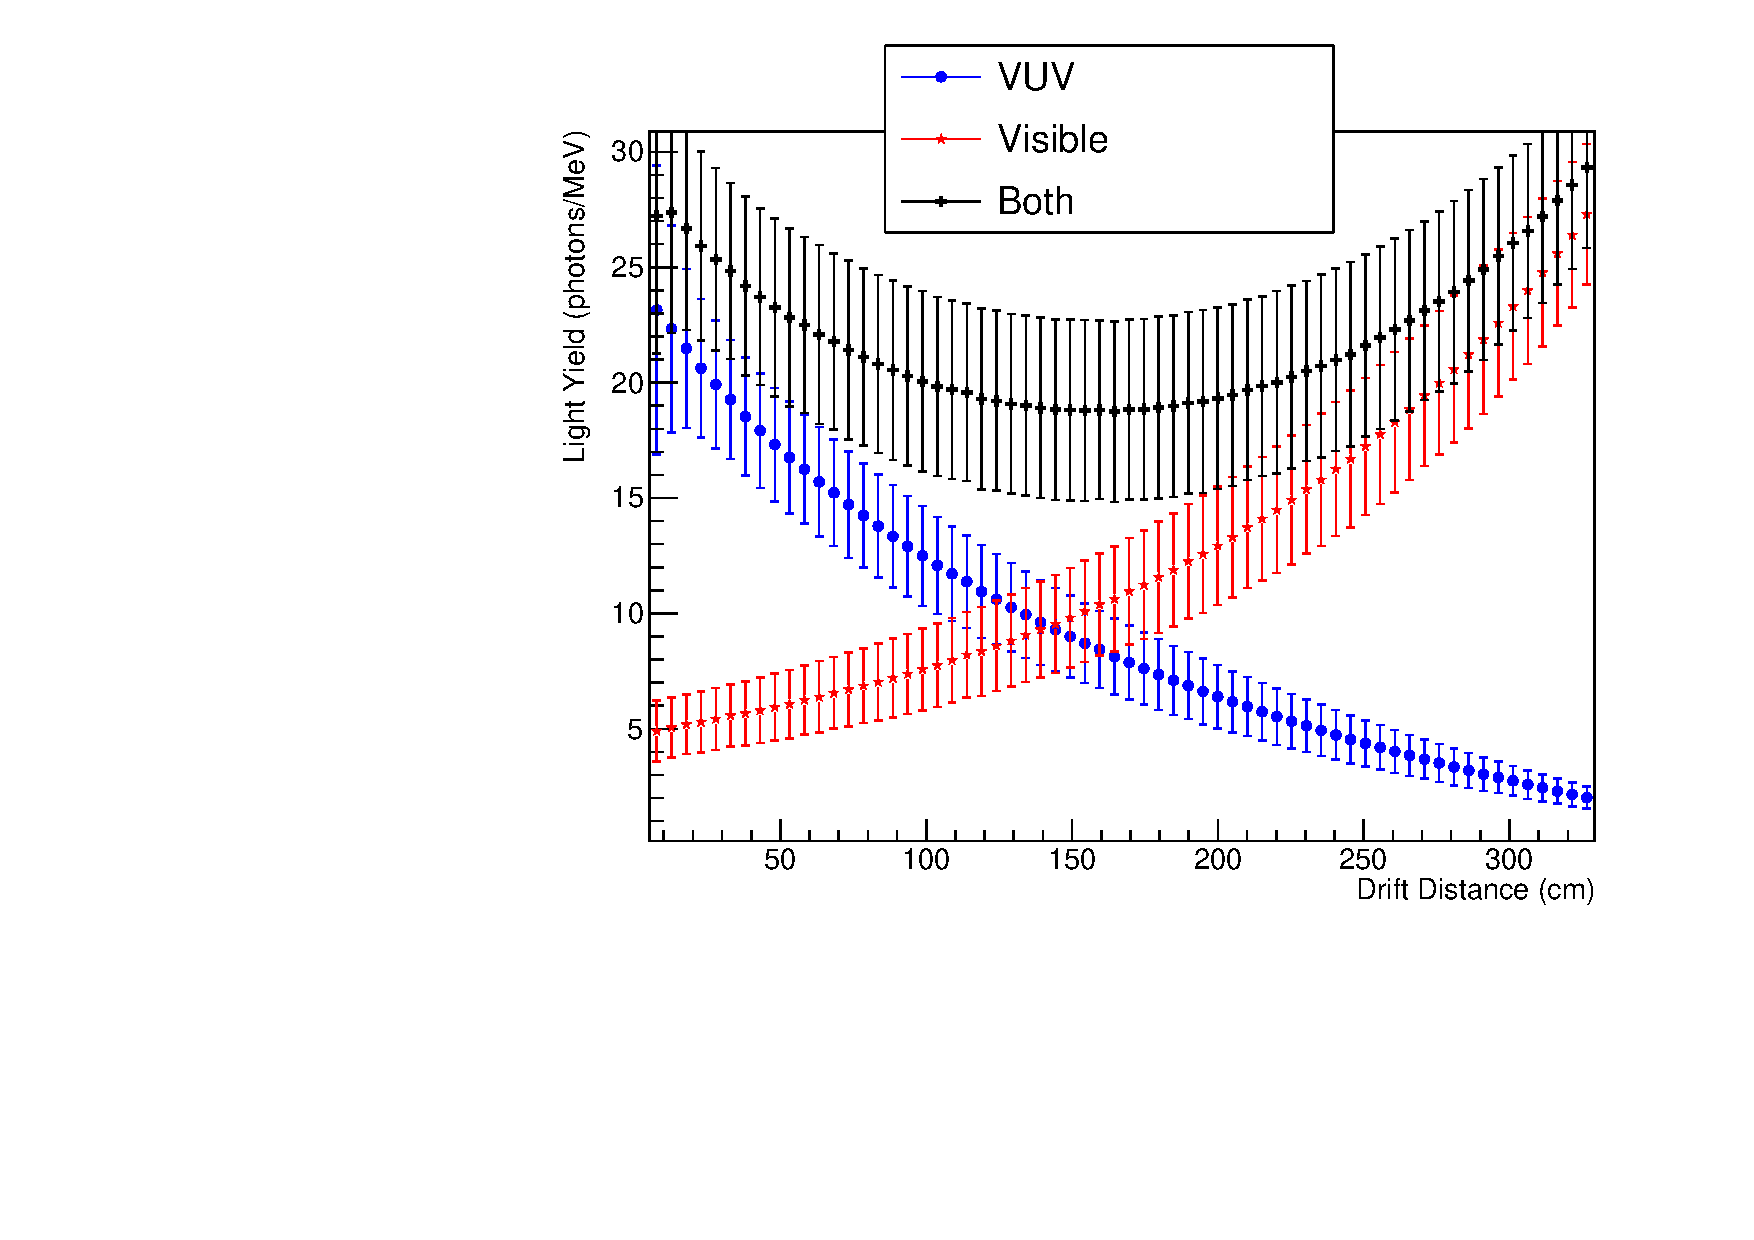
\includegraphics[width=0.4\columnwidth]{pds-ly_with_foils_new.pdf}
\end{dunefigure}

\subsubsection{Doping Liquid Argon with Trace Parts of Xenon}
\label{sec:fdsp-pd-enh-xenon}
%text edited by rjw \fixme{For now, this section is the entirety of the Word doc prepared by the xenon task force - coordinated by Carlos Escobar. Minor edits by rjw - expect will need editing down...}

%{\it\bf DUNE  Motivation and Benefits}

%The main motivation for this proposed option is to overcome the serious reduction in the response of the photon detection (PD) system to events  as they occur further from the light collectors (PC), towards the TPC cathode (CPA). Improving the response across the TPC volume will both increase the trigger efficiency and simplify the analysis for supernova neutrinos. An increased response would also be beneficial for the determination of t0 for nucleon decay events. 

This option exploits the conversion of the LAr \SI{127}{nm} light to \SI{174}{nm} by doping the LAr volume with 20-100 ppm of xenon.  While there are indications that the absolute light yield in xenon-doped argon may be higher than in pure argon, in the current estimates we assume the yields are the same. The source of the improved performance described here is the much longer Rayleigh scattering length as the light is shifted from \SI{127}{nm} to \SI{175}{nm}.  The improvement is illustrated in Fig.~\ref{fig:visibility_with_xenon} from a DUNE PD simulation, assuming an absorption length for the scintillation light of \SI{20}{m}. The gain in average yield for events near the CPA is about a factor 5.

\begin{dunefigure}[Simulation of visibility of \SI{127}{nm} and \SI{174}{nm} light.]
{fig:visibility_with_xenon}
{Simulation of visibility of \SI{127}{nm} and \SI{174}{nm} light in a \dword{sp} module.}
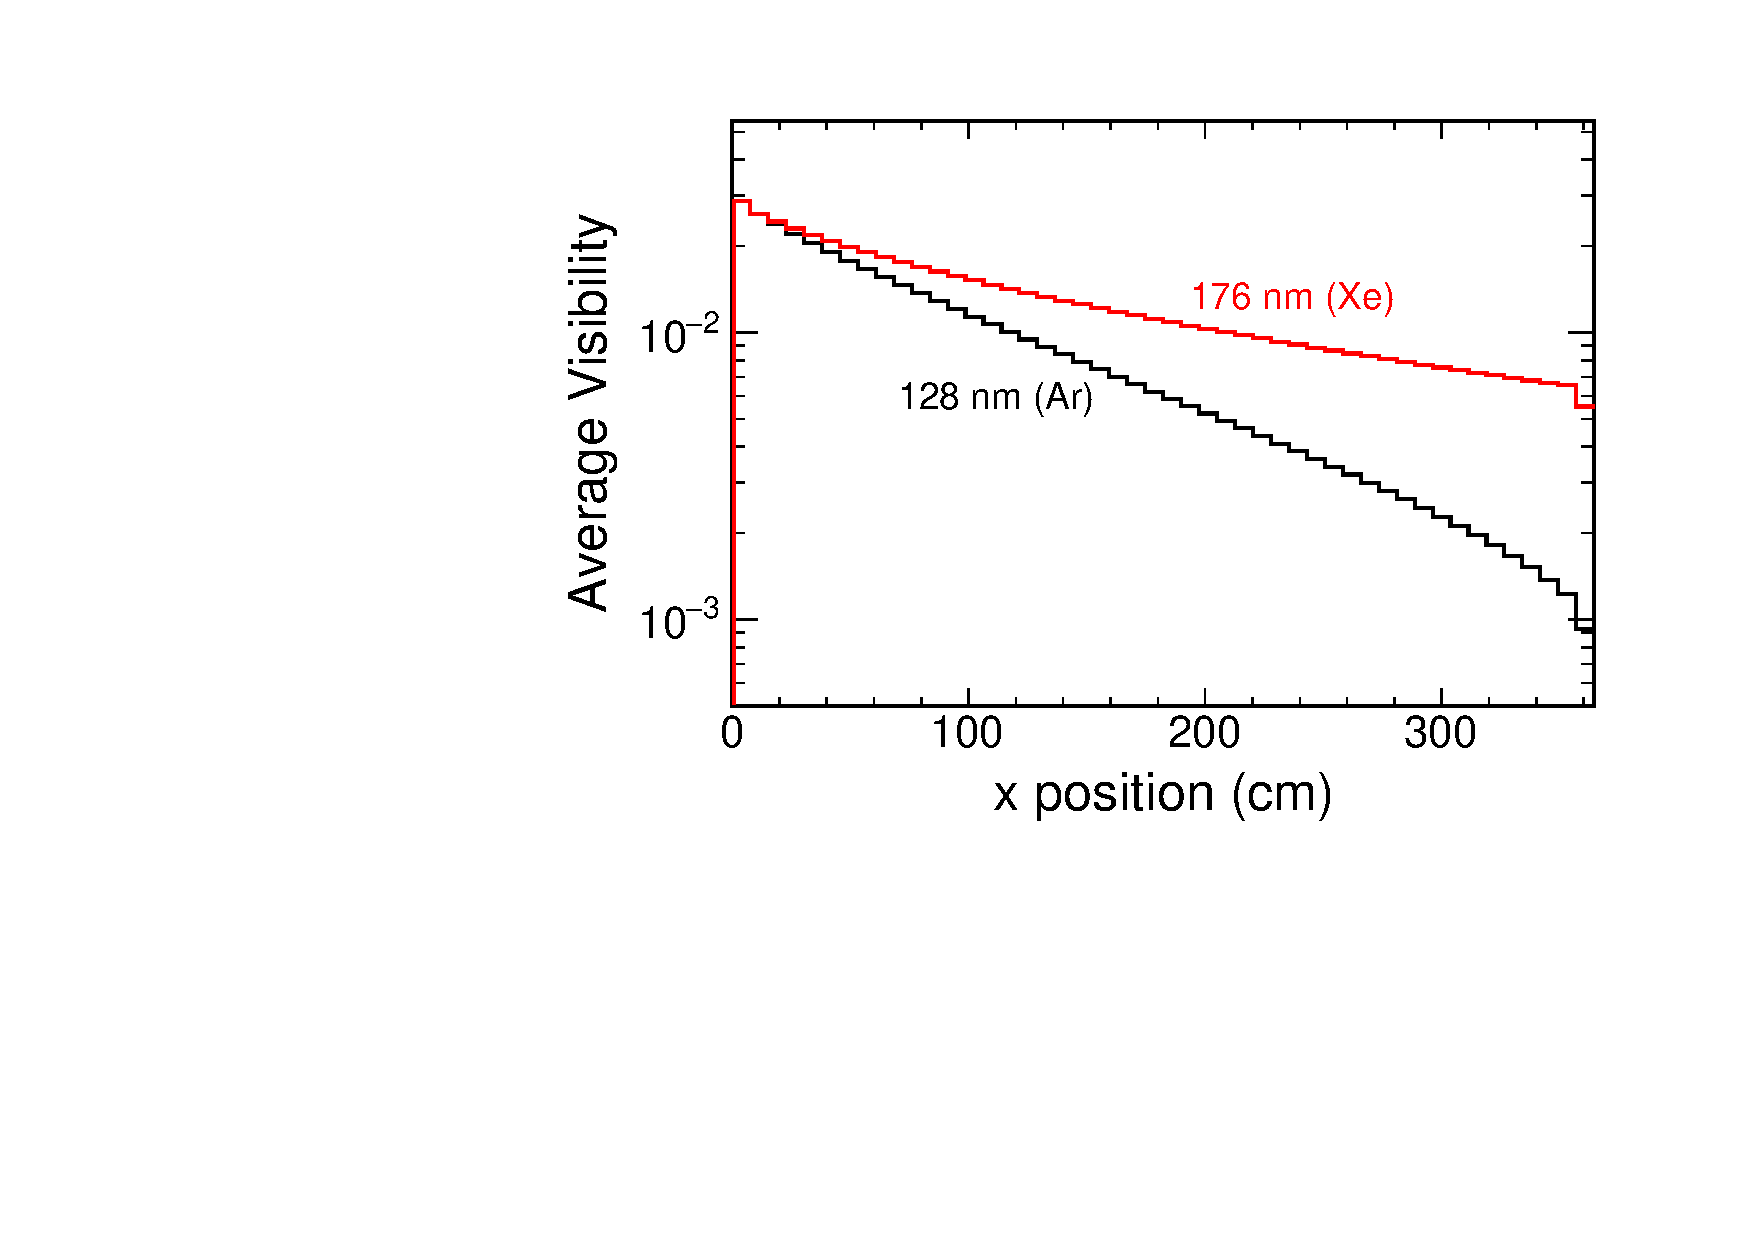
\includegraphics[width=0.5\columnwidth]{pds-ly_with_xenon.pdf}
\end{dunefigure}

Doping with xenon also affects the time structure of the scintillation light and in particular reduces the fraction of late light.  Having a light signal of shorter duration can bring advantages both in physics, such as making it easier to tag Michel electrons from pions and electrons, and in the electronics required. The longer wavelength of the scintillation light resulting from the Xe doping allows the possibility of simplifying the design of the \dword{pds} light collectors (X-ARAPUCA) by dispensing with the use of the outer layer of wavelength shifting material, thereby reducing costs and simplifying the handling of the light collectors during storage and installation. 

%{\it \bf  Implementation and rough cost}

%The diagram in Fig.~\ref{fig:cryo_with_xenon} is a schematic of the argon delivery and recirculation system for DUNE.  
Doping the argon with xenon is facilitated by the fact that at the DUNE Far Detector the argon is transported from the surface to underground as gas before it is recondensed for delivery to the cryostats. Xenon and argon can therefore be mixed in gas form before condensation;  in consultation with the cryogenic experts, we have identified locations where this mix could be achieved. Since the operations take place at room temperature, the implementation is relatively straightforward.
%the diagram shows locations where this mix could be achieved. Since the operations take place at room temperature, the implementation is relatively straightforward.

%\begin{dunefigure}[Schematic of the argon delivery and recirculation system for DUNE indicating possible locations for argon and xenon premixing.]{fig:cryo_with_xenon}
%{Schematic of the argon delivery and recirculation system for DUNE indicating possible locations for argon and xenon premixing.}
%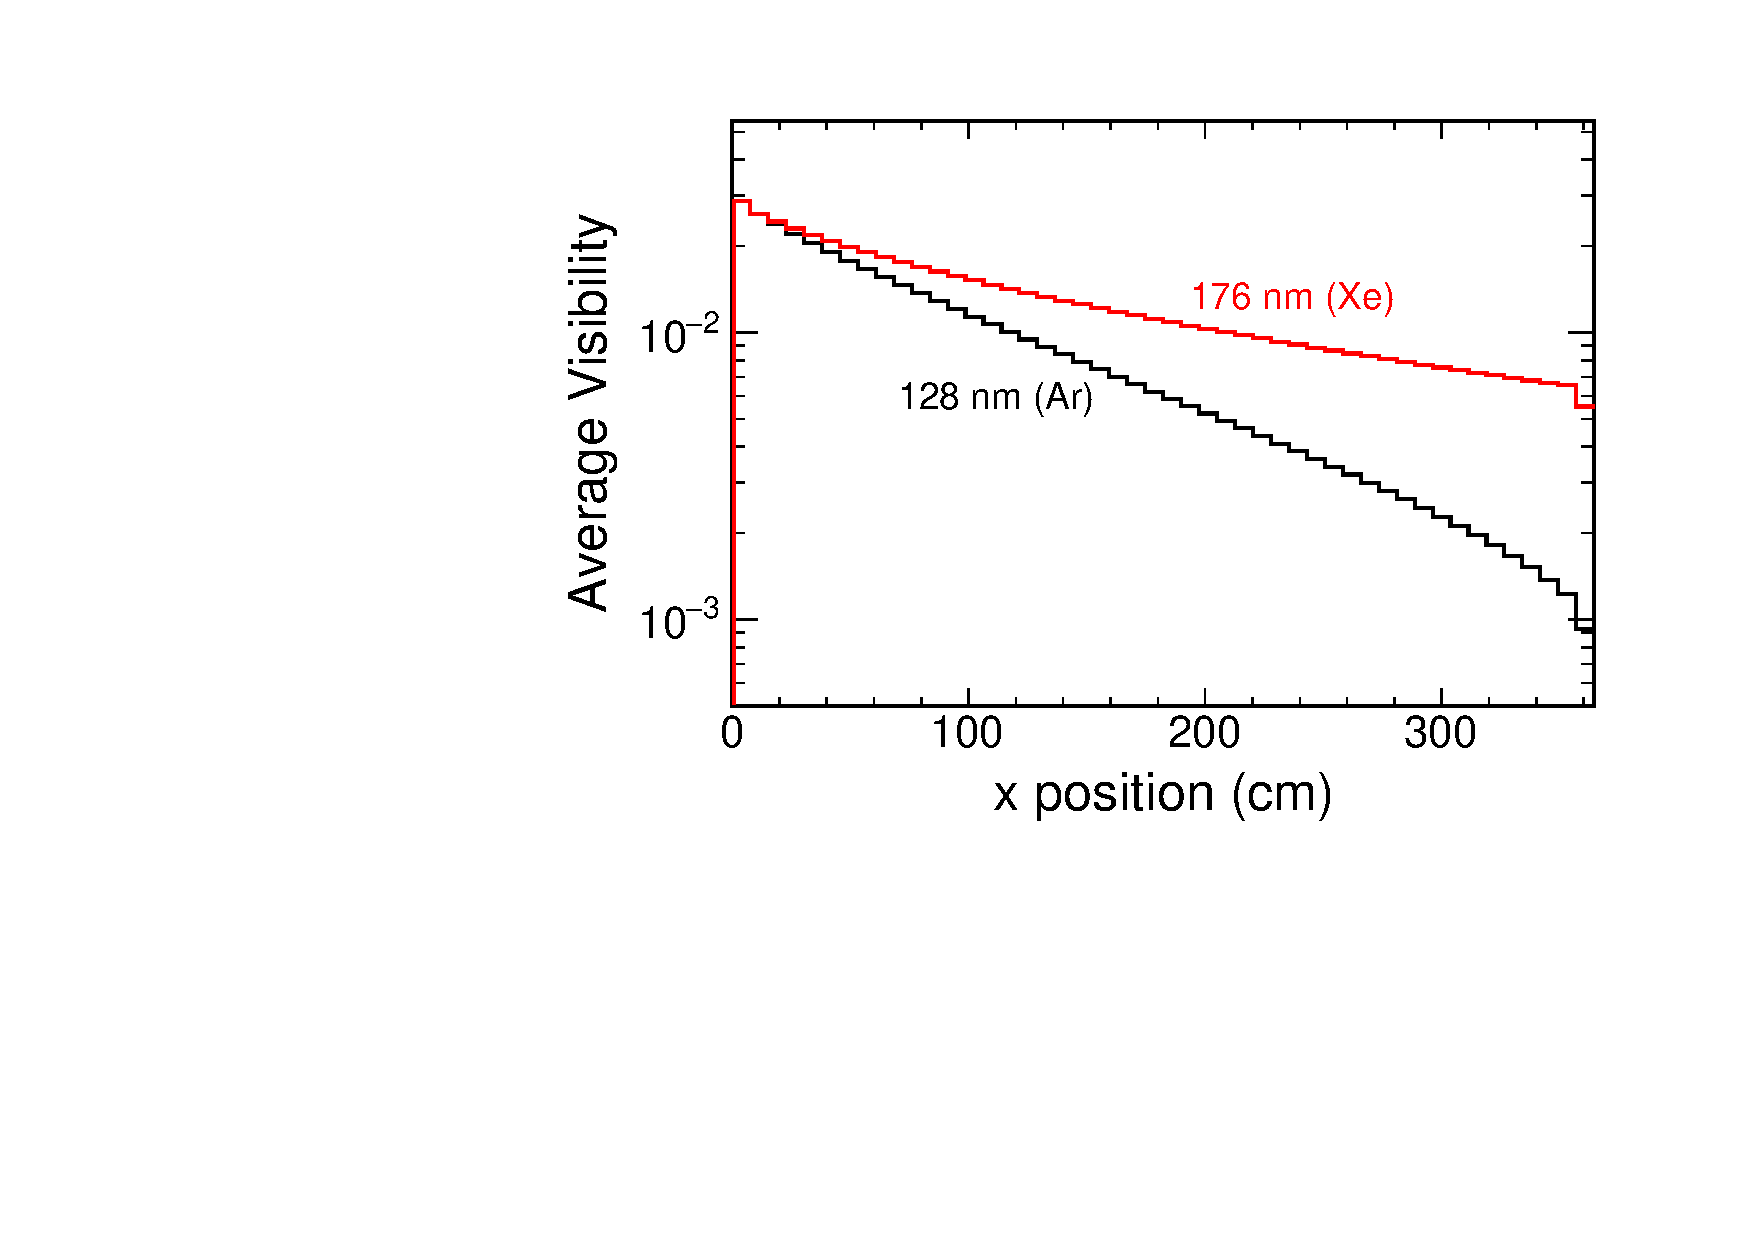
\includegraphics[width=0.6\columnwidth]{pds-ly_with_xenon.pdf}
%\end{dunefigure}

%A detailed cost estimate will require an evaluation of flow rates, piping design, etc. The major cost is expected to be the xenon, which would be ~ \$20,000/(ppm Xe doping) per Far Detector module. The physics results outlined above can be achieved for doping levels between 20 to 100 ppm of xenon.

{\it\bf Critical Issues and R\&D Work}

It is recognized that the xenon doping must not adversely affect the performance of the TPC and while the doping is expected to be neutral or even beneficial, its effects on charge yield, drift lifetime and HV stability need to be established.  There is experience in xenon doping of argon both at CERN and Fermilab, and tests for the TPC effects are being designed.  
More detailed R\&D is needed to optimize the xenon doping fraction and its interaction with the light-detection system. This can be conducted on a time scale of about a year by a small number of dedicated investigators using resources that, mostly, are expected to be available at Fermilab and CERN. 

%%%%%%%%%%%%%%%%%%%%%%%%%%%%%%%%%%%%%%%%%%%%%%%%%%%%%%%%%%%%%%%%%%%%%%%%%%%%%%%%%%%%%%%%%%%%%
\subsection{PDS Summary Table} 
\label{sec:pds-config-summary}
Table~\ref{tab:pds-config-summary} provides a summary of the \dword{pds} configuration.
\fixme{Check the table and suggest better content...}
\begin{dunetable}
[\dword{pds} Baseline Configuration Summary.]
{p{0.2\textwidth}p{0.35\textwidth}p{0.35\textwidth}}
{tab:pds-config-summary}
{\dword{pds} Baseline Configuration Summary.}
Component  				& Description 						& Quantity		\\ \toprowrule
Light Collector 		& X-ARAPUCA							& 10 modules per \dword{apa}; 1500 total (1000 single-sided; 500 double-sided)\\ \colhline
Photosensor 			& Hamamatsu \dword{mppc} \SI{6}{mm}$\times$\SI{6}{mm}	& 192 SiPM per module; 228,000 total	\\ \colhline
SiPM Signal Summing		& 6 passive x 8 active				& 4 circuits per module; 6000 total	\\ \colhline
Readout Electronics		& Based on commercial ultrasound chip& 4 channels/module; 6000 total	\\ \colhline
Calibration/Monitoring	& Pulsed UV via cathode-mounted diffusers & X per CPA; YY total			\\
\end{dunetable}

%%%%%%%%%%%%%%%%%%%%%%%%%%%%%%%%%%%%%%%%%%%%%%%%%%%%%%%%%%%%%%%%%%%%%%%%%%%%%%%%%%%%%%%%%%%%%

